\documentclass[12pt,liststotoc]{report}
\usepackage[T1]{fontenc}
\usepackage[utf8x]{inputenc}
\usepackage{color}
\usepackage{xcolor}
\usepackage{geometry}
\geometry{a4paper, top=25mm, left=25mm, right=25mm, bottom=25mm, headsep=10mm, footskip=12mm} 
\usepackage{amsfonts}
\usepackage{amsmath}
\usepackage[ngerman]{babel}
\usepackage{graphicx}
%\usepackage{subcaption}
\usepackage{booktabs}
\usepackage{tabularx}
\usepackage{array}
\usepackage{textcomp}
\usepackage{amssymb}
\usepackage{amstext}
\usepackage{subfigure}
\usepackage{amsfonts}
\usepackage{mathrsfs}
\usepackage{csquotes}
\usepackage{nicefrac}
\usepackage{multirow}
\usepackage{color}
\usepackage{bigstrut}
\usepackage[version=4]{mhchem}
\usepackage{textcomp} 
\usepackage{nicefrac}
\usepackage{lmodern}
\usepackage{pdflscape}
\usepackage{pdfpages}
\usepackage{here} 
\usepackage{pdfpages}
\newcommand{\rtab}{\raggedleft\arraybackslash}

\usepackage{hyperref}
\usepackage{fancyref}
\usepackage{todonotes}
\usepackage{bigints}
\usepackage{amsmath}
\usepackage{amssymb}
\usepackage{amstext}
\usepackage{amsfonts}
\usepackage{mathrsfs}
\usepackage[version-1-compatibility]{siunitx}
\usepackage{caption}
\captionsetup{format=plain,justification=centerlast}

%\usepackage[backend=biber,style=alphabetic,sorting=ynt]{biblatex}
%\addbibresource{Quelle_CRT_2.bib} 
 



\usepackage{ngerman}
\setlength{\parindent}{0em}	
\setlength{\parskip}{1.5ex plus0.5ex minus0.5ex}

\usepackage{chemformula}

\captionsetup[table]{skip=5pt}

%\usepackage{tikz}
%\usetikzlibrary{tikzmark}

%\newcommand\zeilestreichen[3][]{%
 % \tikz[remember picture,overlay]\draw[thick,#1]([yshift=0.8ex]pic cs:#2)--([yshift=0.8ex]pic cs:#3);}

\usepackage{soul}

\begin{document}
\setcounter{secnumdepth}{5}
\setcounter{tocdepth}{5}

\begin{titlepage}
	\centering
	
\includegraphics[width=0.5\textwidth]{Graphics/TU_Graz.pdf}\par\vspace{1cm}
	
	{\scshape\LARGE Stoffübertragung LU | Theresa Hörmann  \par}
	\vspace{1cm}
	{\scshape\Large LU 669.104\par}
	{\scshape \large SS 2018\par}
	\vspace{0.5cm}
	{\huge\bfseries $k_la$-Wert Bestimmung \par}
	\vspace{0.5cm}

	{\LARGE \itshape Ashok Andermann\par}
	{\large 11729115\par}\vspace{0.5cm}
	%\vspace{0,2cm}	
	
	{\LARGE \itshape Kilian Fleisch\par}
	{\large 11744809\par}\vspace{0.5cm}
	%\vspace{0,2cm}
	
		
	{\LARGE \itshape David Kriechhammer\par}
	{\large 1430552\par}\vspace{0.5cm}
	%\vspace{0,2cm}
	
	{\LARGE \itshape Felix Lechleitner\par}
	{\large 01316701\par}\vspace{0.5cm}
	%\vspace{0,2cm}

	{\LARGE \itshape Michael Kaimbacher\par}
	{\large 01431416\par}\vspace{0.5cm}
	%\vspace{0,2cm}
	\vfill

% Bottom of the page
	{\large \today\par}
\end{titlepage}


\pagenumbering{Roman}

\chapter*{Kurzfassung}
Mikroorganismen zählen vor allem in der pharmazeutischen Industrie als unabdinglich Hilfsmittel um Wirkstoffe wie zum Beispiel Penizillin herzustellen. Die Versorgung der Lebewesen mit Sauerstoff stellt dabei ein treibender Faktor im Reaktordesign dar. Als Maß der Sauerstoffsättigung innerhalb des Raktors gilt der $k_la$-Wert. Im Zuge dieser Laborübung wird anhand eines Rührkessels im Labormaßstab festgestellt, wie sich die Sauerstoffsättigung von Leitungswasser durch Begasen mit Luft und das Austreiben des Sauerstoffs durch Stickstoff bei verschiedenen Betriebspunkten verhält. Ein Axialer Propeller dient zur Erzeugung von für Turbulenz um eine bessere Durchmischung der Luftblasen mit dem Wasser im Reaktor zu garantieren. Der Sauerstoffgehalt des Wassers wird stets mit einer Sonde gemessen und aufgezeichnet und Bilder der Luftblasen werden mit einer Kamera aufgenommen. Mithilfe der Bilder und des Sauerstoffgehaltsverlaufes werden für den Stoffübergang relevante Größen, wie zum Beispiel die spezifische Oberfläche oder der $k_la$-Wert ermittelt. Der $k_la$-Wert in diesem Experiment befindet sich im Bereich zwischen 0,002 - 0,004\,$\s^{-1}$. Mit den gemessenen Sauerstoffkonzentrationen wird anschließend eine Korrelation zwischen dem $k_la$-Wert und den dimensionslosen Kennzahlen $Re$, $Fr'$ und $Fl$ generiert. Diese Korrelation beläuft sich auf folgende Gleichung:

\begin{equation*}
    k_La = Re_{SR}^{-0,6235} \cdot \left(Fr'\right)^{-0,1792} \cdot Fl^{\,0,4441}
\end{equation*}

Für die Evaluierung des Versuches lässt sich jedoch bei weiterer Analyse und Eliminierung einer Variable folgende Gleichung erzeugen:

\begin{equation*}
    k_La = Re_{SR}^{-0,8920} \cdot \left(Fl'\right)^{-0,5033}
\end{equation*}

Sie besitzt ein Bestimmtheitsmaß von $R^2 = 1$ im Vergleich zur vorher angegebene von $R^2 = 0,326$. Beide Korrelationen sind jedoch mit Vorsicht zu genießen, da sie für die Anzahl der Beobachtungen laut Cohen et al. \cite{regression} an Gültigkeit einbüßen. 
\tableofcontents
\newpage
\pagenumbering{arabic}


\chapter{Einleitung \& Aufgabenstellung}

%\cite{VO_Skript}, 
%\\
%\\
Die technologische Nutzung von Produkten, welche mithilfe von Mikroorganismen hergestellt werden, hat in den letzten Jahrzehnten eine stürmische Entwicklung durchlebt. Verfahren im Labor sind bereits üblich, doch an der industriellen und  wirtschaftlichen Umsetzung dieser besteht noch Forschungsbedarf. Da für diese Anwendungen die Mikroorganismen versorgt werden müssen, ist der Stoffübergang von Sauerstoff in Wasser bzw. Reaktionsbrühen eine beachtenswerte Thematik. \cite{storhas2013bioverfahrensentwicklung}
\\
\\
Zur Beschreibung des Stoffübergangs wird der volumetrische Stoffdurchgangskoeffizient $k_la$ verwendet. Begrenzt wird der Begasungsvorgang hinsichtlich der Physiologie der Mikroorganismen durch die Rührerdrehzahl und die zugeführte Gasmenge. Die Ermittlung des Einflusses dieser beiden Parameter auf den $k_la$-Wert und die damit verbundene Sättigungsgeschwindigkeit der flüssigen Phase ist das Ziel der in dieser Laborübung durchgeführten Experimente \cite{Labor_Skript}. Es werden drei verschiedene Betriebspunkte gefahren. Aus diesen Betriebspunkten und den daraus erkenntlichen Strömungsbildern werden zusätzlich Aussagen über das Verhalten des Reaktors und die spezifische Oberfläche der Gasblasen getroffen. Abschließend wird eine Korrelation entwickelt, welche den $k_la$-Wert mit Hilfe von für begaste Reaktoren mit Rührer typische dimensionslosen Kennzahlen ($Re$, $Fr'$, $Fl$) beschreiben lässt. Die Korrelation wird ebenfalls auf ihren Gültigkeitsbereich überprüft. 


\chapter{Versuchsaufbau \& vorbereitende Einstellungen}

Die Vorbereitungen für den Versuch stützen sich auf den in Abbildung \ref{Versuchsaufbau} geschilderten Versuchsaufbau. Ein genaues Bild für die Einheit der Firma Zeta ist im Anhang ersichtlich. Für den Versuch werden folgende Gerätschaften verwendet:


\begin{table}[H]
\caption{F"ur den Versuch verwendete Gerätschaften}
\centering
\begin{tabular}{lcrp{10 cm}}
\toprule 
Gerät&Hersteller&Info\\
\midrule
$\ch{O2}$-Sonde&PCE&Typ Spezifikationen: Anhang\\
Bioreaktor &Zeta&mit Rührer, Kühlung, Begasung etc.\\ 
\textit{bio-t mini} Steuereinheit&Zeta&-\\
Schlauchquetschpumpe&Ismatech&Typ EcoLine\\
diverse Schläuche&-&-\\
Magnetkupplungsmotor&Dunkermotoren&Typ BG 65x50 PI\\
Stativvorrichtung&-&-\\
2 Bechergläser&-&-\\
\bottomrule
\end{tabular}
\label{Geraete}
\end{table}

Zu Beginn wird sich mit allen Gerätschaften vertraut gemacht. Der Reaktor wird mit 1,5\,l Leitungswasser gefüllt und verschlossen. Der genaue Aufbau des Reaktors ist in Abbildung \ref{Reaktor_detail} ersichtlich. Die Schlauchquetschpumpe besitzt zwei Schlauchförderungen, welche mit Klammern verschieden stark abgeklemmt sind. Dies führt bei den verschiedenen Leitungen zu verschiedenen Durchflüssen (hoch bzw. nieder). Die Schläuche werden so in das Becherglas getaucht und mit dem Reaktor verbunden, sodass bei der Messung im Becherglas ein ca. konstanter Füllstand herrscht. Dies wird bewerkstelligt, indem die Leitung, die für das Absaugen der Probe aus dem Becherglas zuständig ist, höher angesetzt wird als die Leitung welche für die Förderung der Probe in das Becherglas verantwortlich ist. Für einen annähernd konstanten Füllstand soll die Absaugung aus dem Berchglas schneller erfolgen als die Zugabe. Die Schläuche, welche in das Becherglas führen, werden zur leichteren Einstellung dieses konstanten Füllstandes mit Hilfe von Kreppband an der Sonde befestigt. Die Sonde an sich wird durch ein Stativ festgehalten, sodass sie in das Becherglas nur wenige Millimeter vom Boden entfernt messen kann, um mit absoluter Sicherheit immer eingetaucht zu sein (siehe Abbildung \ref{Sonde_Detail}). Bevor die Sonde jedoch in das Becherglas getaucht werden kann, muss sie kalibriert werden. Die Kalibrierung geschieht mittels Luft als Vergleichswert und wird wie folgt laut der dem Gerät beiliegenden Bedienungsanleitung durchgeführt:

\begin{enumerate}
    \item Einschalten des Messgerätes.
    \item Einstecken der Sonde in die DO-Buchse zur Sauerstoffmessung.
    \item Auswahl der DO-Option.
    \item Umstellen der Anzeige auf \% \ce{O2}.  
    \item Sonde an der Luft platzieren.
    \item Warten bis sich der angezeigte \% Wert nach mindestens 5 Minuten nicht mehr ändert.
    \item Drücken und halten der SET- und ENTER-Taste bis die Bestätigungsnachricht 20.9CAL erscheint. 
    \item Mit ENTER bestätigen
\end{enumerate}

Nach der Kalibrierung kann die Sonde in das Becherglas eingetaucht werden. Dabei ist darauf zu achten, dass der Sensor von jeglichen Luftblasen befreit ist. Dies würde die Messung verfälschen und ist daher unerwünscht. Nachdem die Anlage aufgebaut und auf einen sicheren Stand des Reaktors und des Becherglases überprüft wurde, werden die Einstellungen für den ersten Versuch an der Steuereinheit \textit{bio-t mini} eingestellt. Zugleich werden die gemessenen Werte der $\ch{O2}$-Sonde über die Steuereinheit der Sonde aufgezeichnet. Die Durchführung der Versuche ist in Kapitel 4 ersichtlich. 


\begin{figure}[H]
\centering
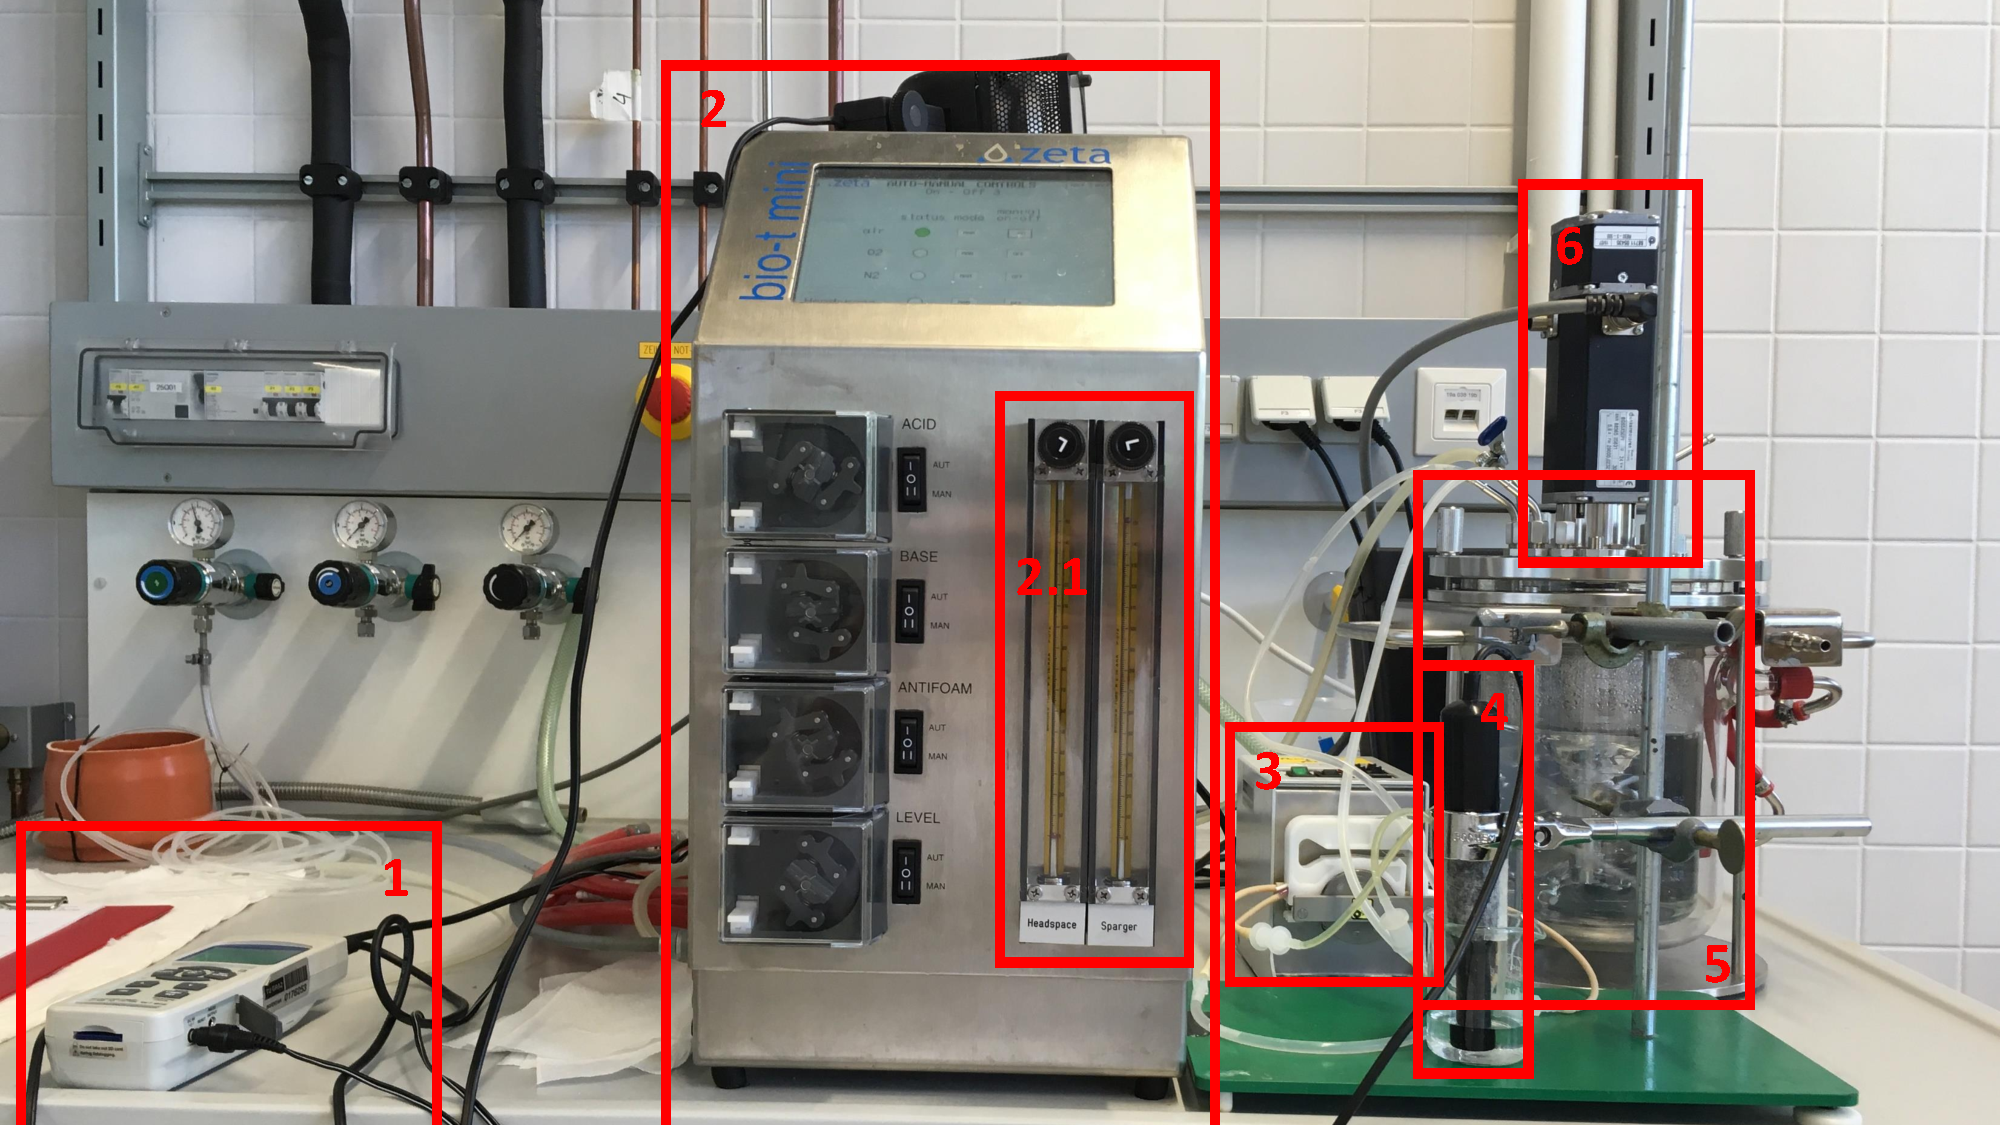
\includegraphics[width=0.8\textwidth]{Graphics/Versuchsaufbau_nummeriert.pdf} 
\caption[Versuchsaufbau am Labortag ]{Versuchsaufbau am Labortag | 1. Datalogger $\ch{O2}$-Sonde; 2. Steuereinheit \textit{bio-t mini}; 2.1. Durchflussmesser; 3. Schlauchquetschpumpe; 4. $\ch{O2}$-Sonde mit Becherglas (mit Stativ befestigt); 5. Versuchsreaktor mit Rührer; 6. Motor (magnetgekuppelt) }
\label{Versuchsaufbau}
\end{figure}
\noindent

\begin{figure}[H]
\centering
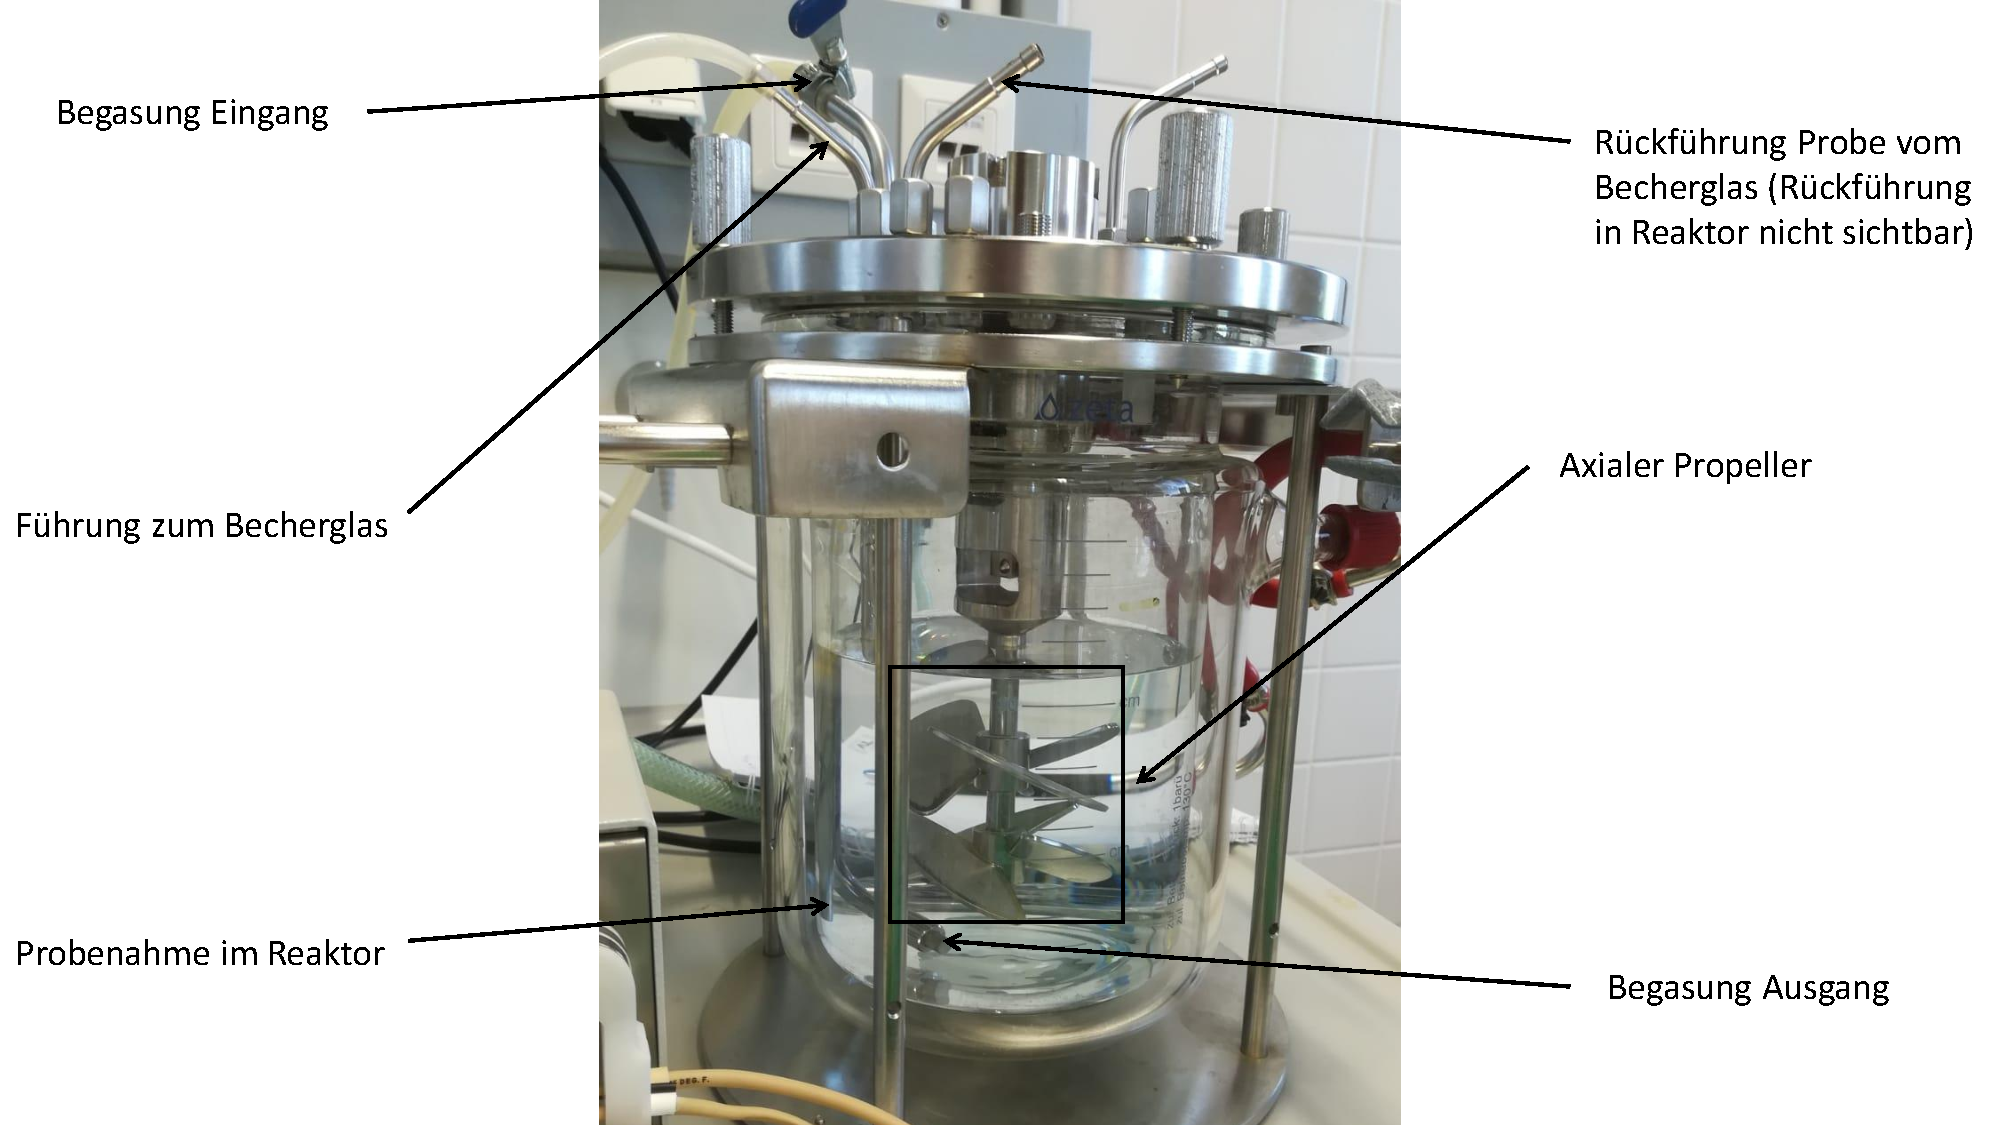
\includegraphics[width=0.8\textwidth]{Graphics/Reaktor_detail.pdf} 
\caption{Detailaufnahme des verwendeten Reaktors}
\label{Reaktor_detail}
\end{figure}
\noindent

\begin{figure}[H]
\centering
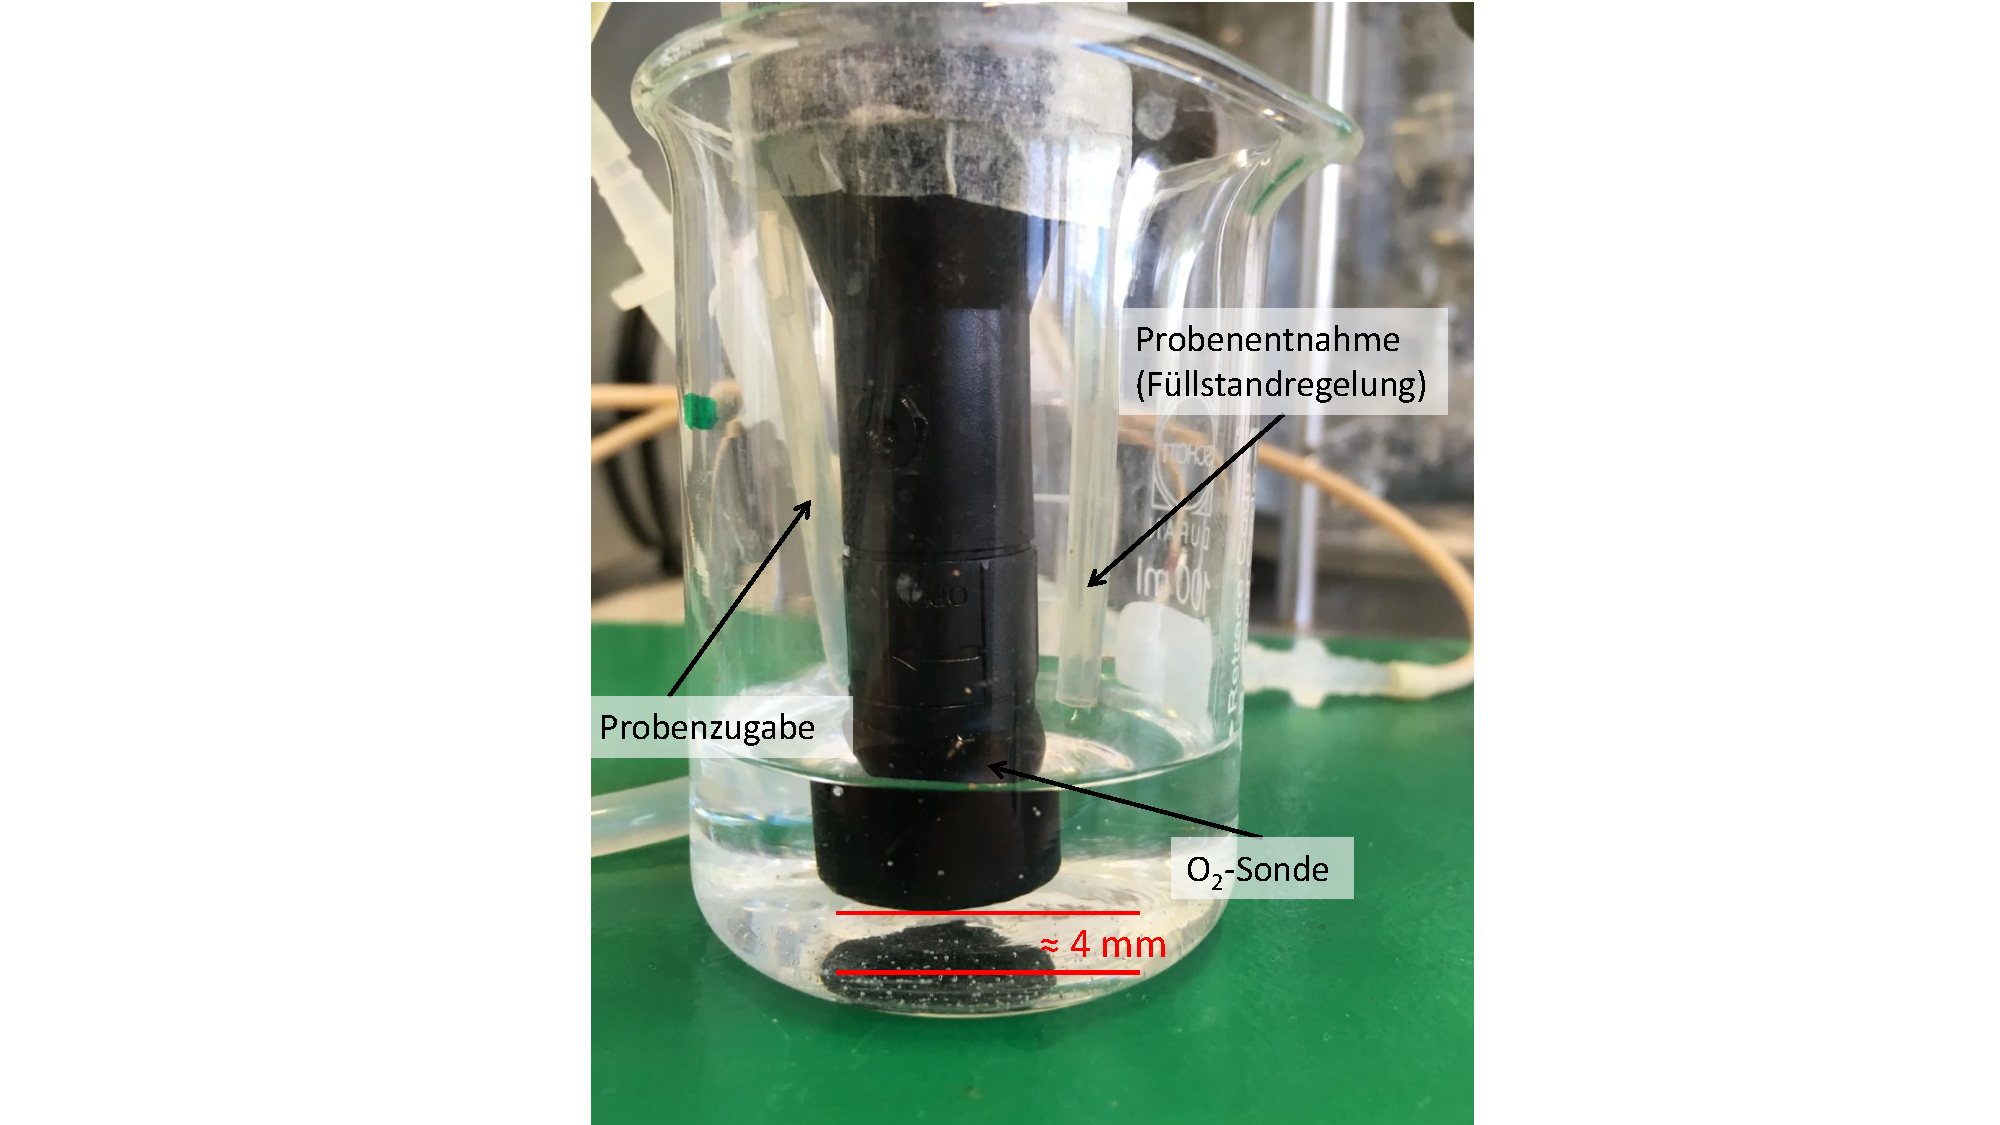
\includegraphics[width=1\textwidth]{Graphics/Sonde_Detail_beschriftet.pdf} 
\caption{Detail $\ch{O2}$-Sonde Abstand vom Becherglasboden}
\label{Sonde_Detail}
\end{figure}
\noindent


\chapter{Eingangsberechnungen}

Zum Zwecke der Versuchsvorbereitung werden Vorberechnungen durchgeführt, welche eine Abschätzung der benötigten Zeit zum Erreichen der Sättigungskonzentration an Sauerstoff als Ziel haben. In einem ersten Schritt wird dazu das Volumen des verwendeten Reaktors bestimmt. Eine grobe bemaßte Darstellung findet sich in Abbildung \ref{fig:masseReactor} (angelehnt an \cite{Labor_Skript}). Um das Volumen der Flüssigkeit und nicht des Behälters zu ermitteln wird angenommen, dass der Reaktor zu 80\,$\%$ befüllt ist. Folglich ist das Reaktorvolumen:

\begin{figure}[H]
\centering
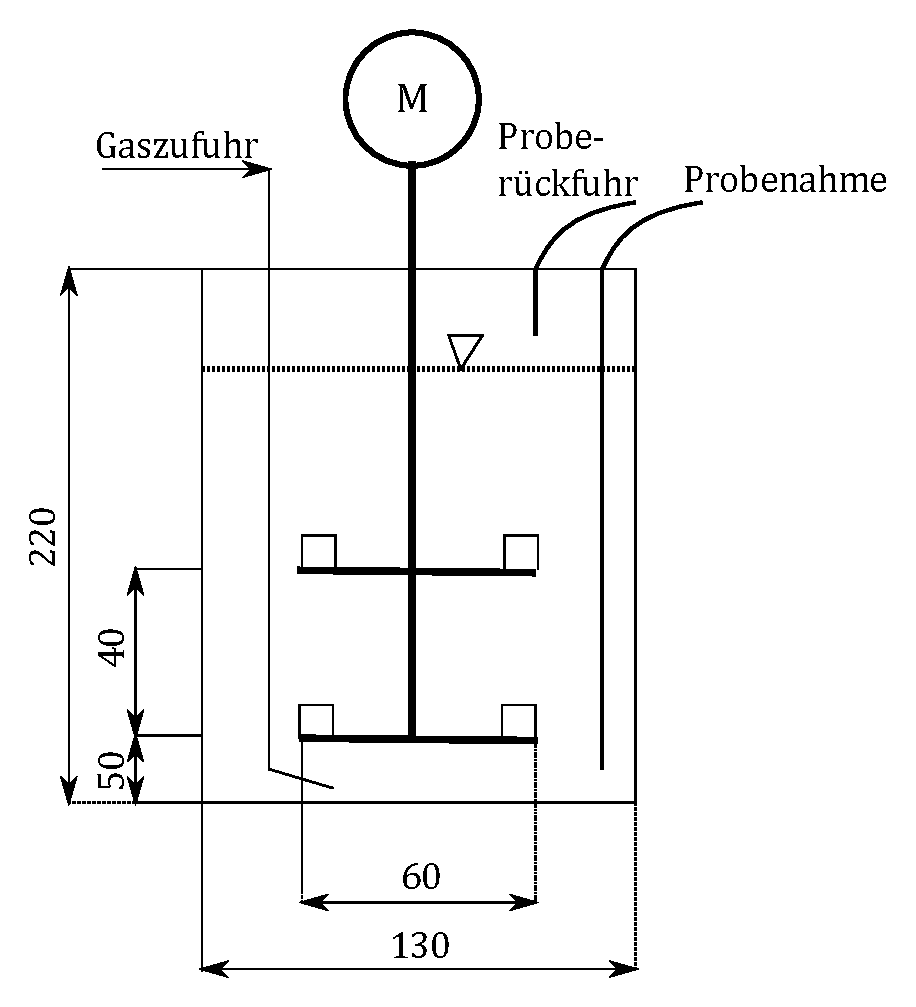
\includegraphics[width=0.6\textwidth]{Graphics/SkizzeReaktor.pdf}
\caption{Schematische Darstellung des Reaktors}[Maße in mm]
\label{fig:masseReactor}
\end{figure}
\noindent

\begin{equation}
 V_{R,fluid} = \frac{D^2 \cdot \pi}{4} \cdot L \cdot 0,8 = \frac{0,13^2 \cdot \pi}{4} \cdot 0,22 \cdot 0,8 = 2,34 \cdot 10^{-3}\,\m^3  
\end{equation}
\noindent
In einem nächsten Schritt muss die Henry-Konstante für Sauerstoff $O_2$ kalkuliert werden, um das Einstellen des Gleichgewichts zwischen Druck über der Flüssigkeit (Dampfdruck) und der Konzentration in der Flüssigkeit zu quantifizieren. Hierfür wird Gleichung (\ref{eq:henrykonstante}) laut \cite{Labor_Skript} herangezogen, wobei sich als Einheit für diesen polynomialen Fit bar ergibt und Raumtemperatur angenommen wird.

\begin{equation}
\label{eq:henrykonstante}
 H_{\ch{O2}} = -4,2857 \cdot T^2 + 3194,3 \cdot T - 525314 = 44801,388\,\text{bar}
\end{equation}
\noindent
Somit kann der Molenbruch im Gleichgewicht $x^{*,\infty}$ ermittelt werden, sprich jener Molenbruch der sich einstellt wenn zwischen der gelösten und der gasförmigen Phase an $O_2$ laut der Reaktionsgleichung $O_{2,(aq)} \leftrightharpoons O_{2, (g)}$ der Gleichgewichtszustand erreicht wird. Es muss also das Gleichgewicht zwischen der Luft über der Flüssigkeit mit $21\,\%$ Sauerstoffgehalt und dem Sauerstoff in der Flüssigkeit beachtet werden.

\begin{equation}
    x^{*,\infty} = \frac{0,21}{H_{\ch{O2}}} = \frac{0,21\,\text{bar}}{44801,388\,\text{bar}} = 4,69 \cdot 10^{-6}
\end{equation}
\noindent
Folglich kann die Konzentration an Wasser im Reaktorvolumen in mol$\cdot$l$^{-1}$ unter Berücksichtigung der Dichte von $\rho_{W} = 1000\,\text{kg}\cdot \text{m}^{-3} = 1000\,\text{g}\cdot \text{l}^{-1}$ und der molaren Masse $M_W = 18$\,$\text{g}\cdot \text{mol}^{-1}$ berechnet werden um in weiterer Folge die Gleichgewichtskonzentration des gelösten Sauerstoffs zu erhalten.

\begin{equation}
    c_w = \frac{\rho_{W}}{M_W} = \frac{1000}{18} = 55,44\,\frac{\text{mol}}{\text{l}}
\end{equation}
\noindent
Mithilfe der molaren Masse von Sauerstoff $M_{O_2} = 32$\,$\text{g}\cdot \text{mol}^{-1}$ kann die ermittelte Konzentration in $\text{mg}\cdot \text{l}^{-1}$ angegeben werden.
\begin{equation}
 c_{O_2}^* = c_w \cdot x^{*,\infty} = 55,44 \cdot 4,69 \cdot 10^{-6} = 2,60 \cdot 10^{-4}\,\frac{\text{mol}}{\text{l}} = 8,32\,\frac{\text{mg}}{\text{l}}
\end{equation}
\noindent
Da dieser Wert ein wenig unhandlich ist, wird zur besseren Vorstellung der übergehenden Gasmenge das Volumen angegeben, wobei die Konzentration im flüssigen Reaktorvolumen $V_{R,fluid}$ zur Berechnung der Stoffmenge herangezogen wird und die ideale Gasgleichung bei atmosphärischem Druck und Raumtemperatur zum Ermitteln des Sauerstoffvolumens verwendet wird.

%\todo{Felix Gasvolumen mit idealem Gas angeben}
\begin{equation*}
    c_{O_2}^* = \frac{N}{V} \rightarrow N_{O_2} = c_{O_2}^* \cdot V_{R,fluid} = 2,60\cdot10^{-4}\,\frac{\text{mol}}{\text{l}} \cdot 2,34\,\text{l} = 6,08\cdot10^{-4}\,\text{mol}
\end{equation*}
\begin{equation}
    p\cdot V = N\cdot R\cdot T \rightarrow V_{O_2} = \frac{N_{O_2} \cdot R \cdot T}{p_{atm}} = 0,14638\,\text{l}
\end{equation}
\noindent
Mit einem Volumen von $\approx$\,0,15\,l Sauerstoff kann eine bessere Vorstellung der gelösten Sauerstoffmenge erhalten werden.
\\
\\
Um nun das Ziel der Abschätzung der benötigten Zeit zur Sättigung zu erreichen, werden für eine erste Approximation ein $k_la$-Wert von 0,001\,$\text{s}^{-1}$ und eine Sättigung von 99\,$\%$ festgelegt. An dieser Stelle ist es wichtig zu erwähnen, dass für diese Kalkulation eine ideale Mischung im Bioreaktor und eine konstante Konzentration der Gasphase angenommen wird. Der Stofftransport wird durch die Newton´sche Transportgleichung beschrieben \cite{Labor_Skript}:

\begin{equation}
    \dot{n} \left[\frac{\text{mol}}{\text{m}^3 \text{s}}\right] = \frac{dc}{dt} = k_la \cdot (c^{*,\infty} - c^{\infty}) 
\end{equation}
\noindent
Durch Integration mittels Trennung der Variablen erhält man folgende Form:

\begin{equation}
\label{eq:integratednewton}
 k_la = \frac{ln\left(\frac{c^{*,\infty} - c^{\infty}_1 }{c^{*\infty} - c^{\infty}_2}\right)}{(t_2 - t_1)}   
\end{equation}
\noindent
Mit der Definition, dass die Konzentration zum Startzeitpunkt $t_1$ = 0\,s gleich $c^{\infty}_1$=0\,$\frac{\text{mol}}{\text{l}}$ ist, wird durch Umformen der Gleichung \ref{eq:integratednewton} die Zeit zur 99\,$\%$igen Sättigung in einem letzten Schritt ermittelt.

\begin{equation}
    t_{sättigung} = \frac{ln\left(\frac{c^{*}_{O_2}}{c^{*}_{O_2}-c^{\infty}_1}\right)}{k_la} = 76,75\,\text{min}
\end{equation}
\noindent
Somit kann die benötigte Zeit für durchzuführende Versuche abgeschätzt und mit ca. 77\,min festgelegt werden. Die Versuchszeit während des eigentlichen Labortages konnte jedoch als geringer (zwischen 20 und 40 Minunten) festgestellt werden, da sich der $k_la$-Wert während des Labortages als höher herausstellte. 

\chapter{Versuchsdurchführung}
\label{sec:versuchsdurchfuehrung}

%Zur praktischen Durchführung der Versuche wird in einem ersten Schritt der Reaktor mit ca. 1,5\,l Leitungswasser befüllt und der Reaktordeckel mit den Schlauch- und Steckanschlüssen und dem zweistufigen Propellerrühr auf den Behälter geschraubt. Zum Sättigen des Wassers benötigte Druckluft wird aus dem hausinternen Netz bezogen, reiner Stickstoff kommt aus Gasflaschen. Beide Leitungen werden aufgedreht. Zur Überwachung der Gaszufuhr und des Gasdrucks wird die Steuereinheit \textit{Bio-T Mini} eingeschaltet und das benötigte Rotameter zur Durchflussmessung überprüft. 

Im Rahmen der experimentellen Ermittlung des $k_la$-Wertes werden Versuche laut Tabelle \ref{Versuche} durchgeführt. Die Berechnung des Gasdurchflusses während der einzelnen Experimente ist im Folgenden in diesem Kapitel ersichtlich. Die genauen Werte für die Berechnung befinden sich im Anhang. 


\begin{table}[H]
\caption{Einstellungen der versch. Versuche}
\centering
\begin{tabular}{ccccc}
\toprule 
$\#$ Versuch&Rührerdrehzahl&Höhenstand &\multicolumn{2}{c}{Gasdurchfluss}\\
-&$\nicefrac{\text{U}}{\min}$&mm&$\nicefrac{\text{l Luft}}{\text{h}}$&$\nicefrac{\text{l}\;\ch{N2}}{\text{h}}$\\
\midrule
1&450&150&9,17&9,32\\
2&300&150&8,91&9,06\\
3&450&100&4,81&4,90\\
\bottomrule
\end{tabular}
\label{Versuche}
\end{table}
\noindent
mit 
\begin{itemize}
    \item $T_{ref} = 20\,^\circ\text{C}$
    \item $p_{ref} = 1,01325\,\text{bar}$
    \item $\rho_{ref} = 1,205218\,\text{kg}\cdot\text{m}^{-3}$
\end{itemize}\label{Referenzparamter}

Nachdem der Versuchsaufbau abgeschlossen ist wird zuerst das im Reaktor befindliche Leitungswasser einmal bei einer Rührerdrehzahl von $N=450\,\text{U} \cdot \text{min}^{-1}$ und einem Luftvolumenstrom von 150\,mm laut Rotameteranzeige gesättigt. Durch eine Kalibrationsfunktion lässt sich aus der Stellhöhe des Rotameters der Volumenstrom der Referenzwerte ermitteln. Die Kalibrationsfunktion ist in Quelle \cite{Labor_Skript} auf Seite 13 ersichtlich. Zur genaueren Veranschaulichung ist die Funktion in Abbildung \ref{KalibrationDurchfluss} dargestellt. Da auf dem Datenblatt die Werte für 150\,mm fehlen, wurde eine Extrapolierung durchgeführt. Die generierte Gleichung beläuft sich auf folgenden Zusammenhang mit einem Bestimmtheitsmaß nach \textit{\textit{Excel}} mit $R^2=1$:

\begin{equation}
    Q_{ref} = 0,0003 \cdot H_{R}^2 + 0,013\cdot H_{R} + 0,9808
\end{equation}

Für eine Stellhöhe von $H_{R} = 150\,\text{mm}$ ergibt sich daher bei Referenzbedingungen:
\begin{equation}
    Q_{ref} = 0,0003 \cdot 150\,\text{mm}^2 + 0,013\cdot 150\,\text{mm} + 0,9808 \approx 9,68\,\frac{\text{l Luft}}{\text{h}}
\end{equation}

%\todo{Kalibration und Extrapolieren Gasvolumenstrom, auch gleich Erklärung Umrechnung auf Stickstoff}

\begin{figure}[H]
\centering
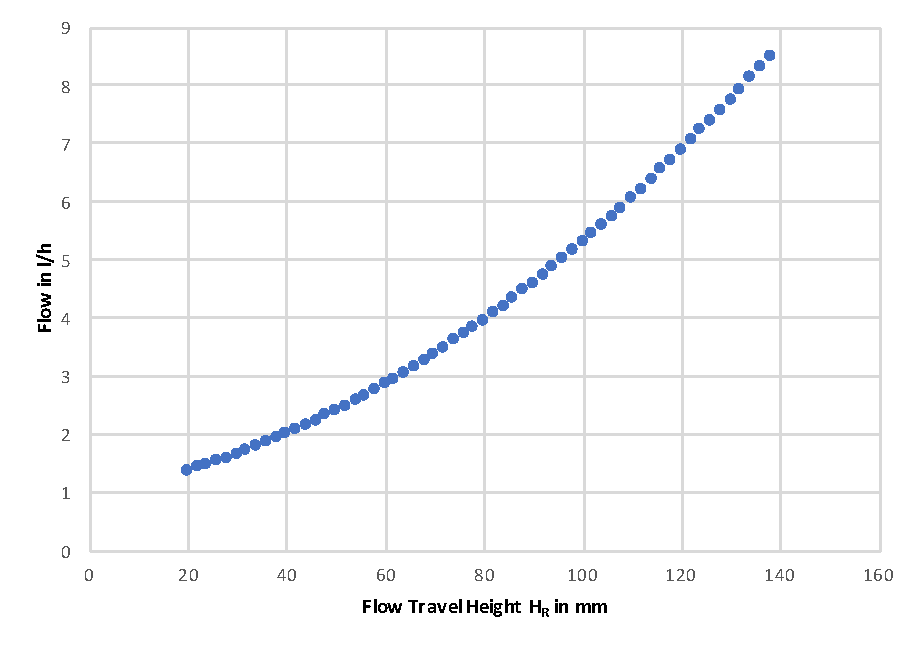
\includegraphics[width=0.8\textwidth]{Graphics/Flowrate.pdf}
\caption{Kalibrationsfunktion der Rotameter der Steuereinheit}[Daten laut Hersteller für Luft bei 20\,°C und 1\,atm]
\label{KalibrationDurchfluss}
\end{figure}
\noindent

Die Angabe des Gasvolumenstroms $\dot{G} = Q$ für Druckluft und Stickstoff erfolgt in mm Höhe des Rotameters. Eine Umrechnung kann mithilfe der Referenzparameter für Luft bei 20\,°C, 1,013\,bar und der resultierenden Dichte erfolgen (siehe Seite \pageref{Referenzparamter}). Die Berechnung des tatsächlichen Gasvolumenstroms für Luft und Stickstoff stützt sich daher auf folgende Vorgangsweise:

\begin{equation}
    \frac{Q_{ref}}{Q_{real}}=\sqrt{\frac{\rho_{real} \cdot T_{real} \cdot p_{ref}}{\rho_{ref} \cdot T_{ref} \cdot p_{real}}}
\end{equation}

Beispielhaft für den ersten Versuch ergibt sich für den Luftvolumenstrom folgender Wert. Die Parameter sind im Anhang ersichtlich:

\begin{equation}
    Q_{real}=\frac{9,68\,\frac{\text{l}}{\text{h}}}{\sqrt{\frac{2,362\,\frac{\kg}{\m^3} \cdot 22,47\,^\circ\text{C} \cdot 1,01325\,\text{bar}}{1,205218\,\frac{\kg}{\m^3} \cdot 20\,^\circ\text{C} \cdot 2\,\text{bar}}}}\approx9,17\,\frac{\litre}{\text{h}}
\end{equation}

Die Sättigung der flüssigen Phase erfolgt damit für die angegebenen Versuchsparameter. Es wird immer zuerst der Sauerstoff mit $\ch{N2}$ ausgetrieben und anschließend wieder eine Sättigung durchgeführt, folglich sind für jedes Experiment quasi zwei Sauerstoffkonzentrationsverläufe darstellbar. 
\\
\\
Im Anschluss an die erste Sättigung kann der erste Versuch mit Parametern laut Tabelle \ref{Versuche} begonnen werden, indem die Rührerdrehzahl am Control-Panel der Steuereinheit eingestellt wird und die Druckluftversorgung kontrolliert bzw. eingeschalten wird. Der Druck der zugeführten Luft (auch gültig für Stickstoffstrom) kann über ein Manometer an der Rückwand der Steuereinheit für alle Versuche auf $p=2\,\text{bar}$ geregelt werden, wobei simultan am Stellrad des Rotameters die geforderte Höheneinstellung und damit der Durchfluss justiert wird. Dabei ist darauf zu achten, dass als Schwebekörper in diesem Fall eine Kugel verwendet wird und als Referenz die horizontale Mitte der Kugel zu beachten ist. Während aller Experimente ist sicherzustellen, dass der Datenlogger der Sauerstoffsonde aktiv ist und die Schlauchquetschpumpe der unterschiedlich stark geklemmten Schläuche für die Probenahme auf maximalen Drehzahleinstellungen läuft.
\\
\\
Bei Versuch Nr. 1 wird also bei einer Rührerdrehzahl von 450\,$\text{U} \cdot \text{min}^{-1}$ und einem Rotameter-Höhenstand von 150\,mm der Sauerstoff ausgetrieben, wobei der erreichte Sauerstoff Konzentrationswert nach 40\,min mit 2\,$\text{mg} \cdot \text{l}^{-1}$ $\ch{O2}$ als Baseline definiert wird. Der vor dem Versuch erreichte Gleichgewichtszustand an gelöstem Sauerstoff wird als Referenzwert für die weiteren Versuche verwendet, sprich wenn diese Konzentration erreicht wird kann der Versuch als abgeschlossen angesehen werden. 
\\
\\
Nachdem also der vor den Versuchen erreichte Sättigungssauerstoff mit Stickstoff ausgetrieben wurde, wird der Gasdurchfluss von Stickstoff auf Druckluft umgestellt und die Manometer und Rotameter-Einstellungen justiert. Bei allen Versuchen wird die Zeit bzw. Dauer bis der Maximal- bzw. Minimalwert erreicht wird notiert, sprich die Daten erhalten einen Zeitstempel. Nachdem die Gleichgewichtskonzentration bei Versuch 1 sich einstellt, wird das Experiment abgeschlossen, der Datenlogger beendet die Aufzeichnung und die Daten werden von der SD-Karte extrahiert und der Speicher formatiert um die Daten des anschließenden Versuchs in eine frische Datei einzulesen. 
\\
\\
Im Rahmen des Sauerstoffsättigungsvorgangs wird zum Zwecke der Ermittlung der durchschnittlichen Blasengröße bei schwarzem Hintergrund mit Belichtung des Reaktors eine Fotoserie erstellt, wobei für die Auswertung der Blasengröße als Bezugsgröße die Dicke des Propellerrühers verwendet wird, welche manuell mit ca. 2\,mm gemessen wird. 
\\
\\
Im Anschluss an den neuen Datenlogging-Vorgang wird zuerst für ca. 4\,min noch mit dem Umstellen der Rührerdrehzahl und des Gasvolumenstroms gewartet. Mit den neuen Parametern für Versuch Nr. 2 laut Tabelle \ref{Versuche} werden die oben angeführten Schritte wiederholt. 
\\
\\
Während den Versuchen fällt auf, dass die zu Beginn erreichte Maximalkonzentration nicht wieder erreicht wird, nach einer angemessen Zeitspanne wird trotz geringer Schwankungen des maximalen Wertes der Versuch als abgeschlossen betrachtet. Selbiges gilt auch für den Austreibungsvorgang. 
\\
\\
Schlussendlich wird nach dem Fahren der drei Versuche die Anlage wieder abgebaut. Zuerst wird der Propellerrührer abgeschaltet, anschließend die Gaszufuhr abgedreht und die Probenahme abgeschaltet. Der Reaktor kann auf gleiche Weise wie er montiert wurde wieder demontiert und die Flüssigkeit entsorgt werden.

\chapter{Ergebnisse}

\section{Gemessene Konzentrationsverläufe}

In Abbildung \ref{cmessung} sind die gemessenen Konzentrationsverläufe für die drei durchgeführten Versuche dargestellt. Aus den Verläufen werden Intervalle ausgewählt, welche zur Berechnung des $k_la$-Wertes mittels Regression verwendet werden. In den blauen Bereichen wird der $k_la$-Wert für das Austreiben des Sauerstoffs ermittelt, und in den roten Bereichen für das Begasen.\\
\\
Die richtige Begrenzung des Berechnungs-Bereiches spielt eine wichtige Rolle. Der Start sollte möglichst an dem Punkt liegen, an dem der Abfall bzw. Anstieg der Konzentration beginnt. Zum Ende des Berechnungsintervalles sollte sich die Konzentration möglichst konstant verhalten. Etwaige starke Schwankungen oder Konzentrationsabfälle sollten ausgegrenzt werden.

\begin{figure}[H]
\centering
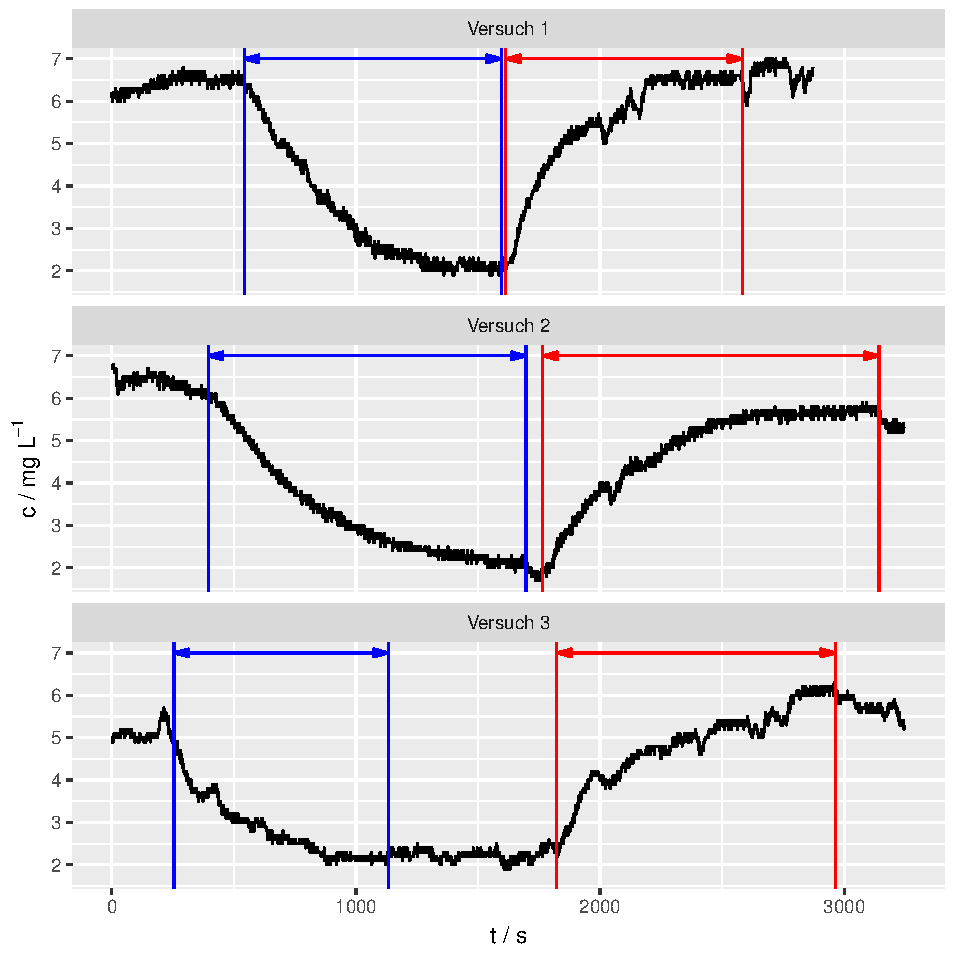
\includegraphics[width=1\textwidth]{Graphics/test.pdf} 
\caption[Gemessene Konzentrationsverläufe]{Gemessene Konzentrationsverläufe mit Berechnungsintervallen}
\label{cmessung}
\end{figure}
\noindent
Es kann also in Abbildung \ref{cmessung} der Zeitpunkt bei dem der Austreibungsvorgang mit $\ch{N2}$ beginnt beim linken Startpunkt der blauen Bemaßung festgestellt werden und der Beginn des Sättigungsvorgangs beim Start des linken Endes der roten Bemaßung. Die Wahl der Zeitpunkte für die Berechnung wird beispielsweise bei Versuch 1 derart begründet, dass die starken Schwankungen am Ende bei ca. 2800-300\,s für die weitere Berechnung des $k_la$-Wertes nicht hilfreich wären und damit ausgegrenzt werden. Die Konzentration an $\ch{O2}$ sinkt bei allen Versuchen beim Austreiben auf den Baseline-Wert von ca. 2\,mg$\cdot$l$^{-1}$. Dennoch fällt auf, dass dieser Wert bei den Versuchen zu unterschiedlichen Zeitpunkten erreicht wird, wie z.B. bei Versuch 2 erst nach ca. 1800\,s. Der Anstieg der gelösten Sauerstoffkonzentration ist beim ersten Versuch am größten bis zu einem maximalen Wert von ca. 7\,mg$\cdot$l$^{-1}$, wobei dieser Wert bei Versuch 2 und 3 nicht mehr erreicht wird.

\section{Ermittelte $k_la$-Werte}
\label{sec:kla}

Für die Ermittlung des $k_la$ kommen die Gleichungen für die Konzentration in Abhängigkeit der Zeit beim Aufsättigen und Austreiben zum Einsatz:

\begin{equation}
\label{eq:csaettigen}
    c_i^\infty(t) = c_i^{*,\infty} - \frac{c_i^{*,\infty}}{\exp\left(k_La \cdot t\right)}
\end{equation}

\begin{equation}
\label{eq:caustreiben}
    c_i^\infty(t) = \frac{c_{Start}}{\exp\left(k_La \cdot t\right)}
\end{equation}

Wobei $c_i^\infty(t)$ der Konzentration zum Zeitpunkt $t$ in unendlicher Entfernung der Phasengrenze (also im Bulk) entspricht. $c_i^{*,\infty}$ ist die Gleichgewichts-/Sättigungskonzentration.
Desweiteren wird das Bestimmtheitsmaß $R^2$ benötigt:

\begin{equation}
    R^2 = 1 - \frac{\sum\left(y_i-\hat{y}_i\right)^2}{\sum\left(y_i-\bar{y}_i\right)^2}
\end{equation}

Die Bestimmung des $k_la$-Wertes wird mit \textit{Excel} durchgeführt. Dazu wird zu jeder gemessener Konzentration eine theoretische Konzentration mit den Gleichungen \ref{eq:csaettigen}/\ref{eq:caustreiben} berechnet. Dafür kann zu Beginn ein beliebiger $k_la$-Wert verwendet werden, in diesem Falle 0,001\,s$^{-1}$ um mit der Eingangsberechnung konsistent zu bleiben. Beim Aufsättigen startet der Konzentrationsverlauf bei 0\,mg\,l$^{-1}$, beim Austreiben konvergiert der Konzentrationsverlauf gegen 0\,mg\,L$^{-1}$. Die gemessenen Konzentrationsverläufe müssen daher noch modifiziert werden, da immer eine gewisse Grund-Konzentration (Baseline-Wert) vorhanden ist. Dazu wird von jeder gemessenen Konzentration die kleinste, im Berechnungsintervall gemessene Konzentration subtrahiert.\\
\\
Beim Aufsättigen wird die Sättigungskonzentration benötigt. Um diese zu erhalten wird aus den letzten \textasciitilde 200 Konzentrationswerten der Mittelwert gebildet. Für das Austreiben wird die Startkonzentration benötigt. Diese entspricht der maximalen Konzentration im Berechnungsgebiet (diese sollte gleichzeitig auch dem ersten gemessenen Konzentrationswert entsprechen).\\
\\
Mit den gemessenen Werten und den berechneten Werten des Modells kann nun $R^2$ berechnet werden. Mit Hilfe des \textit{\textit{Excel}}-Solvers wird der $k_la$-Wert variiert, um so $R^2$ zu maximieren. Die so gefundenen $k_la$-Werte sind in Tabelle \ref{tab:kla_R} aufgelistet.

% Table generated by \textit{Excel}2LaTeX from sheet 'daten_R'
\begin{table}[H]
  \centering
  \caption{ermittelte $k_la$-Werte mit Bestimmtheitsmaß}
    \begin{tabular}{cccc}
    \toprule
    Versuch \# & Vorgang & $k_la$ / s$^{-1}$   & $R^2$ \\
    \midrule
    \multirow{2}[1]{*}{1} & austreiben & 0,00306 & 0,9771 \\
          & aufsättigen & 0,00435 & 0,9656 \\
          \midrule
             \multirow{2}[2]{*}{2} & austreiben & 0,00231 & 0,9918 \\
          & aufsättigen & 0,00311 & 0,9784 \\
          \midrule
    \multirow{2}[1]{*}{3} & austreiben & 0,00385 & 0,9410 \\
          & aufsättigen & 0,00254 & 0,8931 \\

    
          \bottomrule
    \end{tabular}%
  \label{tab:kla_R}%
\end{table}%

Die folgenden Diagramme zeigen den Konzentrationsverlauf beim Austreiben und Aufsättigen für den ersten Versuch. Beim Aufsättigen ist zusätzlich zum Fit und der gemessenen Konzentration noch die berechnete Gleichgewichtskonzentration eingezeichnet. Zur Berechnung wurden die Konzentrationswerte ab $t = 600\,\s$ verwendet. Die Verläufe der anderen Versuche sind im Anhang ersichtlich. Zu betonen gilt, dass alle Versuche einen ähnlichen Kurvenverlauf zeigen, wobei der Fit des dritten Versuches die größte Abweichung zu den tatsächlich gemessenen Daten zeigt. Lediglich die Sättigungskonzentration ändert sich von Versuch zu Versuch.

\begin{figure}[H]
\centering
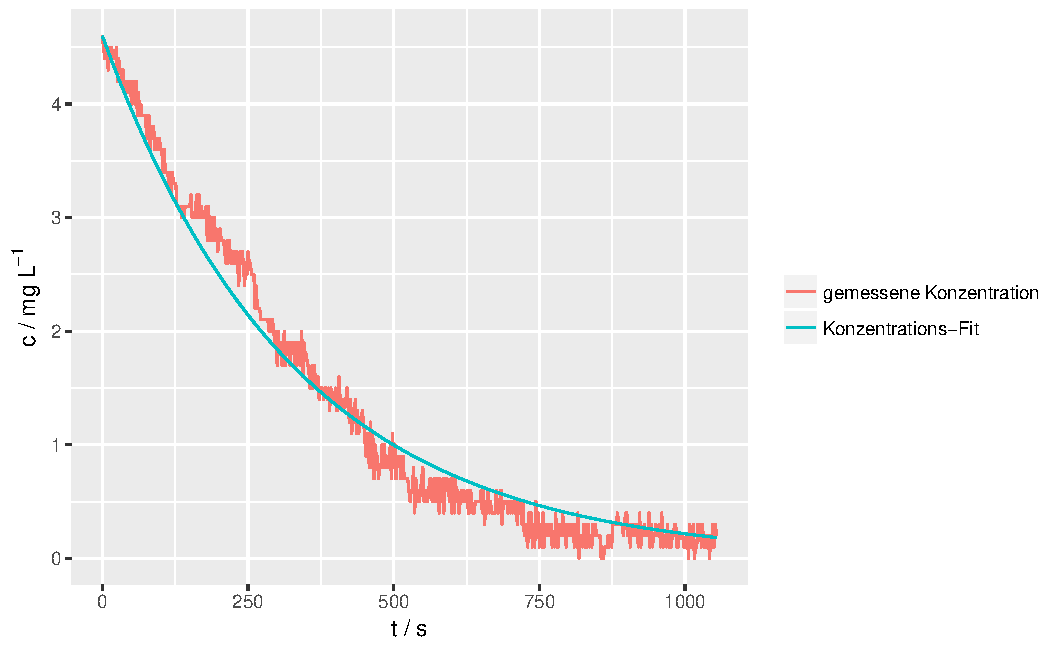
\includegraphics[width=1\textwidth]{Graphics/austreiben_versuch-1.pdf} 
\caption[Austreiben Versuch 1]{tatsächliche und gefittete Konzentration beim Austreiben - Versuch 1}
\label{fig:c_aus_versuch1}
\end{figure}
\noindent

\begin{figure}[H]
\centering
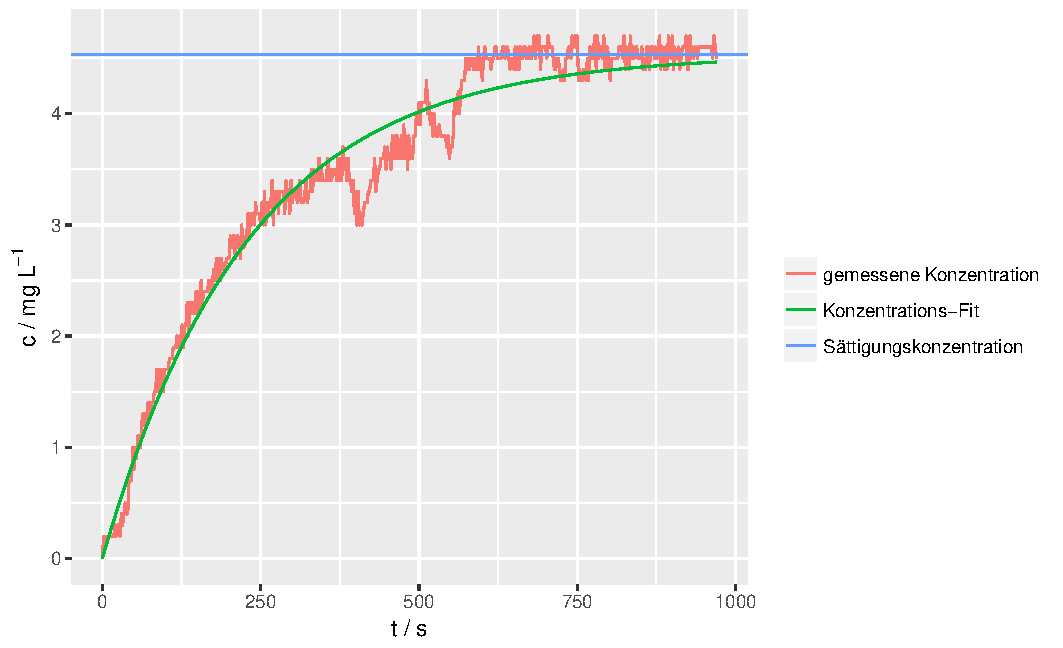
\includegraphics[width=1\textwidth]{Graphics/aufsaettigen_versuch-1.pdf} 
\caption{Aufsättigen Versuch 1}[tatsächliche und gefittete Konzentration beim Aufsättigen mit angenommener Gleichgewichtskonzentration - Versuch 1]
\label{fig:c_auf_versuch1_saett}
\end{figure}
\noindent



\section{Abschätzung des $k_l$-Wertes}

\subsection{Durchschnittliche Blasengröße und -anzahl}

Da beim Stoffdurchgangskoeffizient die spezifische Oberfläche oft nicht 
bekannt ist wird diese vom $k_l$-Wert mit $a_{spez}$ zum $k_la$-Wert 
zusammengefasst, welcher bei diesen Experimenten das erhaltene Ergebnis 
ist. Wird aber wie bei der Versuchsdurchführung erwähnt eine Fotoserie 
mit 40 Bildern pro Sekunde erstellt, kann mit einem Referenzmaß, in 
diesem Fall wird das Rührerblatt mit einer Dicke von 2\,mm gewählt, die 
durchschnittliche Blasengröße für 20 bis 25 zufällig verteilte Blasen 
gemessen werden. Dabei wird die Annahme getroffen, dass die Blasen 
annähernd kugelförmig sind, was sie eindeutig nicht sind, sondern stark 
verformt durch die durch den Rührer eingebrachten Scherkräfte und das 
Strömungsprofil. Für die Anzahl an ausgewerteten Bildern wird mit dem 
Gedankengang, dass bei einer Drehzahl von $450\,\text{U}\cdot\text{min}^{-1} =
7,5\,\text{U}\cdot\text{s}^{-1}$ und 40 Bildern pro Sekunde genau 5,7 Bilder eine Umdrehung des Rührers abbilden und diese Blasenverteilung und -größe sich
periodisch wiederholt, argumentiert. Analog gilt dies für 
$300\,\text{U}\cdot\text{min}^{-1}$. Eine beispielhafte Messung für den ersten Versuch ist in Abbildung \ref{fig:Messung} dargestellt. Die Fotoserie ist in 
Abbildung \ref{Fotoserie1} für eine Umdrehung (= 6 Bilder) ersichtlich. 
Die Serien für Versuch 2 und 3 sind im Anhang zu finden.


\begin{figure}[H]
    \centering
    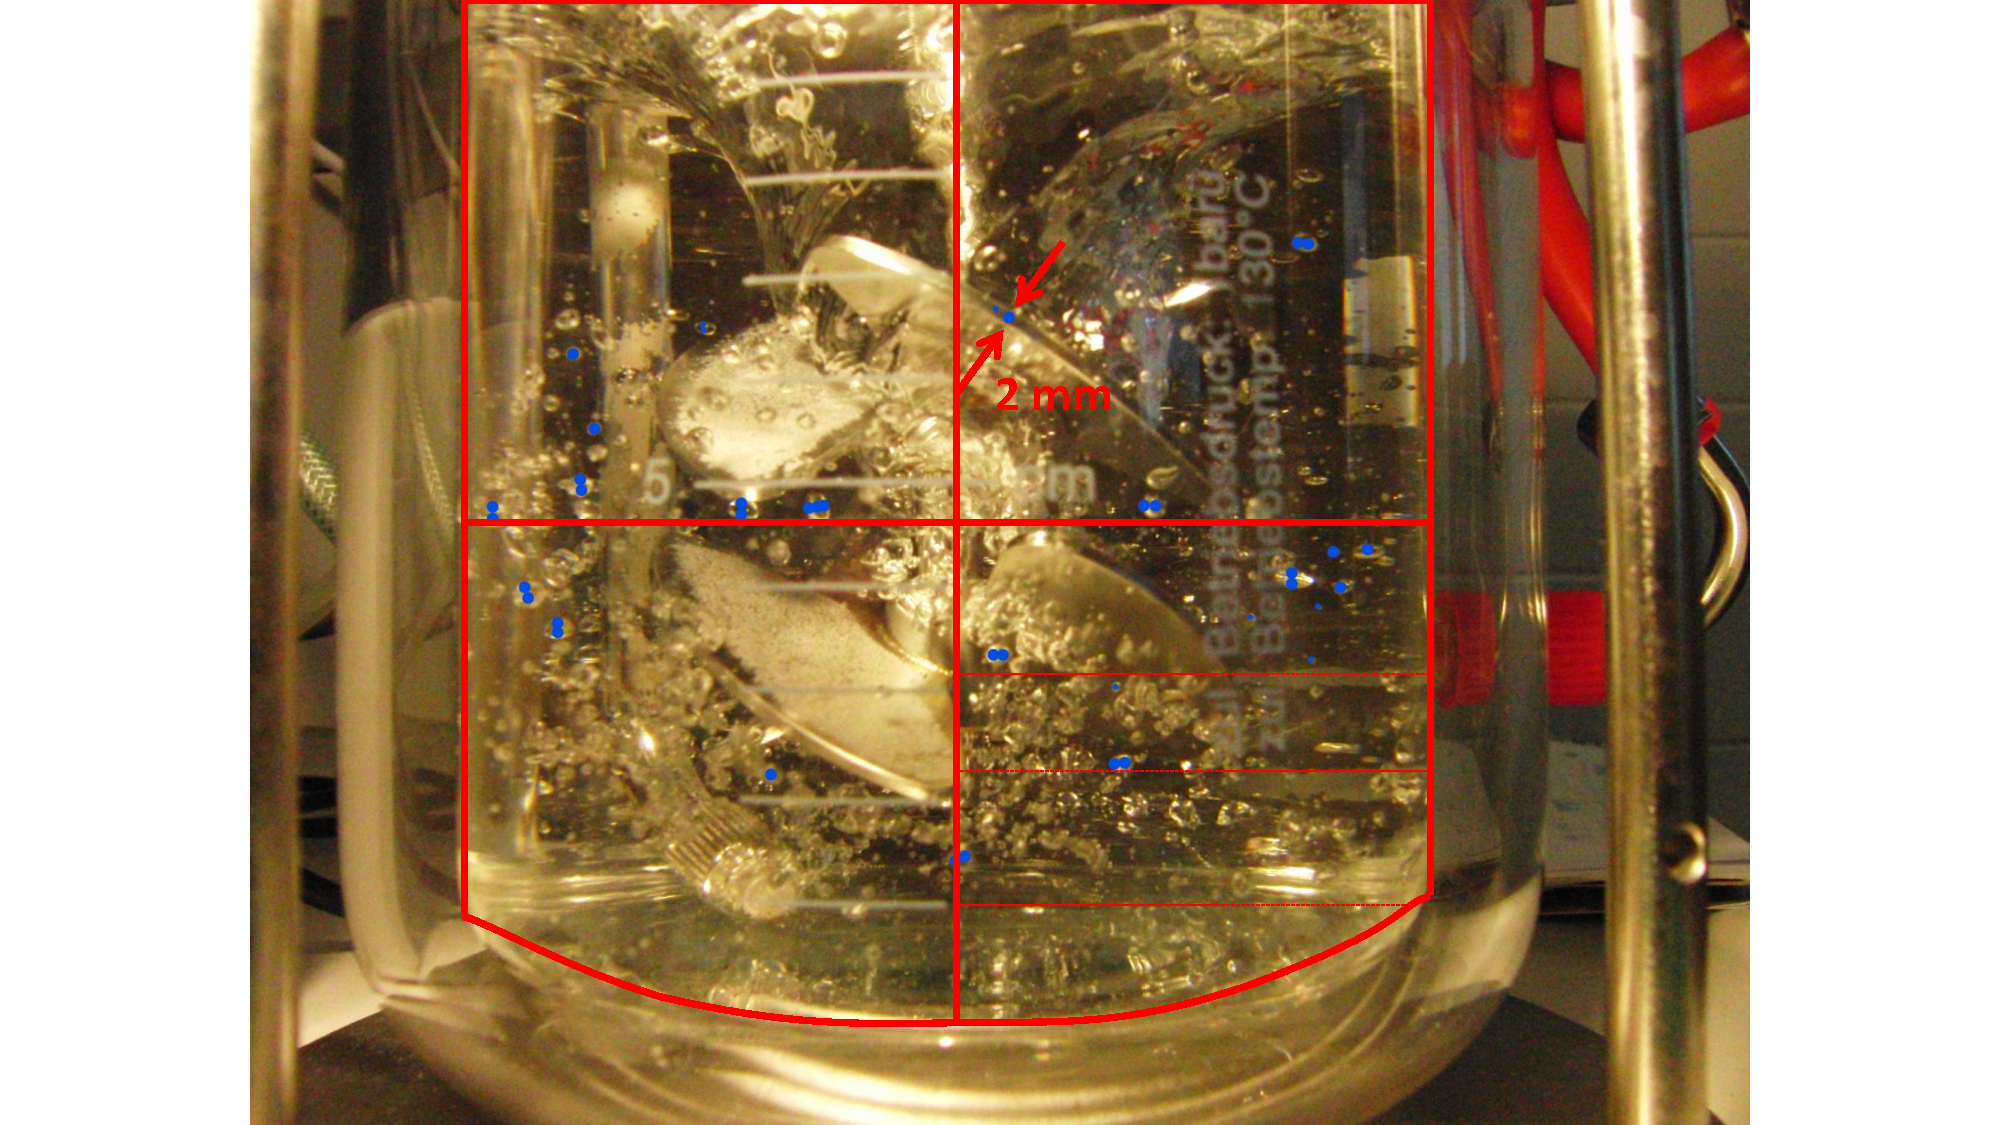
\includegraphics[width=0.8\textwidth]{Blasenmessung/Blasengrose_Versuch_1.pdf}
    \caption[Blasengrößenbestimmung mit Einteilung der Quadranten für Versuch 1]{Blasengrößenbestimmung durch Einzeichnen blauer Punkte mit Blattdicke als Referenz \& Einteilung der Quadranten für die Abschätzung der Blasenanzahl für Versuch 1}
    \label{fig:Messung}
\end{figure}

\begin{figure}[H]
\begin{center}
	\subfigure[Bild 1]{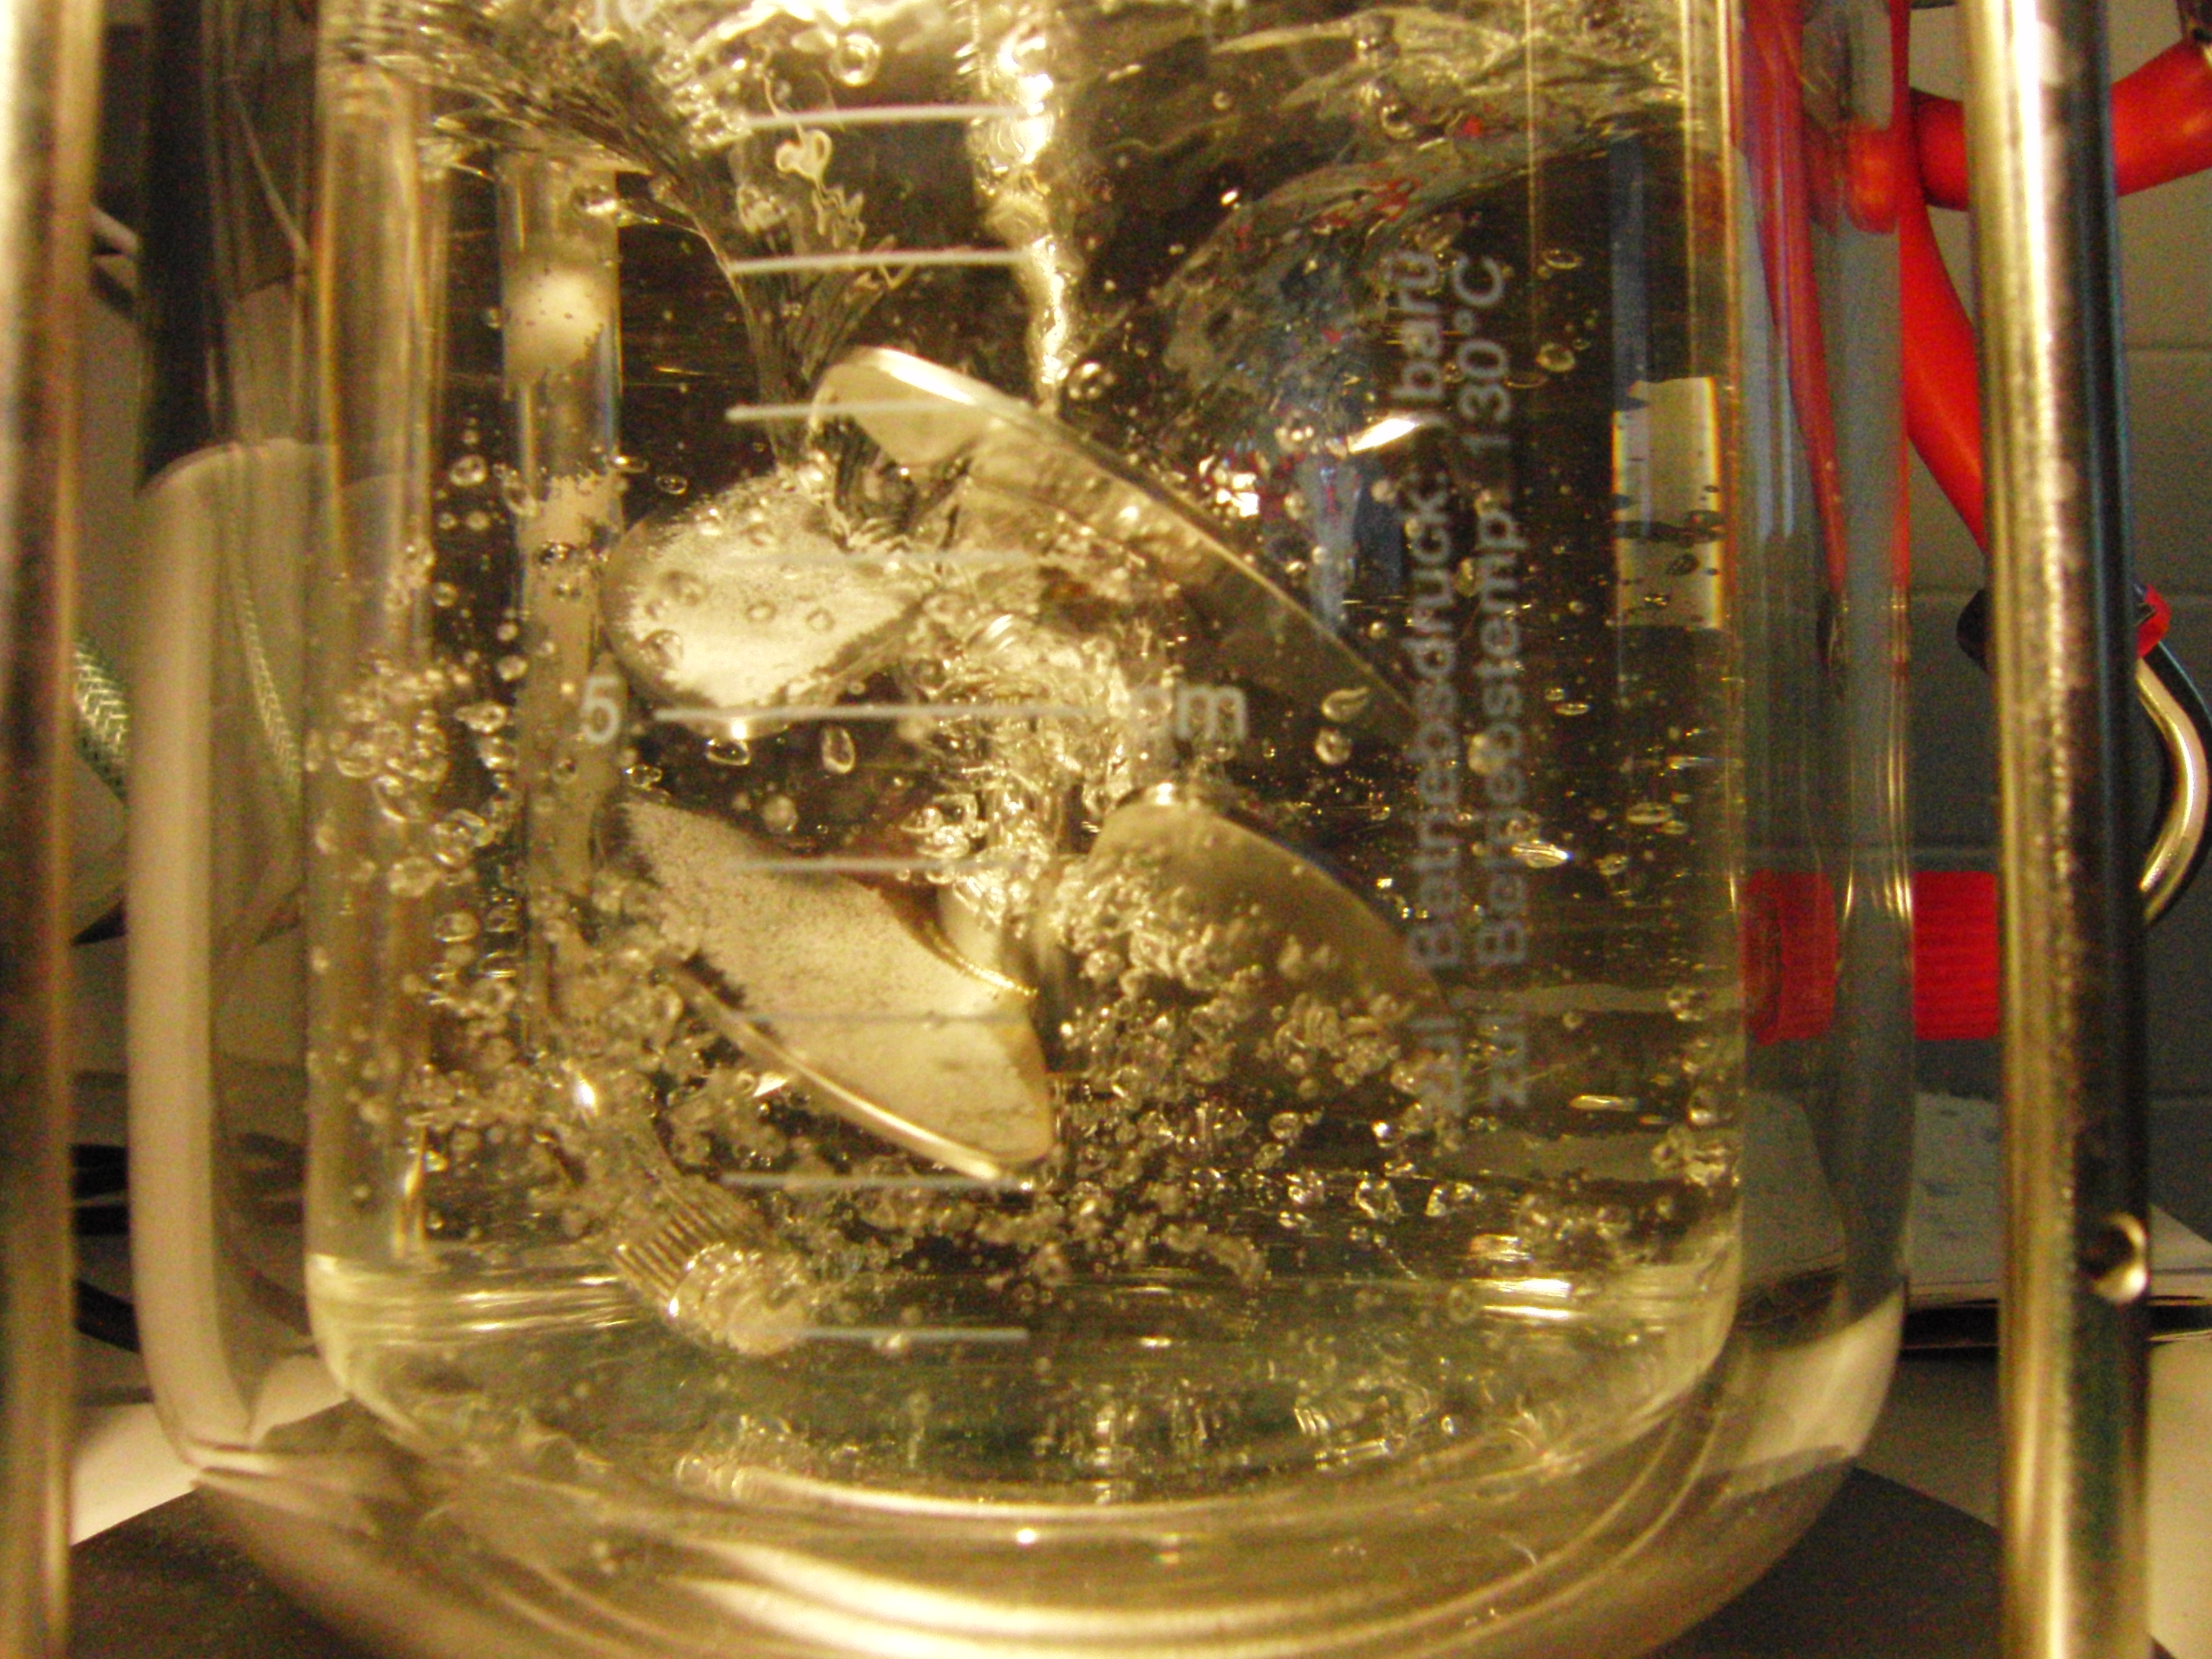
\includegraphics[height=4cm]{Blasenmessung/Versuch_1_1.JPG}}\label{blasengroesse1}
	\hspace{1cm}
	\subfigure[Bild 2]{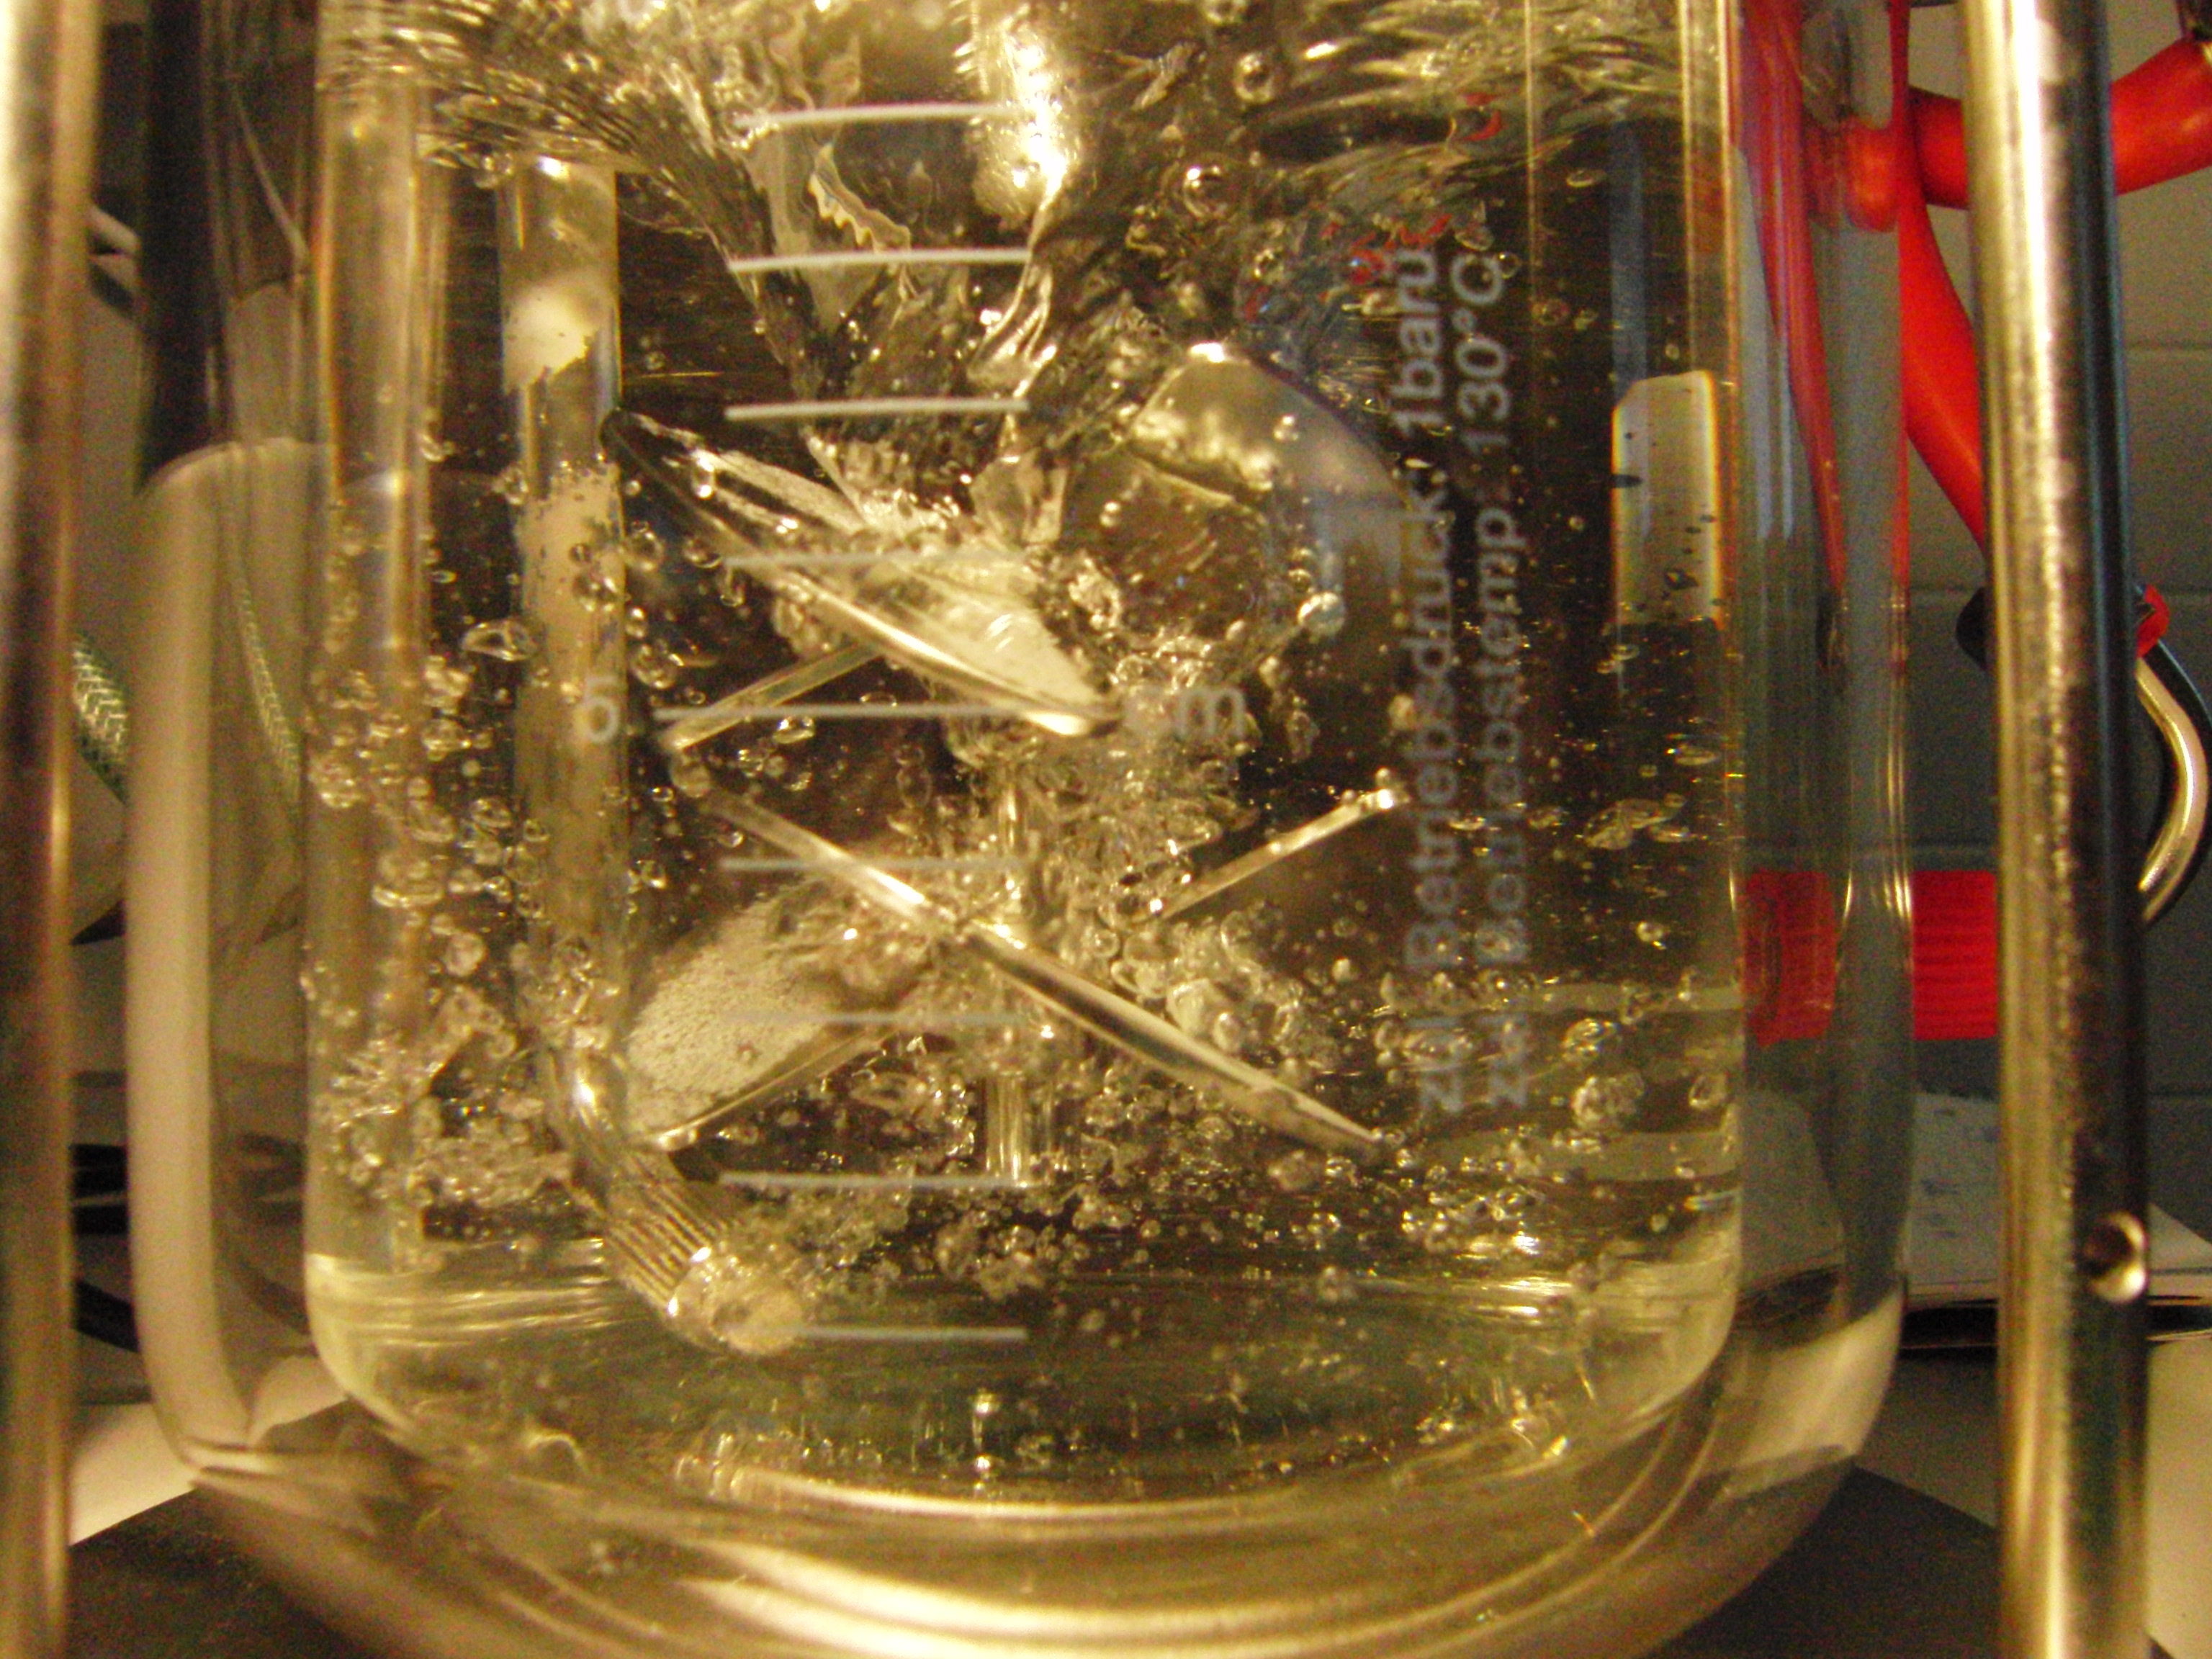
\includegraphics[height=4cm]{Blasenmessung/Versuch_1_2.JPG}}\label{blasengroesse2}
	\hspace{1cm}
	\subfigure[Bild 3]{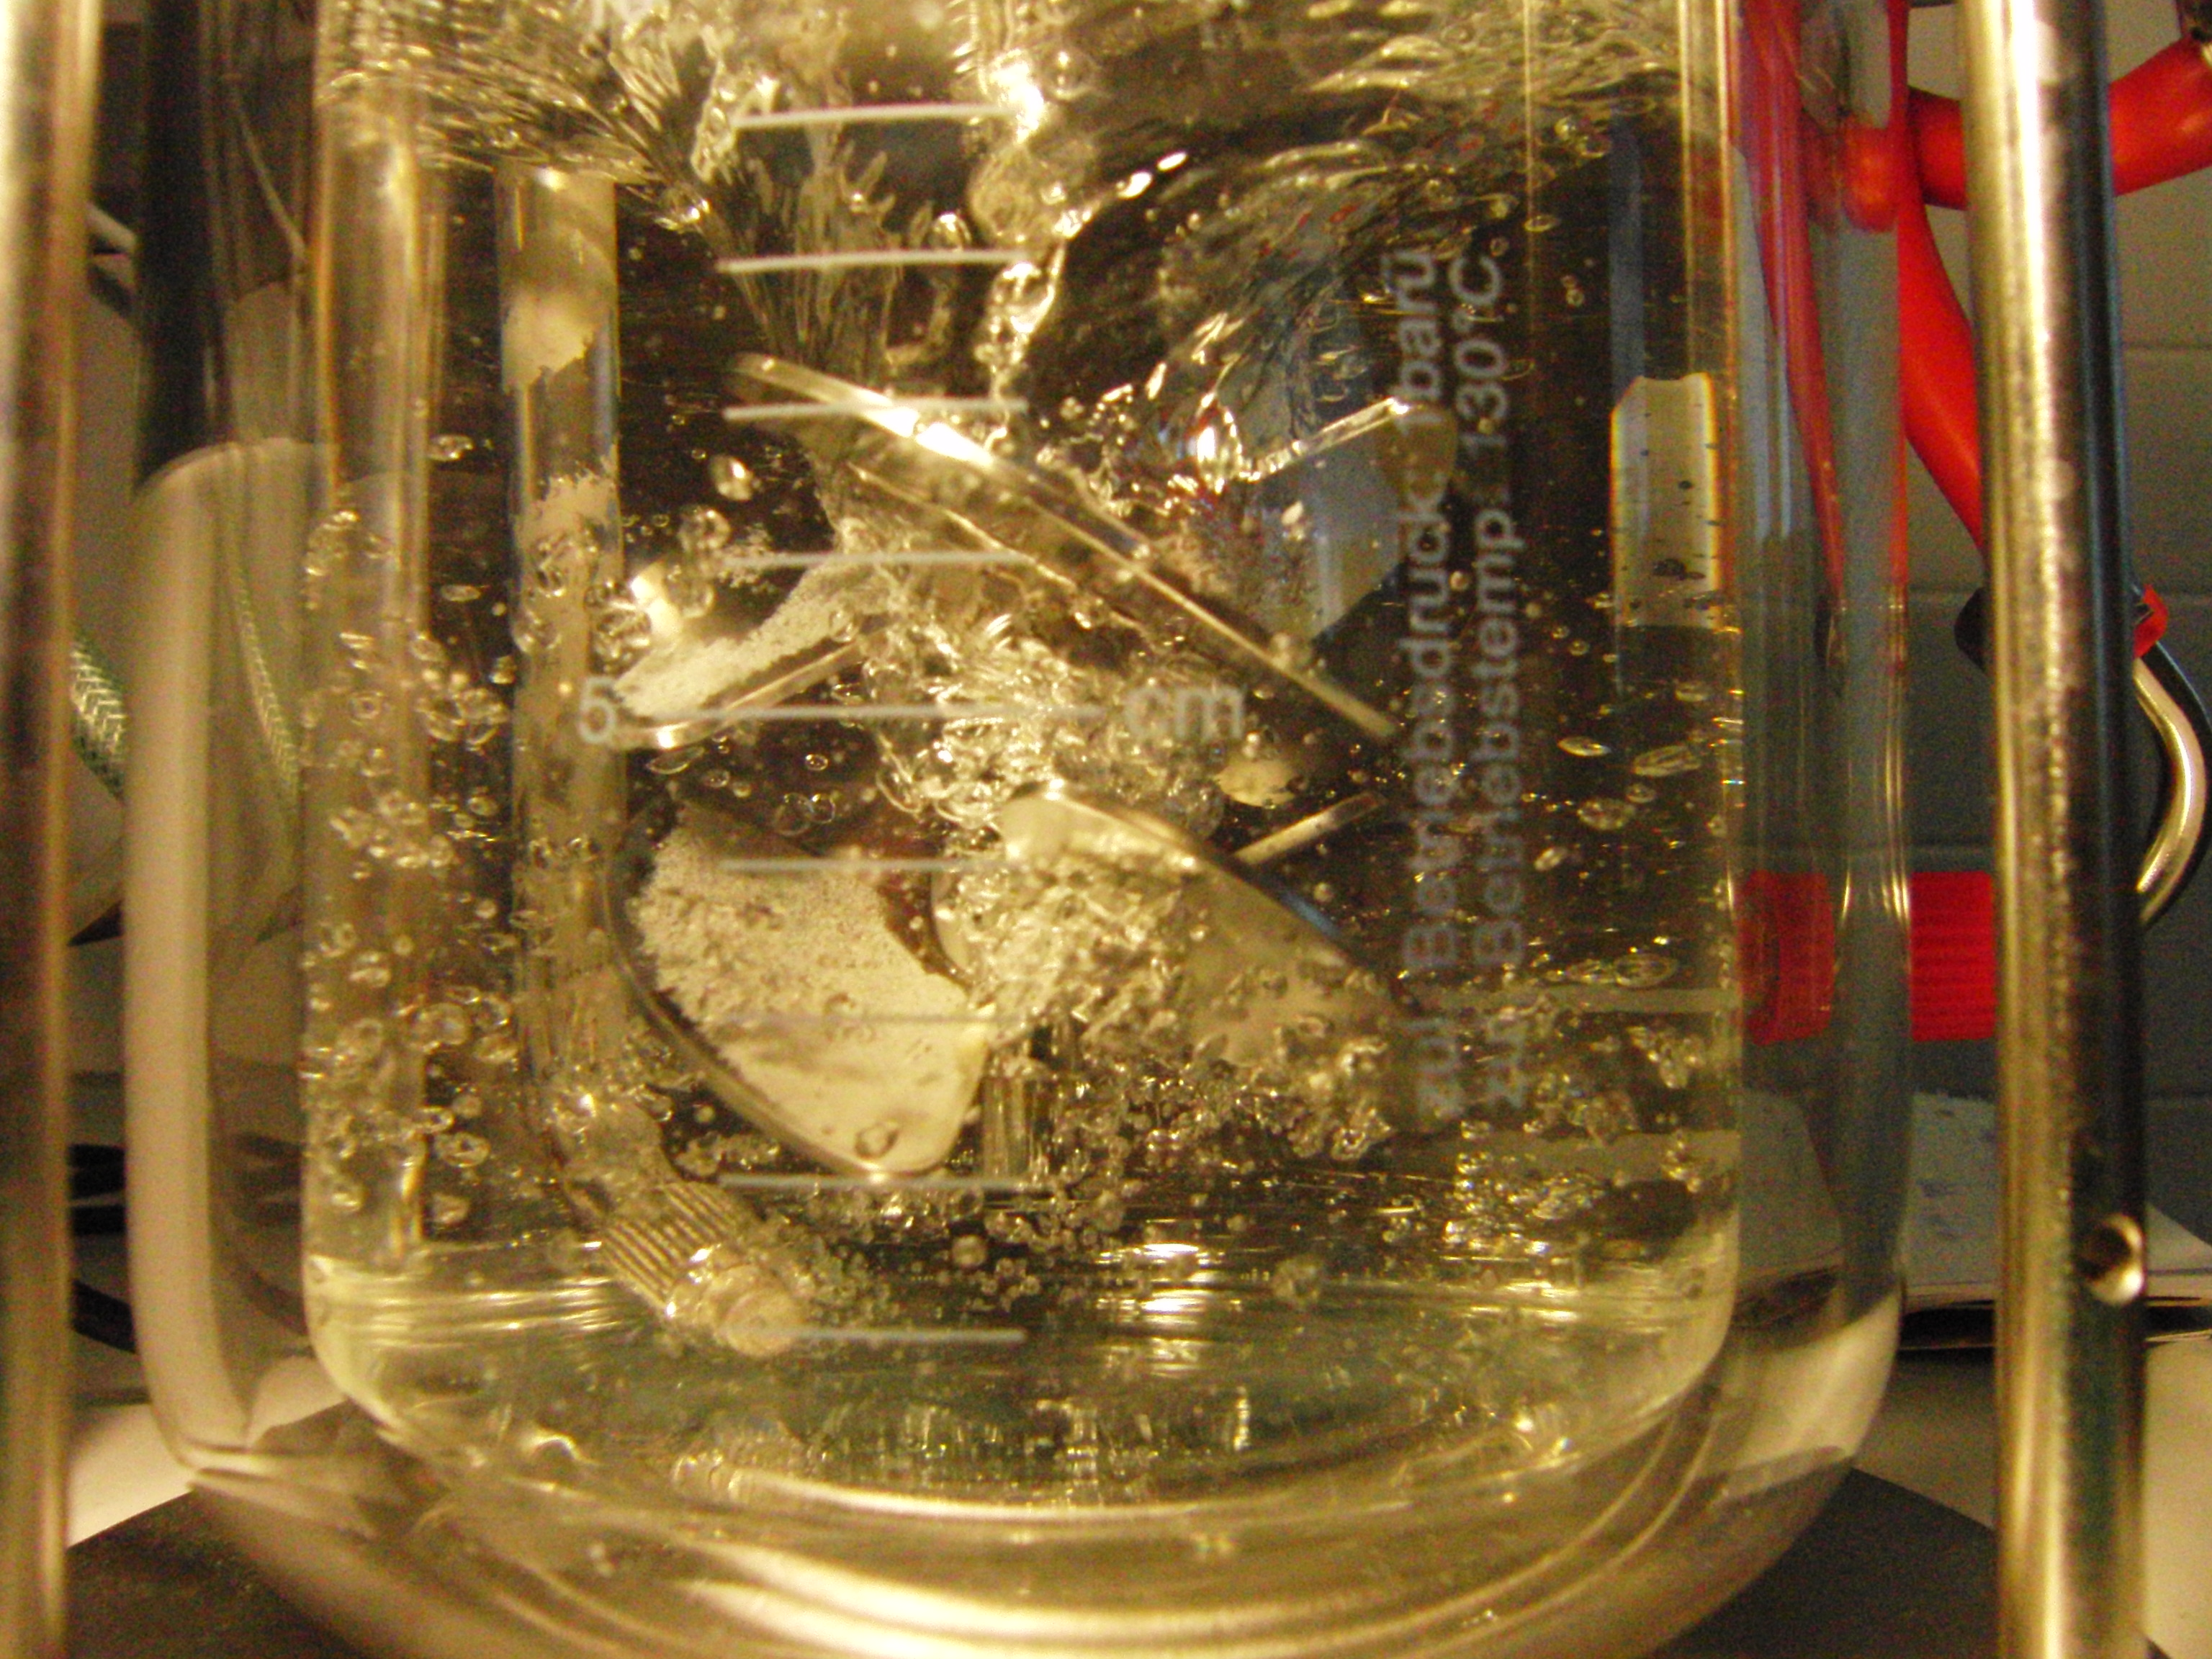
\includegraphics[height=4cm]{Blasenmessung/Versuch_1_3.JPG}}\label{blasengroesse3}
	\hspace{1cm}
	\subfigure[Bild 4]{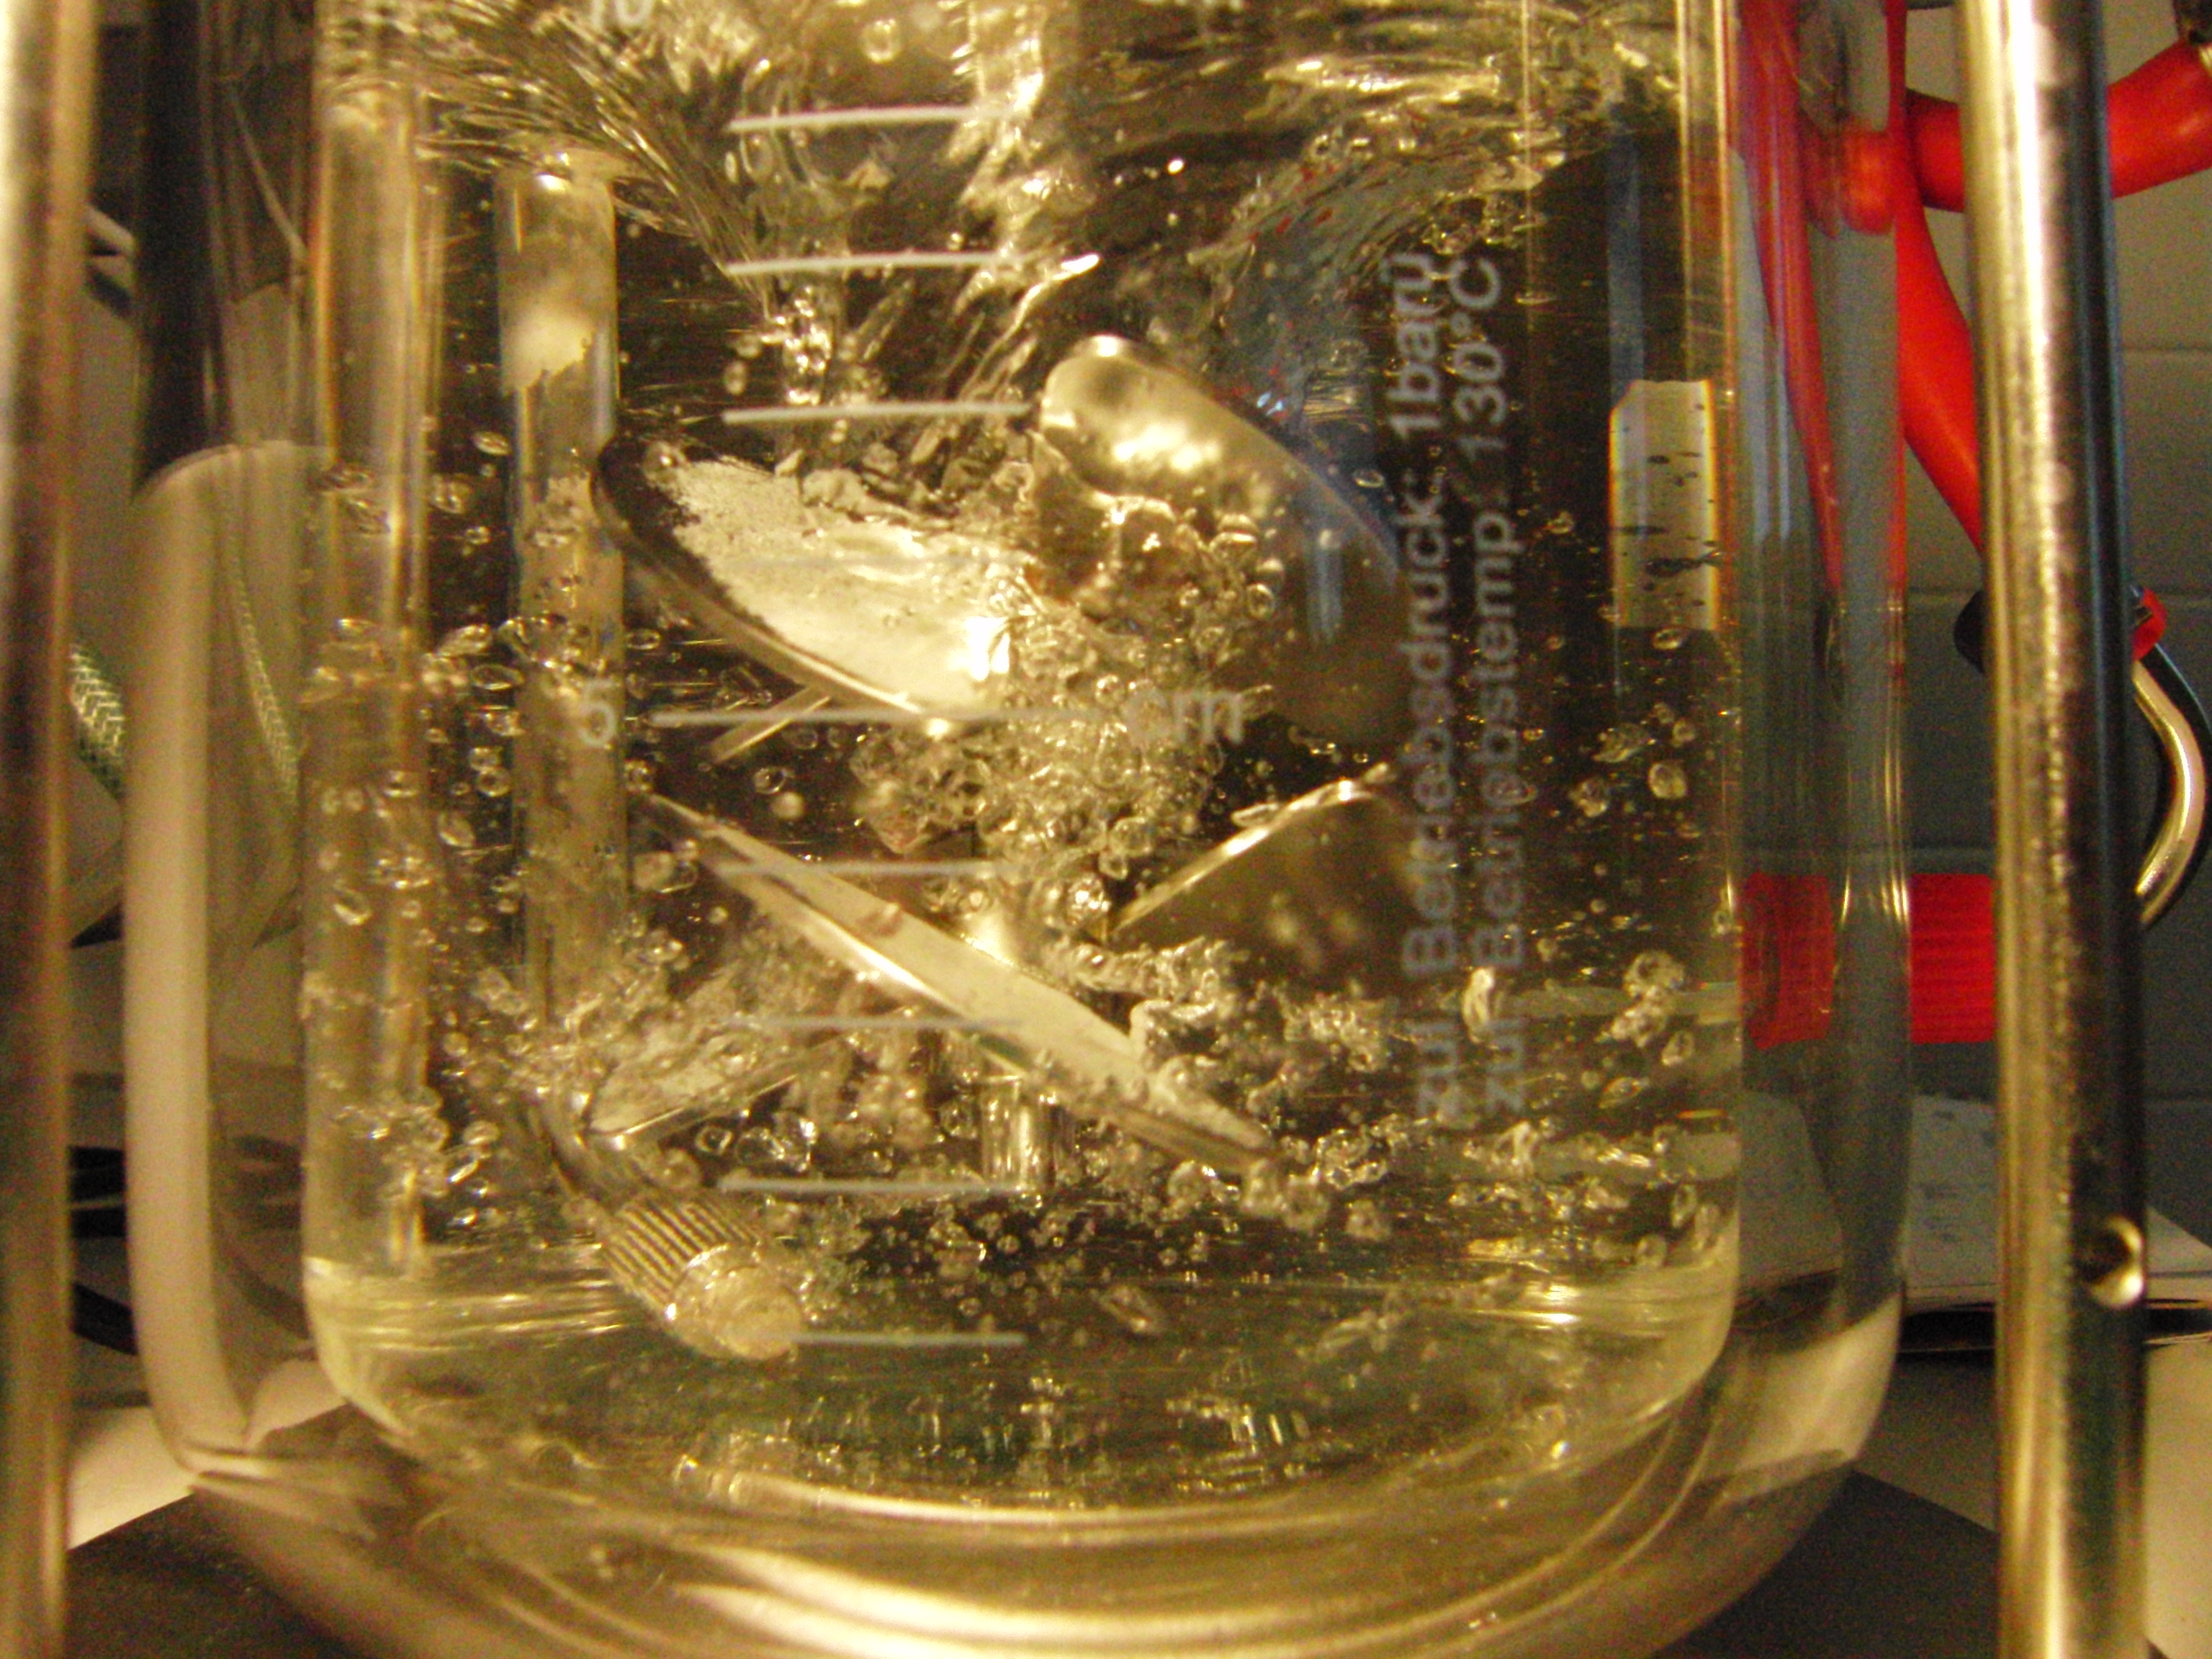
\includegraphics[height=4cm]{Blasenmessung/Versuch_1_4.JPG}}\label{blasengroesse4}
	\hspace{1cm}
	\subfigure[Bild 5]{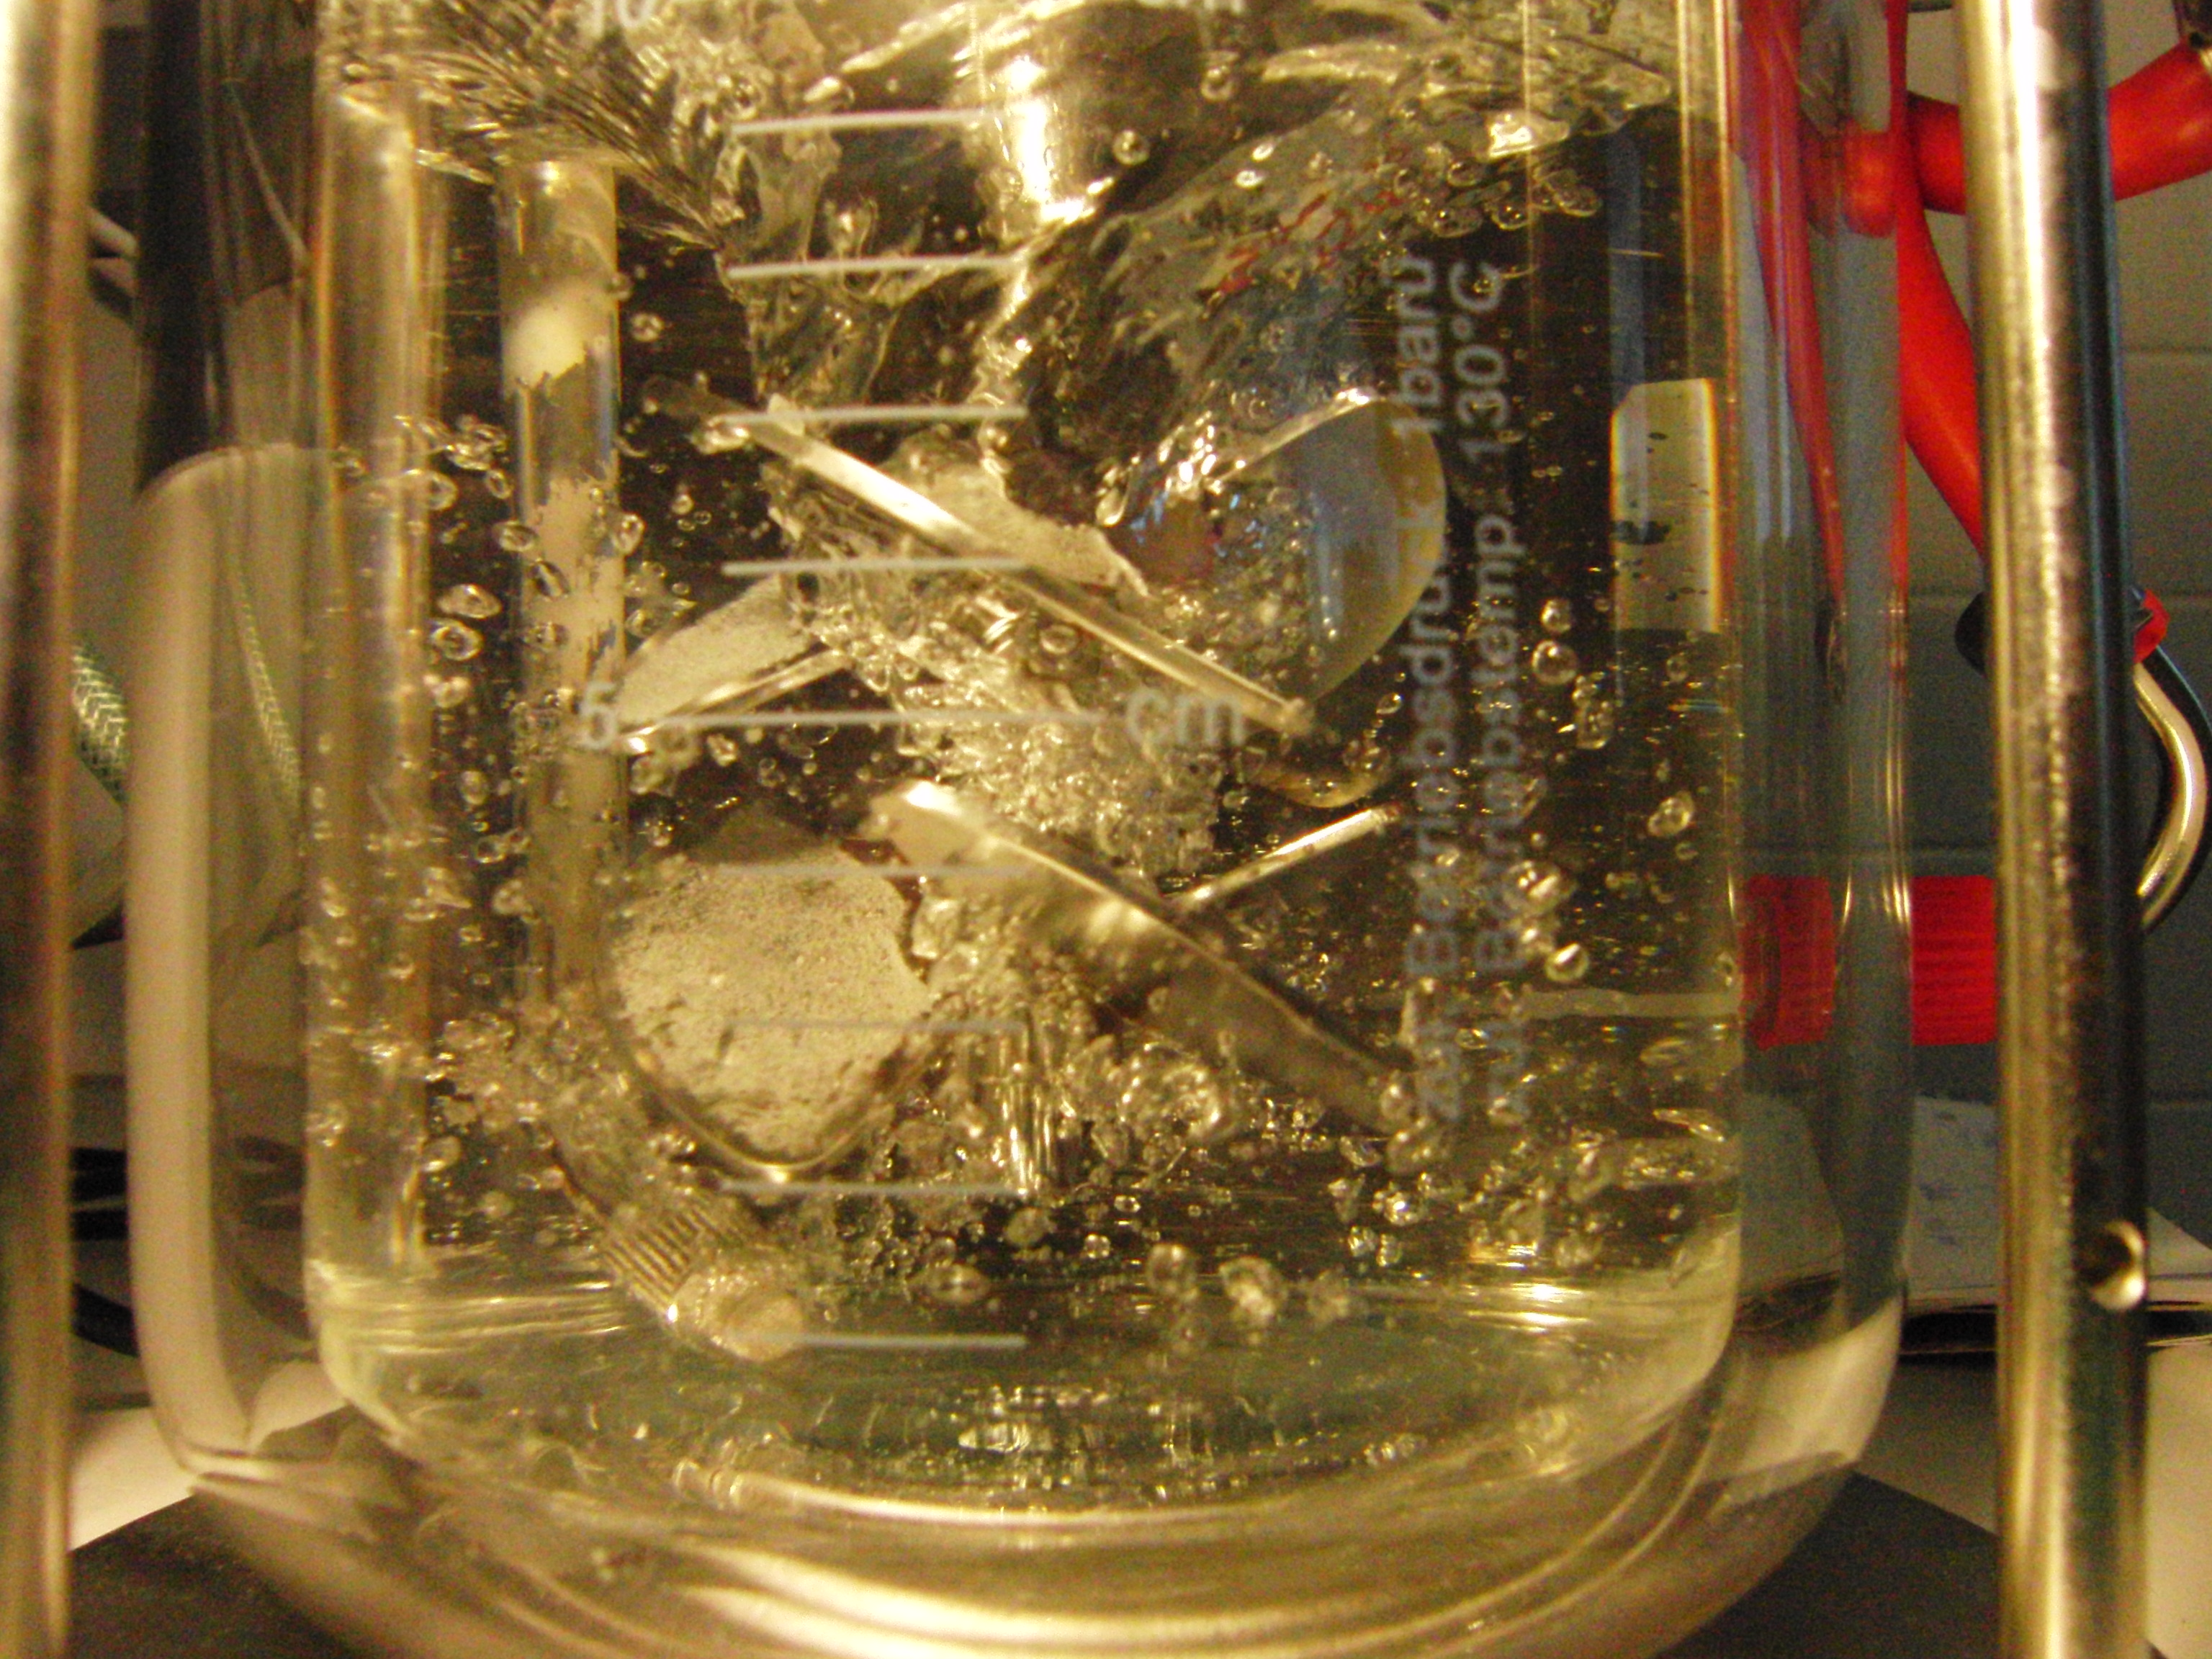
\includegraphics[height=4cm]{Blasenmessung/Versuch_1_5.JPG}}\label{blasengroesse5}
	\hspace{1cm}
	\subfigure[Bild 6]{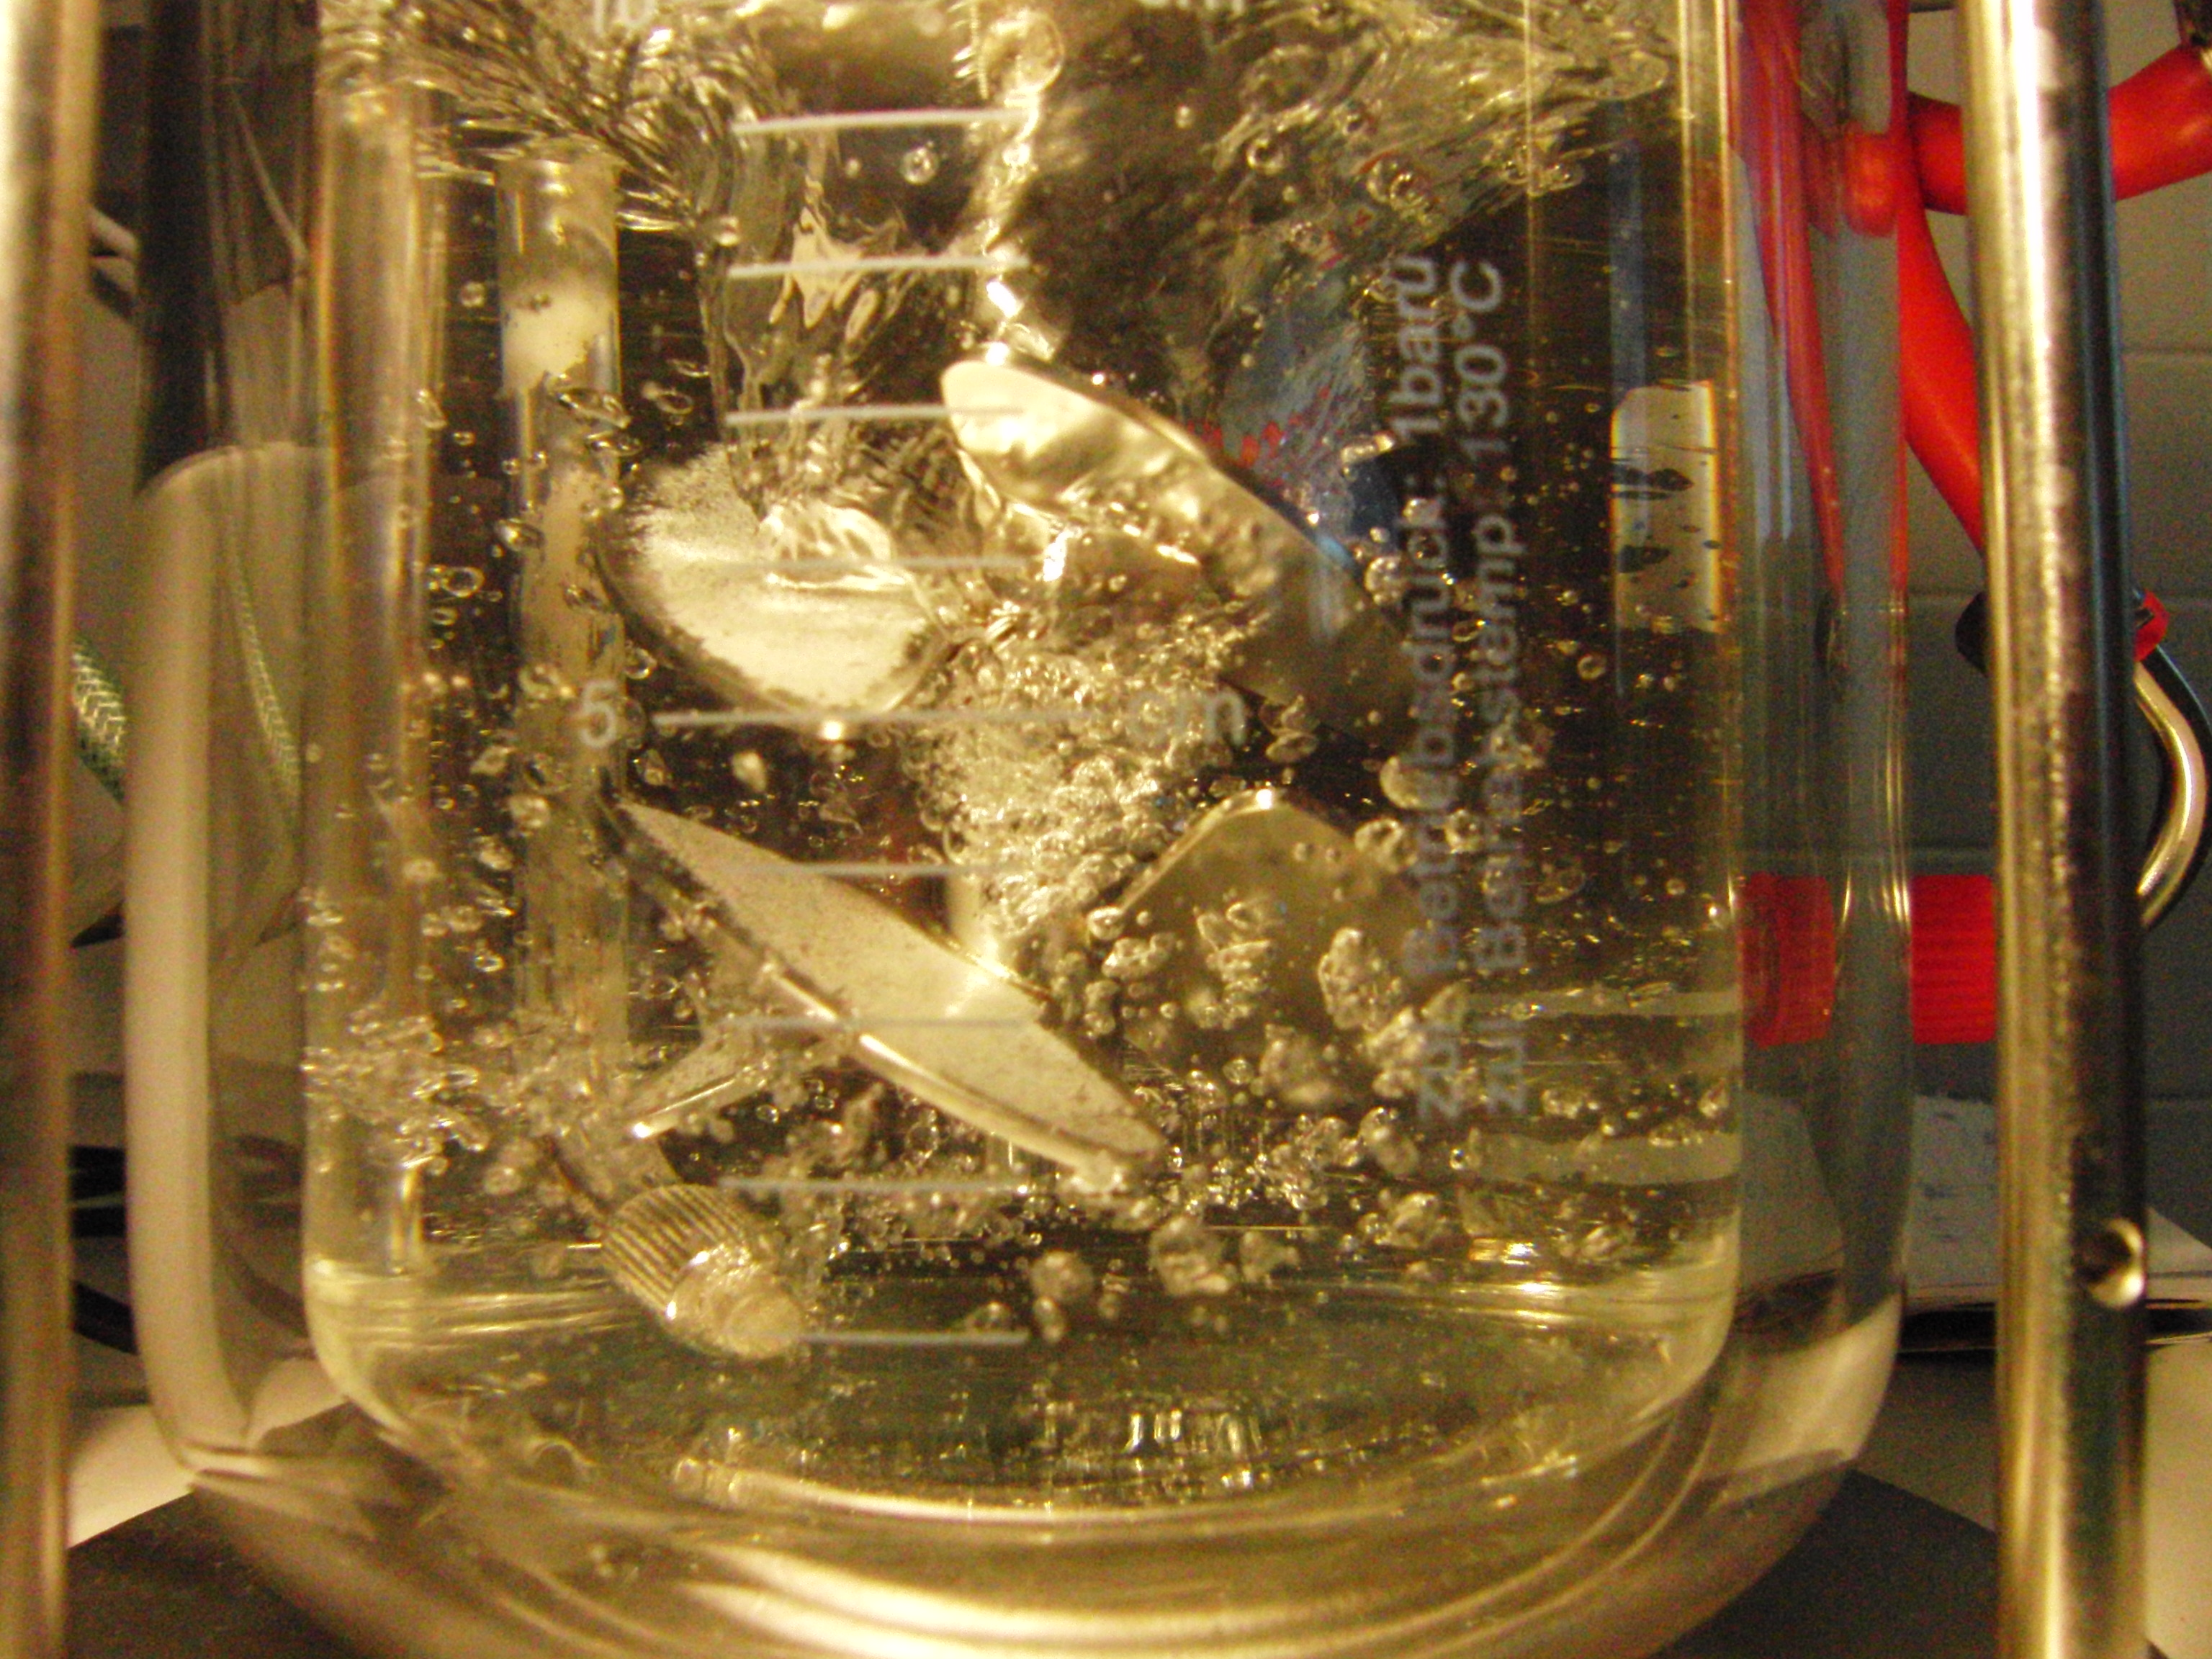
\includegraphics[height=4cm]{Blasenmessung/Versuch_1_6.JPG}}\label{blasengroesse6}
	\caption{Analyse der Blasengröße für Versuch Nr. 1}
	\label{Fotoserie1}
\end{center}	
\end{figure}
\noindent
Nach dieser Vorgehensweise kann die Blasenanzahl in den Fotoserien abgeschätzt werden. Die in Abbilung \ref{fig:Messung} dargestellten Quadranten werden auf jedes Bild gelegt. Anschließend werden die Blasen des rechten unteren Quadranten, genauer noch der vier abgetrennten Bereiche, gezählt und auf das ganze Reaktorvolumen hochgerechnet. Die teilende Linie in der Mitte wird immer zwischen den einzelnen Propellern des Rühres gezogen um annähernd auf die gleiche Blasenanzahl pro Quadrant zu kommen. Diese Auswahl stützt sich auf folgende Begründungen: 

\begin{itemize}
    \item Im linken unteren Eck befindet sich die Begasung und ist deshalb für die Zählung  nicht geeignet
    \item In der oberen Hälfte ist die deutliche Trombenbildung zu sehen, diese Turbulenzen machen es schwer in diesen Quadranten alle Gasblasen abzuschätzen.
    \item Die Trennline teilt die Hälften nicht im gleichen Flächenverhältnis. Durch die Trombe jedoch erlangt man ungefährt die gleiche Fläche/Volumen
    \item Im rechten unteren Quadranten sind die Gasblasen in den meisten Bildern einfach am besten zu erkennen
\end{itemize}

Somit ergeben sich folgende Werte für die mittlere Anzahl und den Durchmesser bezogen auf den Versuch. Die Werte pro Bild sind im Anhang ersichtlich. Die Werte werden mittels \textit{\textit{Excel}} ermittelt:

\begin{table}[H]
	\centering
	\caption{Abgeschätzter Blasendurchmesser und -anzahl | Zusammenfassung der Ergebnisse}
	\begin{tabular}{ccc}
		\toprule
		Versuch \# & Mittelwert & Standardabweichung \\
		\midrule
		\multicolumn{3}{c}{Blasenanzahl im Reaktor}\\
		\midrule
		1&872&$\pm 58,9$\\
		2&268&$\pm 32,7$\\
		3&670&$\pm 34,5$\\
		\midrule
		\multicolumn{3}{c}{Blasendurchmesser im Reaktor in mm}\\
		\midrule
		1&2,0&$\pm 0,18$\\
		2&3,7&$\pm 0,33$\\
		3&1,3&$\pm 0,08$\\	 
		\bottomrule
	\end{tabular}
	\label{tab:Blasendurchmesser_Anzahl_Zusammenfassung}
\end{table}

Grundsätzlich lässt sich aus den Bildern in Abbildung \ref{Fotoserie1} erkennen, dass sich die Blasen nachdem sie aus der Fritte der Begasung austreten, nahe der Rührerachse befinden und dann verteilt werden. Es zeigt sich auch, dass sich dabei die Gasblasen hauptsächlich im mittleren und oberen Bereich des Reaktors befinden. Dies ist vor allem bei der Auszählung der Gasblasen im rechten unteren Sektor zu sehen. Im unteren Bereich des Quadranten sind immer am wenigsten Blasen zu erkennen. Zudem erschwerte sich das Auszählen bzw. das Abschätzen des Durchmessers aufgrund von kumulierten Blasen an der Rührerachse und in Rührerblattnähe. Nur aufgrund der gemachten Bilder lässt sich daher schließen, dass der Reaktor nicht ideal durchmischt wird. Weiters zeigt sich dies auch durch das Ausbilden einer Trombe, welche ein Indiz für eine relativ schlechte Vermischung darstellt.\newline

Überdies lässt sich bei verschiedenen Rührerdrehzahlen und Begasungsströme ein deutlicher Trend erkennen. Bei niederer Drehzahl ($300\,\text{min}^{-1}$) sind mit freiem Auge wesentlich weniger Gasblasen im Reaktor zu sehen als bei höheren Drehzahlen. Dabei sind diese, aufgrund der gleichen Gasmenge aus Versuch 1 und 2 im zweiten Versuch deutlich größer und besitzen auch eine größere Standardabweichung (siehe Tabelle \ref{tab:Blasendurchmesser_Anzahl_Zusammenfassung}). Dies suggeriert, dass die Gasblasen im zweiten Versuch eher kumulieren. Weiters ist zu sehen, dass sich bei hoher Drehzahl und niederem Gasstrom sich die Gasblasen besser verteilen lassen und daher auch einen geringeren Durchmesser besitzen. Die Anzahl erniedrigt sich nicht drastisch, ist jedoch im Durchschnitt kleiner als im ersten Versuch. Selbiges ist für den durchschnittlichen Durchmesser zu beobachten. Die Zählmethode und Abmessung der Blasen birgt einige Fehlerquellen. Der Einfluss dieser Methoden auf die tatsächlichen Werte soll im Kapitel 6 auf Seite \pageref{Interpretation} diskutiert werden. Abschließend kann mit den in diesem Abschnitt erhaltenen Werten die spezifische Oberfläche abgeschätzt werden. 

\subsection{Resultierende spezifische Oberfläche und $k_l$-Wert}

Die Berechnung wird exemplarisch für den ersten Versuch durchexerziert.\\
Zunächst wird die Oberfläche einer Blase berechnet.

\begin{gather}
    S_b = d_b^2\cdot \pi \\
    \notag\\
    S_b = \left(0,002\,\m\right)^2 \cdot \pi = 1,25664 \cdot 10^{-5}\,m^2\notag
\end{gather}

Nun wird die Oberfläche aller Blasen berechnet und auf das Volumen des Fluids im Reaktor bezogen.

\begin{gather}
    S_{ges} = n_b \cdot S_b\\
    \notag\\
    S_{ges} = 872 \cdot 1,25664 \cdot 10^{-5}\,m^2 = 0,01096\,\m^2\notag\\
    \notag\\
    \notag\\
    A_{spez} = \frac{S_{ges}}{V_R}\\
    \notag\\
    A_{spez} = \frac{0,01096\,\m^2}{0,00234\,\m^3} = 4,683\,\m^{-1}\notag
\end{gather}

Mit dem ermittelten $k_la$-Wert und der spezifischen Austauschfläche kann nun der $k_l$-Wert berechnet werden. Hierbei wird der $k_la$-Wert vom Austreiben und Aufsättigen gemittelt.

\begin{gather}
    k_l = \frac{k_La}{A_{spez}}\\
    \notag\\
    k_l = \frac{0,003704\,\s^{-1}}{4,683\,\m^{-1}} = 0,000791\,\frac{\m}{\s}
\end{gather}

Die berechneten $k_l$-Werte und Zwischengrößen sind in Tabelle \ref{tab:kl} aufgelistet.


% Table generated by \textit{Excel}2LaTeX from sheet 'kl'
\begin{table}[htbp]
  \centering
  \caption{Ergebnisse $k_l$-Werte}
    \begin{tabular}{ccccccccc}
    \toprule
    Versuch & $S_b$ / m$^2$ & $S_{ges}$ / m$^2$ & $V_R$ / m$^3$ & $A_{spez}$ / m$^{-1}$ & $k_la$ / s$^{-1}$   & $k_l$ / m\,s$^{-1}$\\
    \midrule
    1      & 1,25664E-05 & 0,01095788 & \multirow{3}[0]{*}{0,00234} & 4,683 & 0,003704 & 0,000791 \\
    2     &  4,30084E-05 & 0,01152625 &       & 4,926 & 0,002710 & 0,000550 \\
    3      & 5,30929E-06 & 0,00355723 &       & 1,520 & 0,003197 & 0,002103 \\
    \bottomrule
    \end{tabular}%
  \label{tab:kl}%
\end{table}%

In Tabelle \ref{tab:kl} zeigt sich, dass trotz der kleinsten durchschnittlichen Blasengröße und der resultierenden kleinen Oberfläche der $k_l$-Wert fast doppelt so groß ist wie im ersten Versuch. Die annähernd gleich große Anzahl spielt dabei nur eine untergeordnete Rolle, da der Durchmesser mit der dritten Potenz in die Gleichung eingeht. 
%Interpretation: wegen Fehlerquellen nur wenig aussagekräftig, Literaturrecherche wäre zu aufwendig und wird daher nicht weiter durchgeführt.


\section{Dimensionslose Kennzahlen der Versuchsreihen}

\subsection{Berechnung der Kennzahlen}
\label{cap:Ber_Kenz}
Zur Beschreibung der Strömung im Rührkessel werden die quadrierte Froude-Zahl $Fr'$, die Reynolds-Zahl der Rührerströmung $Re_{SR}$ und die Gas Flow Number $Fl$ berechnet. Die Stoffdaten für die vorherrschenden Drücke und Temperaturen wurden mit dem thermodynamischen Berechnungstool von Berndt Wischnewski ermittelt \cite{Peacesofware}, der Gasfluss und die Rührerdrehzahl sind in Kapitel \ref{sec:versuchsdurchfuehrung} bereits aufgelistet und der Rührerdurchmesser ist in Abbildung \ref{fig:masseReactor} ersichtlich. Die Berechnungen werden Beispielsweise für das Aufsättigen beim ersten Versuch durchexerziert:

\begin{gather}
    Re_{SR} = \frac{\rho \cdot N \cdot D^2}{\mu} \\
    \notag\\
    Re_{SR} = \frac{997,71\,\frac{\text{kg}}{\text{m}^3} \cdot 7,5\,\frac{1}{\s} \cdot \left(0,06\,\m \right)^2}{9,43\cdot 10^{-4}\,\text{Pa\,s}} =  28541,54\notag\\
    \notag\\
    \notag\\
    Fr' = \frac{D \cdot N^2}{g} \\
    \notag\\
    Fr' = \frac{0,06\,\m \cdot \left(7,5\,\frac{1}{\s}\right)^2}{9,81\,\frac{\m}{\s^2}} = 0,34403\notag\\
    \notag\\
    \notag\\
    Fl'_{aufsättigen} = \frac{\dot{G}}{N \cdot D^3}\\
    \notag\\
    Fl'_{aufsättigen} = \frac{9,166\,\frac{\text{l}}{\text{h}}}{1000\,\frac{\text{l}}{\m^3} \cdot 3600\,\frac{\s}{\h} \cdot 7,5\,\frac{1}{\text{s}} \cdot \left(0,06\,\m\right)^3} = 0,00157\notag
\end{gather}

Da sich der Gasfluss beim Austreiben mit Stickstoff von dem der Luft beim Aufsättigen unterscheidet, wird eine zweite Gas Flow Number berechnen:

\begin{gather*}
    Fl'_{austreiben} = \frac{9,324\,\frac{\text{l}}{\text{h}}}{1000\,\frac{\text{l}}{\m^3} \cdot 3600\,\frac{\s}{\h} \cdot 7,5\,\frac{1}{\text{s}} \cdot \left(0,06\,\m\right)^3} = 0,00160\notag
\end{gather*}

Die Kennzahlen für alle Versuche sind in Tabelle \ref{tab:kennzahlen} aufgelistet. Es ist dabei erkennbar, dass hinsichtlich der Strömungsverhältnisse in einem Bereich von $Re$ ca. 20.000-30.000 gearbeitet wird und aufgrund der geringen $Fr'$-Zahlen der Einfluss der Schwerkraft weniger signifikant ist. 

% Table generated by \textit{Excel}2LaTeX from sheet 'korrelation'
\begin{table}[H]
  \centering
  \caption{Berechnete Kennzahlen für die verschiedenen Betriebspunkte}
    \begin{tabular}{ccccc}
    \toprule
    Versuch & Vorgang & $Re$    & $Fl$    & $Fr'$ \\
    \midrule
    \multirow{2}[0]{*}{1} & austreiben & 28541,54 & 0,000825 & 0,3440 \\
          & aufsättigen & 28541,54 & 0,000839 & 0,3440 \\
          \midrule
    \multirow{2}[0]{*}{2} & austreiben & 19680,93 & 0,002290 & 0,1529 \\
          & aufsättigen & 19680,93 & 0,002330 & 0,1529 \\
          \midrule
    \multirow{2}[0]{*}{3} & austreiben & 29859,63 & 0,001572 & 0,3440 \\
          & aufsättigen & 29859,63 & 0,001599 & 0,3440 \\
          \bottomrule
    \end{tabular}%
  \label{tab:kennzahlen}%
\end{table}%


\subsection{Korrelation zur Bestimmung des $k_la$-Wertes}
\label{cap:Korrelation}
Mittels der Statistik-Software $R$ wird eine Korrelation zwischen den dimensionslosen Kennzahlen und dem $k_la$-Wert berechnet.

\begin{equation}
    k_La = Re_{SR}^{-0,6235} \cdot \left(Fr'\right)^{-0,1792} \cdot Fl^{\,0,4441}
\end{equation}

Nach dem Berechnungsmodell aus \cite{wilkinson1973symbolic} beträgt der sogenannte \glqq residual standard error\grqq\;0,000822 bei drei Freiheitsgraden und sechs Beobachtungen. Dabei handelt es sich um die Wurzel der Residuenquadratsumme geteilt durch $n - k$, wobei $n$ die Anzahl der Beobachtungen und $k$ die Anzahl der Regressoren ist.\\
\\
Mit dieser Korrelation können nun Modellwerte mit den Kennzahlen der Messwerte berechnet werden und damit das $R^2$ des Modells bestimmt werden (analog zu Kapitel \ref{sec:kla}). Das $R^2$ des Modells beträgt 0,326. In Tabelle \ref{tab:korrelation} sind die Modellwerte und die gemessenen Werte gegenübergestellt.

% Table generated by \textit{Excel}2LaTeX from sheet 'korrelation'
\begin{table}[H]
  \centering
  \caption{Gemessene und aus der Korrelation berechnete $k_la$-Werte}
    \begin{tabular}{ccccccc}
    \toprule
    Versuch & Vorgang & $Re_{SR}$    & $Fl'$    & $Fr$    & $k_la$ in $\frac{1}{\text{s}}$   & $k_La_{Modell}$ \\
    \midrule
    \multirow{2}[0]{*}{1} & austreiben & 28541,54 & 0,000825 & 0,3440 & 0,003056 & 0,003705 \\
          & aufsättigen & 28541,54 & 0,000839 & 0,3440 & 0,004353 & 0,003694 \\
          \midrule
    \multirow{2}[0]{*}{2} & austreiben & 19680,93 & 0,002290 & 0,1529 & 0,002312 & 0,002714 \\
          & aufsättigen & 19680,93 & 0,002330 & 0,1529 & 0,003107 & 0,002705 \\
          \midrule
    \multirow{2}[0]{*}{3} & austreiben & 29859,63 & 0,001572 & 0,3440 & 0,003853 & 0,003209 \\
          & aufsättigen & 29859,63 & 0,001599 & 0,3440 & 0,002541 & 0,003199 \\
          \bottomrule
    \end{tabular}%
  \label{tab:korrelation}%
\end{table}%

Das Modell liefert gute Ergebnisse, die vorhergesagten Werte entsprechen dem Mittelwert des $k_la$-Wertes aus Aufsättigen und Austreiben.\\
\\
Da die verschiedenen Vorgänge für die Versuche den gleichen Betriebspunkt darstellen und die kleine Abweichung von $Fl'$ durch den geringen Dichteunterschied bei der Verwendung von Stickstoff und Luft zustande kommt, erscheint es sinnvoll die Vorgänge der einzelnen Versuche zusammenzufassen und zu mitteln. Somit bleiben nur mehr drei Beobachtungen übrig. Da nun die Anzahl an Modellvariablen gleich der Anzahl an Beobachtungen ist, wird $R^2$ = 1. Nun muss eine Variable aus der Korrelation ausgeschlossen werden. Werden die Kennzahlen übereinander dargestellt ergibt sich:

\begin{figure}[H]
    \centering
    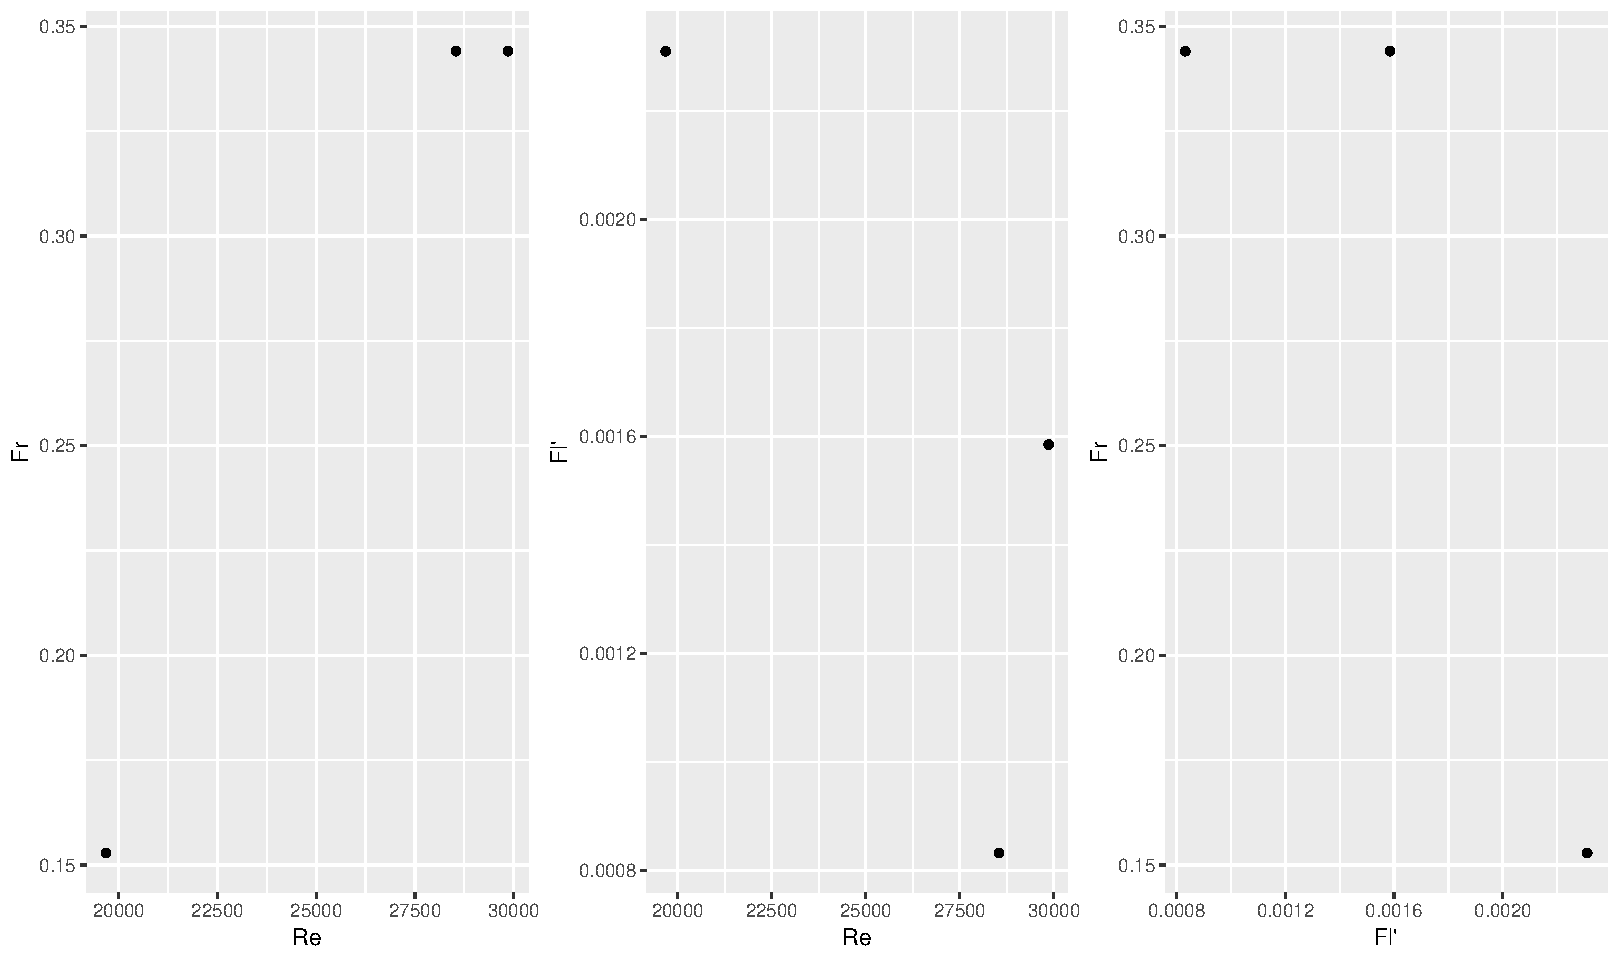
\includegraphics[width=1\textwidth]{Graphics/kennzahlen.pdf}
    \caption[Darstellung]{Darstellung aller Kombinationen der Kennzahlen}
    \label{fig:kennzahlen}
\end{figure}

In Abbildung \ref{fig:kennzahlen} ist ersichtlich, dass bei der Verwendung von $Re$ und $Fl'$ die Kennzahlen nie den gleichen Wert zweimal annehmen, daher werden diese Kennzahlen für die neue Korrelation verwendet. Somit lautet die neue Gleichung:

\begin{equation}
    k_La = Re_{SR}^{-0,8920} \cdot \left(Fl'\right)^{-0,5033}
\end{equation}

Der residual standard error für diese Korrelation beträgt $0,0007252$ bei einem Freiheitsgrad.

% Table generated by \textit{Excel}2LaTeX from sheet 'korrelation (2)'
\begin{table}[H]
  \centering
  \caption{Gemessene und aus der Korrelation berechnete $k_la$-Werte | zwei Parameter}
    \begin{tabular}{ccccc}
    \toprule
    Verusch & $Re_{SR}$    & $Fl'$    & $k_la$   & $k_La_{Modell}$ \\
    \midrule
    1     & 28541,54 & 0,000832 & 0,003704 & 0,003765 \\
    2     & 19680,93 & 0,002310 & 0,002710 & 0,003137 \\
    3     & 29859,63 & 0,001585 & 0,003197 & 0,002615 \\
    \bottomrule
    \end{tabular}%
  \label{tab:korrelation-2param}%
\end{table}%

Zu erwähnen gilt, dass die Werte der Korrelation mit zwei Parameter etwas ungenauer sind und stärker von den gemessenen Werten abweichen. Bei der Auswahl der Modellgleichung wurde das Skriptum zur Laborübung \cite{Labor_Skript} zu Rate gezogen. Dort sind einige Korrelationen für den $k_la$-Wert aufgelistet, und jede dieser Korrelationen ist ein Modell mit nur einem Term.\\
\\
Als drittes Modell wird eine lineare Regression mit zwei Variablen vorgeschlagen:

\begin{equation}
    k_La = 1,150 \cdot 10^{-7} \cdot Re_{SR} + 0,1174 \cdot Fl'
\end{equation}

Das $R^2$ des Modells beträgt $0,9899$.

% Table generated by \textit{Excel}2LaTeX from sheet 'korrelation (2)'
\begin{table}[H]
  \centering
  \caption{Gemessene und aus der Korrelation berechnete $k_la$-Werte | linear}
    \begin{tabular}{ccccc}
    \toprule
    Versuch & $Re_{SR}$ & $Fl'$ & $k_la$ & $k_La_{Modell}$ \\
    \midrule
    1     & 28541,54 & 0,000832 & 0,003704 & 0,003380 \\
    2     & 19680,93 & 0,002310 & 0,002710 & 0,002535 \\
    3     & 29859,63 & 0,001585 & 0,003197 & 0,003620 \\
    \bottomrule
    \end{tabular}%
  \label{tab:korrelation-lin}%
\end{table}%

Bei Regressionen mit einem Regressor liegt der Gültigkeitsbereich zwischen dem kleinsten und größten Wert dieses Regressors. Bei mehreren Regressoren lässt sich der Gültigkeitsbereich am einfachsten graphisch darstellen.

\begin{figure}[H]
    \centering
    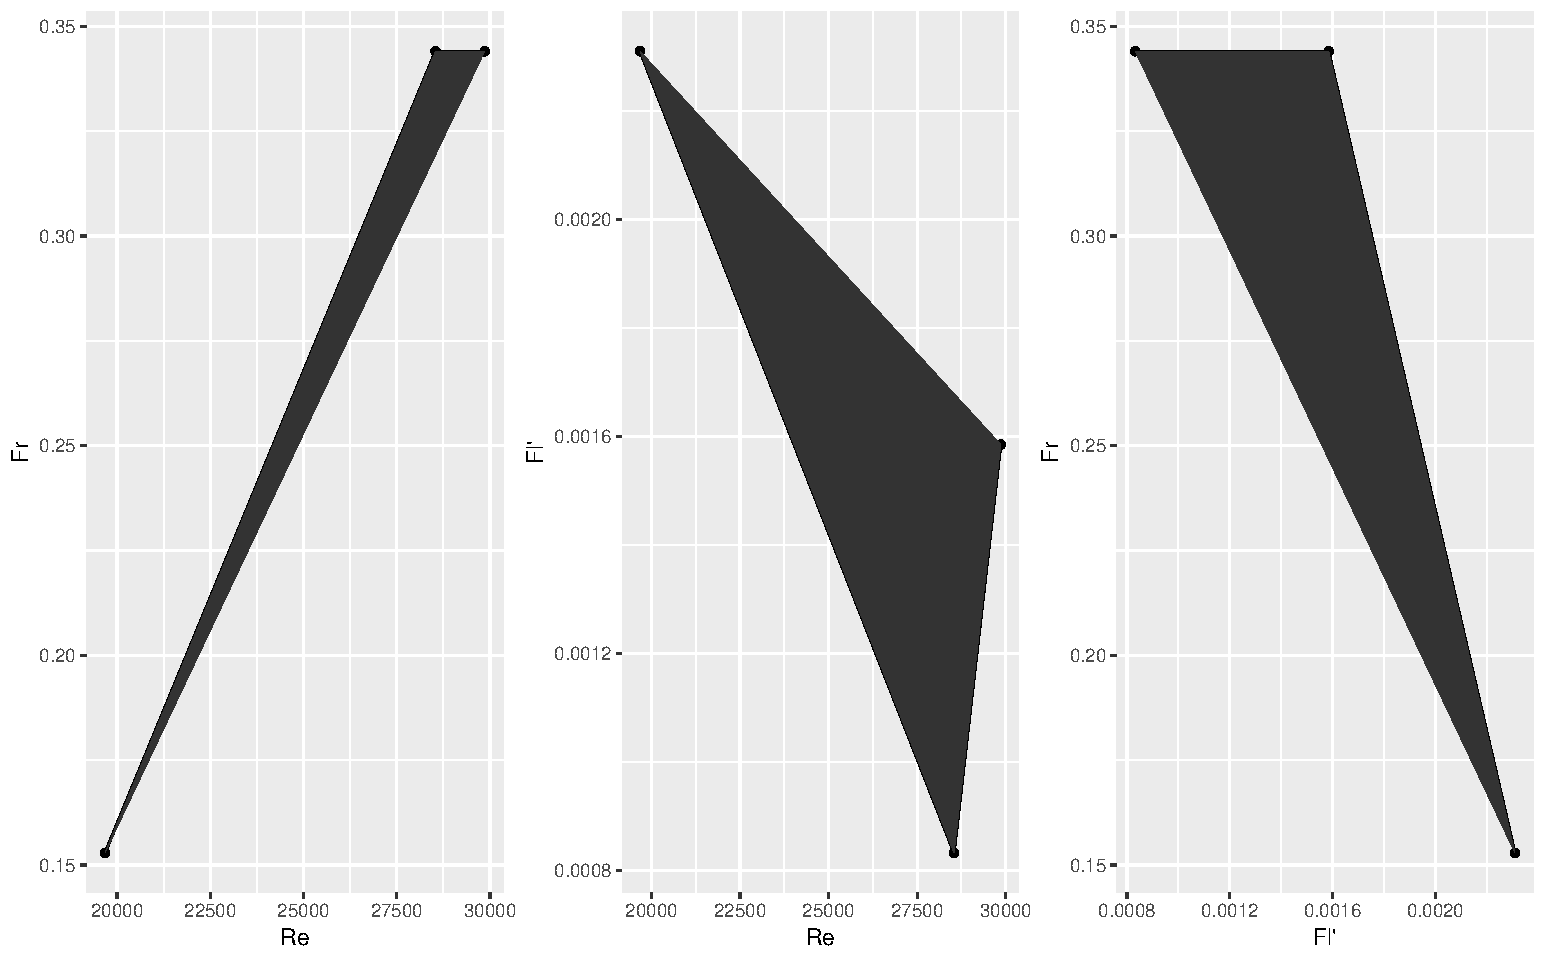
\includegraphics[width=1\textwidth]{Graphics/gueltigkeit.pdf}
    \caption[Gültigkeitsbereiche]{graphische Darstellung der Gültigkeitsbereiche}
    \label{fig:gueltigkeit}
\end{figure}

Für die beiden zwei-Parameter-Modelle muss der Punkt welcher dem Modell übergeben wird innerhalb der Fläche des mittleren Diagramms liegen. Für die erste Korrelation mit allen drei Kennzahlen muss der Punkt in allen drei Flächen liegen.



\chapter{Interpretation}

Aufgrund der erhaltenen Ergebnisse können nun diese Daten, Werte und Korrelationen interpretiert und deren physikalische Bedeutung bzw. die Einflüsse auf die Ergebnisse argumentiert werden.

\section{$k_l$-\text{Wert} Abschätzung}
\label{Interpretation}Durch die gewählten Methoden bei der Auszählung der Blasen und der Abschätzung des Blasendurchmessers ergeben sich diverse Fehlerquellen. Die Charakterisitka dieser und die Auswirkungen auf die Ergebnisse sollen in folgendem Abschnitt erläutert werden. Als erstes fällt bei genauerer Betrachtung auf, dass sich auf den Bildern, trotz hoher Qualität, nicht immer alle Blasen erkenn lassen. Zum Teil sind es oft verschwommene blasenähnliche Konstrukte, bei denen es nicht ganz sicher ist, ob es nicht mehrere oder gar keine Blasen sind. Des Weiteren zeigen sich in manchen Abbildungen Spiegelungen, welche ebenfalls als Blasen interpretiert werden können, man sich aber nicht sicher sein kann. Grundsätzlich wurde vereinbart, dass Blasen bei denen es nicht sicher war, ob es denn solche sind, nicht gezählt werden. Vor allem in Versuch 1 und 3 wurden manche Blasen nicht erkannt, bzw. waren nicht eindeutig als Blasen zu identifizieren, da auch die Größe der Blasen und die Bildqualität dazu beitrugen. Dies verfälscht natürlich die absolute Anzahl der Blasen, vor allem wenn der Sektor mit vier multipliziert wird. So vernachlässigt man zum Beispiel die Oberfläche von 40 Blasen, wenn im rechten unteren Quadranten 10 Blasen nicht zu $100\,\%$ zu erkennen sind. Weiters sind die Bilder nur eine Aufnahme von vorne. Das bedeutet, dass Blasen, welche hinter der Rührerachse oder dem Blatt befinden nicht bei der Zählung oder der Durchmesser Messung berücksichtigt werden können. Darüber hinaus werden Blasen vernachlässigt, welche sich hinter einer großen Blasenanhäufungen befinden. Die Blasenanhäufung oder kumulierte Blasen sind ebenfalls nicht eindeutig einer genauen Blasenanzahl zuzuordnen. Oft wurde \glqq geraten\grqq\, um eine ungefähre Anzahl in solcher einer Anhäufung zu bestimmen. Dabei wurde vor allem auf optische Aspekte, wie die Suche nach Rundungen in der Anhäufung geachtet. Bei der Abschätzung des Durchmessers wurde mit den Blasenanhäufungen sehr vorsichtig umgegangen. Diese wurden bei nicht eindeutiger Zuordnung oder ganz außen vor gelassen um keine wesentliche Abweichung des mittleren Durchmessers zu erlangen. Dieser würde dadurch sehr wahrscheinlich viel zu hoch eingeschätzt werden (10 - 15\,mm statt 2\,mm bei großen Anhäufungen), was die ganze Messung verfälschen würde. Zudem gibt es bei der Abschätzung des Blasendurchmesser noch weitere Fehlerquellen. Zum einen ist die Form solch einer Blase im Reaktor nicht immer kreis- bzw. kugelförmig. Daher gilt es zu evaluieren welcher Durchmesser von zum Beispiel einem Ellipsoid gewählt wird. Es wurde deshalb ein Mittelwert der Durchmesser gewählt um sich einer äquivalenten Kugel anzunähern. Zum anderen ist die Methode der zufälligen Wahl mancher Blasen nicht die genaueste. Der Aufwand wäre aber zu hoch alle Blasen oder Blasen eines Sektors abzumessen. Es wurde versucht ein guter Kompromiss zwischen der Abmessung kleinen und großen Blasen zu finden, da zum Beispiel sehr kleine Blasen ($<0.5\,mm$) große Auswirkunken auf die Spezifische Oberfläche und den Stoffaustausch im Reaktor haben.\newline

Ergänzend lässt sich über die Blasenanzahl und den Blasendurchmesser aus Tabelle \ref{tab:Blasendurchmesser_Anzahl_Zusammenfassung} sagen, dass diese plausible Dimensionen annehmen und die beschrieben Korrelationen schlüssig sind. Durch die niedere Drehzahl zum Beispiel, lässt sich der Gasstrom weniger gut verteilen und es entstehen größere Blasen. Durch die gleiche eingebrachte Gasmenge, wie zum Beispiel im Versuch 1, und das Volumen ja pro Stunde gleich bleibt, sind weniger Blasen im Reaktor anzutreffen. Selbiges gilt für die Unterscheidung vom ersten und dritten Versuch. Auch diese Versuche zeigen rein mechanisch erwartete Werte für die Blasenanzahl und den Blasendurchmesser in Relation zu einander. Durch die hohe Drehzahl im dritten Versuch werden die Gasblasen gut zerteilt. Da aber nun weniger Volumen pro Stunde in den Reaktor gelangt, tut sich der Rührer leichter dieses zu zerteilen. Es entstehen kleinere Blasen. Zusätzlich sind es weniger, da die Gasmenge geringer ist. Bei ganzheitlicher Betrachtung zeigt sich optisch, dass die Rührerdrehzahl mehr Einfluss ausübt, als der Gasvolumenstrom. Der Einfluss auf die Konzentration bzw. den Stoffaustausch ($k_La-\text{Wert}$) mit Einfluss der Fehlerquellen ist in diesem Kapitel folglich noch ersichtlich.\newline

In Tabelle \ref{tab:kl} ist ersichtlich, dass die spezifische Austauschfläche bei Versuch 1 und 2 annähernd gleich ist. Da die $k_la$-Werte in der gleichen Größenordnung liegen, sind auch die Stoffdurchgangskoeffizienten ähnlich.\\
Bei Versuch 3 ist die spezifische Austauschfläche kleiner, da aber auch hier der $k_la$-Wert im gleichen Wertebereich wie für die anderen Versuche liegt, ist der Stoffdurchgangskoeffizient um den Faktor 10 größer. Der höhere Stoffdurchgangskoeffizient bei niedrigerer Austauschfläche aber vergleichbarem $k_la$-Wert suggeriert dass bei diesem Vergleich eine andere Stoffübergangszahl vorherrscht.  Laut Seader et al. \cite{seader1998separation} setzt sich die Stoffübergangszahl wie folgt zusammen:

\begin{equation}
    \beta = \frac{\dot{n}_A}{A \cdot \Delta c_A}
\end{equation}

Und der Zusammenhang zwischen Stoffdurchgangskoeffizient und Stoffübergangszahl:

\begin{equation}
    \frac{1}{k_l} = \frac{1}{\beta_l} + \frac{1}{H_{12} \cdot \beta_g}
\end{equation}

Das Konzentrationsgefälle unterscheidet sich zwischen den Versuchen nicht merklich. Der Stoffmengenstrom $\dot{n}_A$ ist beim letzten Versuch durch den reduzierten Gasstrom geringer. Ebenso ist die Austauschfläche $A$ durch den kleineren Blasendurchmesser geringer. Die kleinere Austauschfläche fällt stärker ins Gewicht als der reduzierte Gasstrom, was zu einer höheren Stoffübergangszahl und somit zu einem höheren Stoffdurchgangskoeffizient führt. 

\section{Konzentrationsverlauf und $k_la$ - \text{Wert}}

Hinsichtlich der Konzentrationsverläufe in Abbildung \ref{fig:c_aus_versuch1} ff. lässt sich im Allgemeinen feststellen, dass ein exakter Nullwert in der flüssigen Phase nicht erreicht wird und dieser mit 2\,mg$\cdot$l definiert auch bei allen Versuchen als erreichbar angesehen werden kann. Selbiges gilt für die vorberechnete Sättigungskonzentration mit ca. 7\,mg$\cdot$l, welche beim ersten Versuch mit höchster Drehzahl und Gasdurchfluss erreicht wird, bei Versuch 2 und 3 jedoch nicht. Folglich lässt sich bei Betrachten des Maximums von Versuch 2 und 3 feststellen, dass aufgrund des größeren Maximums bei Versuch 3 der Einfluss der Rührerdrehzahl auf die einbringbare Sauerstoffmenge größer ist als der Einfluss des Gasdurchflusses. Dies lässt auch den Schluss zu, dass die aussagekräftigste dimensionslose Kennzahl zur Beschreibung des Vorganges die Reynolds-Zahl mit der Umfangsgeschwindigkeit des Rührers ist. Bezugnehmend auf die aus den Konzentrationsverläufen ermittelten $k_la$-Werte ist die signifikanteste Aussage, dass eine Differenz zwischen den Vorgängen Austreiben und Aufsättigen vorhanden ist, obwohl die Versuchsparameter konstant gehalten werden. Der Einfluss der Gasphase, welche den Lösungsvorgang bzw. den Austreibungsvorgang hervorrufen soll, ist also nicht zu vernachlässigen, da mit Stickstoff beispielsweise bei Versuch 1 und 2 höhere $k_la$-Werte erhalten werden. Eine physikalische Grundlage bzw. ein Muster für diese Differenz kann aufgrund der geringen Anzahl an gefahrenen Betriebspunkten nicht identifiziert werden.
\\
\\
Bei Betrachtung der Konzentrationsverläufe und $k_la$-Werte können Fehlerquellen bzw. Ursachen für die Abweichungen und Differenzen erkannt werden. Diese liegen einerseits in der Tatsache, dass im untersten Teil des flüssigen Reaktorvolumens am wenigsten Luftblasen sichtbar sind (siehe Abbildung \ref{Fotoserie1}) und daher am Ort der Probenahme die Konzentration an gelöstem $\ch{O2}$ geringer gemessen wird als tatsächlich im gesamten Volumen vorhanden. Zudem ist ein Totvolumen innerhalb der Schläuche vorhanden, welches an den in Probenahme- und Rückführschläuchen vorhandenen Luftblasen erkennbar ist. Das Totvolumen beeinträchtigt den Durchfluss der zu messenden Flüssigkeit und außerdem die Konzentration des gelösten Sauerstoffs. Zudem werden Gasblasen aus der Fritte in der Flüssigkeit durch den Rührer dispergiert und steigen durch den Dichteunterschied an die Oberfläche, wobei eine Zerteilung der Blasen nicht immer sofort möglich ist und daher diese einfach aufsteigen und bei einem geringen Oberfläche zu Volumen Verhältnis einen kleineren Stoffübergang aufweisen. Somit gehen geringere Stoffmengen in die flüssige Phase über. Ein weiterer Einflussfaktor, ist die durch den Rührer verursachte Trombe, welche das Messen des Hold-Up durch den Anstieg des Flüssigkeitsspiegels unmöglich macht. Die Trombe erzeugt außerdem Wirbel durch welche die Gasblasen schlechter vermischt werden und bei Ankunft am oberen der beiden Rührer in die Trombe eingearbeitet werden. Dadurch werden sie an der Welle agglomeriert oder im Wirbel mehrfach von oben nach unten transportiert. Sprich, sie können für den Stoffübergang nicht effektiv genutzt werden.\newline

An dieser Stelle sei noch angemerkt, dass $R^2$ sich laut Spiess et al. \cite{rquadrat} nur schlecht zur Beschreibung von nicht-linearen Modellen eignet. Die Vorgehensweise zur Berechnung des $k_la$-Wertes durch Maximierung von $R^2$ ist sinnvoll und zielführend, jedoch sollte bei der Evaluierung des Modells oder dem Vergleich mit anderen Modellen besser auf andere Kriterien zurückgegriffen werden.

\section{Dimensionslose Kennzahlen und Korrelation zur Bestimmung des $k_La - \text{Wertes}$}

\label{Bestimmung_Strömung}Über die beiden dimensionslosen Kennzahlen $Fr'\;\&\; Fl$ lässt sich ein bestimmtes Strömungsregime in einem begasten und gerührten Reaktor charakterisieren. Dafür wird eine Regimekarte herangezogen, welche sich auf eine spezifische Anlage bezieht. Normalerweise treten in Rührkesseln mit mehreren Rührern dabei 7 Verschiedene Strömungsprofile auf, welche sich durch die auftretenden Blasenschleppen und der Zerteilwirkung der Rührer beschreiben lassen.
Die Profile sind dabei:
\begin{enumerate}
    \item Wirbelschleppen ohne Rezirkulation der Blasen
    \item Wirbelschleppen mit Rezirkulation der Blasen
    \item Große Schleppen mit Rezirkulation der Blasen
    \item Große Schleppen am untersten Rührer ohne Rezirkulation (Loaded A)
    \item Große Schleppen am ersten und zweiten Rührer ohne Rezirkulation (Loaded B)
    \item Fluten der Anlage mit Blasen. Der Rührer zerteilt den Gasstrom nicht. 
    \item Blasensäule.
\end{enumerate}
In der für die Versuche verwendeten Anlage ist es nicht möglich alle Strömungsregime darzustellen. Da die Regimkarte der vorhandenen Anlage nicht zur Verfügung steht, wird auf eine optische Beurteilung der Bilder und einer Abschätzung anhand der in Kapitel \ref{cap:Ber_Kenz} errechneten Kennzahlen zurückgegriffen.\\
\\
Aufgrund der relativ kleinen Gas Flow Numbers in allen 3 Versuchen ist zu erwarten, dass sich keine großen Blasenschleppen bilden. Besonders in den Bildern des zweiten Versuches (siehe Anhang) sind die gebildeten Wirbelschleppen gut ersichtlich.
Anhand der Froude-Zahlen des ersten und dritten Versuches kann erwartet werden, dass in diesen eine Rezirkulation stattfinden wird. Durch eine Betrachtung der Bildfolgen dieser Versuche lässt sich die Vermutung bestätigen.

Die Einschätzung der auftretenden Strömungsregime lauten somit:
\begin{itemize}
    \item Wirbelschleppen mit Rezirkulation der Blasen beim ersten und dritten Versuch.
    \item Wirbelschleppen ohne Rezirkulation der Blasen beim zweiten Versuch.
\end{itemize}

Bei der Abschätzung der $k_la$-Werte mit den in dieser Arbeit vorgeschlagenen Modelle sollte unbedingt darauf geachtet werden, dass die dimensionslosen Kennzahlen im Gültigkeitsbereich liegen. Auch ist die generelle Gültigkeit der Korrelationen zu hinterfragen, da diese aus nur drei bzw. sechs Beobachtungen generiert wurden. Laut Cohen et al. \cite{regression} sind für ein Modell mit drei Regressoren mindestens 76 Beobachtungen nötig. Eine genauere Analyse der Korrelationen mit literarischem Vergleich würde den Rahmen dieser Laborarbeit sprengen und wird daher nicht mehr durchgeführt. Bzw. ist die Beurteilung der Korrelation kein Ziel dieser Arbeit und es muss daher eine Anführung der Modelle genügen.

\chapter{Zusammenfassung}

Eine der Hauptanwendungen solcher Rührkesselreaktoren ist die Fermentierung durch Mikroorganismen zur Herstellung von pharmazeutischen Produkten. Dabei müssen diese ausreichend mit Nährstoffen und dabei unter anderem mit Sauerstoff versorgt werden. Um eine gute Durchmischung zu ermöglichen wird ein Rührer eingesetzt. Für die Beschreibung des Stoffübergangs eines Gases aus der Gasphase in eine Flüssigphase wird häufig der volumetrische Stoffdurchgangskoeffizient $k_la$-Wert herangezogen. Es wurden im dargelegten Experiment Rührerdrehzahl und Gasdurchfluss variiert und die Sauerstoffkonzentration im Wassers gemessen. Dazu wurden Modelle zur Beschreibung des Stoffübergangs erstellt und mit dem aus dem Messdaten berechneten Ergebnissen verglichen.\\
\\
Eingangs wurde die Versuchsdauer abgeschätzt. Unter vorerst getroffener Annahme einer Sauerstoffausgangskonzentration von $0\,\mole\cdot \litre^{-1}$, einen kla-Wert von $0,001\,\s^{-1}$ und einer $99\,\%$ Sättigung am Ende des Versuchs ergab sich aus der Integration der Newton’schen Transportgleichung eine Sättigungszeit von rund 77 Minute. Die Dauer der Versuche lag mit 20 bis 40 Minuten deutlich unterhalb des abgeschätzen Wertes.\\
\\
Während den Versuchen wurde der Sauerstoffgehalt über die Zeit gemessen. Aus diesen Messdaten wurden anschließend zu jeder gemessenen Konzentration eine theoretische Konzentration gefittet. Aus den gemessenen und den daraus berechneten Werten wurde der $k_la$-Wert bestimmt. Grundsätzlich lässt sich aus den Diagrammen der zeitlichen Konzentrationsverläufe erkennen, dass sich die gemessene und die gefittete Konzentration sehr gut decken.\\
\\
Anschließend wurde aus dem $k_la$-Wert und der spezifischen Austauschfläche der $k_l$-Wert ermittelt. Dafür wurden Fotos der Blasen während der Versuche aufgenommen und ausgewertet. Daraus ließ sich aus der Anzahl und dem Durchmesser der Blasen die spezifische Austauschfläche und damit der $k_l$-Wert berechnen. Dabei sei angemerkt, dass das Zählen und Analysieren der Blasen sehr fehlerbehaftet ist.\\
\\
Um Aussagen des Strömungsregimes machen zu können, wurden für alle Versuche die Reynolds-Zahl, die Gasflow-Number und die quadrierte Froude-Zahl ermittelt. Daraus ließ sich durch die hohen Reynoldszahlen von 20.000 -- 30.000 auf eine recht turbulente Strömung mit wenig Einfluss der Schwerkraft ($Fr‘<0,35$) und somit einer Strömung die sich sowohl aufwärts, als auch abwärts ausbreitet, schließen.\\
\\
Abschließend wurde aus den drei Versuchen, verschiedene Potenzansätze mit den dimensionslosen Kennzahlen zur Bestimmung des $k_la$-Wertes korreliert:
\begin{itemize}
    \item Drei-Parameter-Potenzsatz:	$k_la = Re^{−0,6235} \cdot Fr‘^-{0,1792} \cdot Fl^{0,4441}$ 
    \item 	Zwei-Parameter-Potenzsatz:	$k_la = Re^{−0,8920} \cdot Fl‘^{-0,5033}$
    \item Zwei-Parameter–lineare Regression: $k_la=1,150 \cdot 10^{-7} \cdot Re_{SR} + 0,1174 \cdot Fl‘$
\end{itemize}

Der erste Potenzansatz fällt durch eine hohe Abweichung des Bestimmtheitsmaßes auf. Die anderen beiden zeigen ein zufriedenstellendes Ergebnis im Bezug auf $R^2$. Trotzdem sind diese Ansätze mit Vorsicht zu genießen. Laut den Quellen \cite{rquadrat,regression} ist zu sagen, dass zur Beschreibung von nicht-linearen Modellen die Methode über das Bestimmtheitsmaß wenig geeignet ist und für ein Modell mit drei Regressoren mindestens 76 Beobachtungen nötig sind. Daher ist bei dem Weiterverwendung dieser Korrelationen immer auch der Gültigkeitsbereich zu beachten. Grundsätzlich lässt sich die Stoffübertragung im verwendeten Reaktor mit diesen Korrelationen und im Gültigkeitsbereich qualitativ beschreiben, was zu einer groben Abschätzung des $k_la$-Wertes genügt.


\newpage
\pagenumbering{arabic}

\newpage
 \pagenumbering{Roman}
\setcounter{page}{2}

\newpage
\listoffigures
\addcontentsline{toc}{chapter}{Abbildungsverzeichnis} 

\newpage
\listoftables
\addcontentsline{toc}{chapter}{Tabellenverzeichnis} 

\newpage
\chapter*{Symbolverzeichnis}
\addcontentsline{toc}{chapter}{Symbolverzeichnis} 

\begin{table}[h]
\begin{center}
\renewcommand{\arraystretch}{1.5}
\setlength{\tabcolsep}{9mm}
\begin{tabular}{lcr}
\textbf{Symbol} & \textbf{Bedeutung} & \textbf{Einheit}\\
$c$ & Konzentration & $\frac{\text{mol}}{\text{l}}$/$\frac{\text{mg}}{\text{l}}$  \\
$D$ & Durchmesser & m \\
$Re$ & Reynolds-Zahl & - \\
$Fl$ & Gas-Flow Zahl & - \\
$Fr$ & Froude-Zahl & - \\
$\dot{G}$ & Gasdurchfluss & $\frac{\text{l}}{\text{h}}$ \\
$H$ & Henry-Konstante & bar \\
$k_la$ & Volumetrischer Stoffdurchgangskoeff. & $\frac{1}{\text{s}}$ \\
$k_l$ & Stoffdurchgangskoeff. & $\frac{1}{\text{s}\cdot\text{m}^2}$ \\
$L$ & Länge & m \\
$M$ & Molare Masse & $\frac{\text{g}}{\text{mol}}$ \\
$\mu$ & Dynamische Viskosität & Pa$\cdot$s \\
$\dot{n}$ & Spezifischer Molenstrom & $\frac{\text{mol}}{\text{l}\cdot\text{s}}$ \\
$N$ & Rührerdrehzahl & $\frac{\text{U}}{\text{min}}$ \\
$p$ & Druck & bar \\
$Q$ & Gasdurchfluss $N_2$ oder $O_2$ & $\frac{\text{l}}{\text{h}}$ \\
$R^2$ & Bestimmtheitsmaß & - \\
$\rho$ & Dichte & $\frac{\text{kg}}{\text{m}^3}$ \\
$\sigma$ & Standardabweichung & variabel \\
\end{tabular}
\end{center}
\end{table}

\begin{table}[h]
\begin{center}
\renewcommand{\arraystretch}{1.5}
\setlength{\tabcolsep}{9mm}
\begin{tabular}{lcr}
\textbf{Symbol} & \textbf{Bedeutung} & \textbf{Einheit}\\
$T$ & Temperatur & °$C$ \\
$t$ & Zeit & min \\
$V$ & Volumen Reaktor/Blase & m$^3$ \\
$x$ & Molenbruch & - \\
$\bar{y}$ & Mittelwert & variabel \\
\end{tabular}
\end{center}
\end{table}

\newpage

%\bibliography{quellen} 
%\bibliographystyle{ieeetr}
%\addcontentsline{toc}{chapter}{Literaturverzeichnis}
\bibliographystyle{unsrtdin}
\addcontentsline{toc}{chapter}{Literaturverzeichnis} 
\bibliography{Literatur_SUE}
\printbibliography
\addcontentsline{toc}{chapter}{Anhang} 
\chapter*{Anhang}

\begin{table}[H]
\caption{Berechnungsparameter für die Durchflussmessung}
\centering
\begin{tabular}{ccccccc}
\toprule\toprule
\multicolumn{7}{c}{korrigierter Luftdurchfluss}\\
\midrule \midrule
\# Versuch&Temperatur&Druck&Dichte\cite{Peacesofware} &Höhenstand&\multicolumn{2}{c}{Durchfluss}\\
-&$^\circ\text{C}$&bar&$\nicefrac{\text{kg}}{\text{m}^3}$&mm&$\nicefrac{\text{l Luft}_{\text{ref}}}{\text{h}}$&$\nicefrac{\text{l Luft}_{\text{real}}}{\text{h}}$\\
\midrule
1&22,47&2&2,362&150&9,68&9,17\\
2&23,93&2&2,350&150&9,68&8,91\\
3&24,43&2&2,345&100&5,28&4,81\\
\midrule\midrule
\multicolumn{7}{c}{korrigierter Stickstoffdurchfluss}\\
\midrule \midrule
1&22,47&2&2,283&150&9,68&9,32\\
2&23,93&2&2,270&150&9,68&9,06\\
3&24,43&2&2,266&100&5,28&4,90\\
\bottomrule
\end{tabular}
\label{Parameter_Anhang}
\end{table}
\noindent
mit 
\begin{itemize}
    \item $T_{ref} = 20\,^\circ\text{C}$
    \item $p_{ref} = 1,01325\,\text{bar}$
    \item $\rho_{ref} = 1,205218\,\text{kg}\cdot\text{m}^{-3}$
\end{itemize}

\begin{figure}[H]
\centering
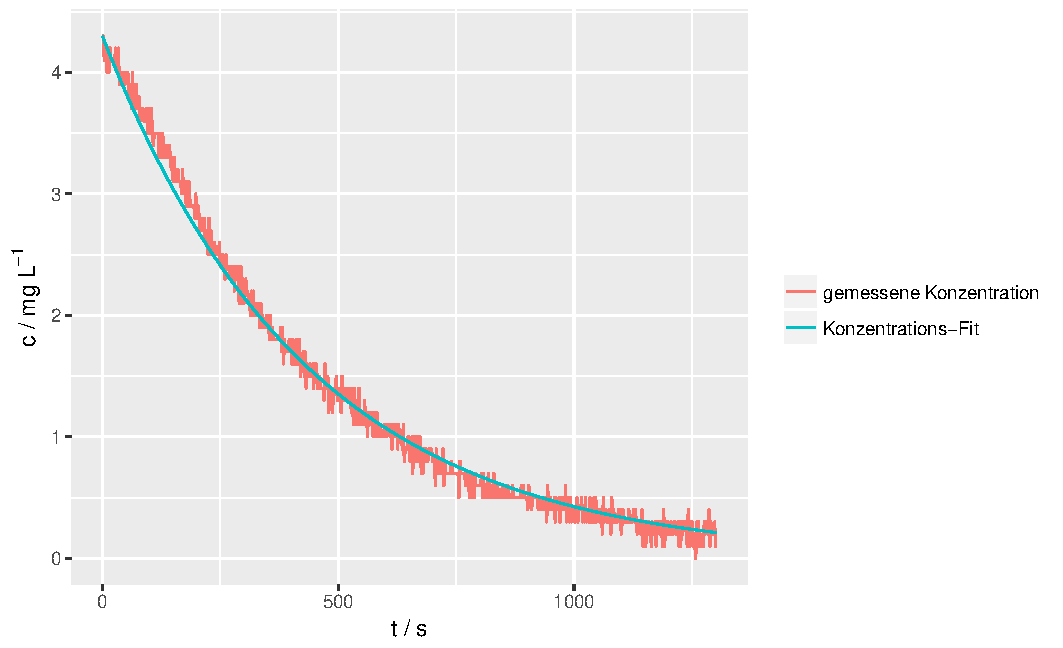
\includegraphics[width=1\textwidth]{Graphics/austreiben_versuch-2.pdf} 
\caption[Austreiben Versuch 2]{tatsächliche und gefittete Konzentration beim Austreiben - Versuch 2}
\label{fig:c_aus_versuch2}
\end{figure}
\noindent

\begin{figure}[H]
\centering
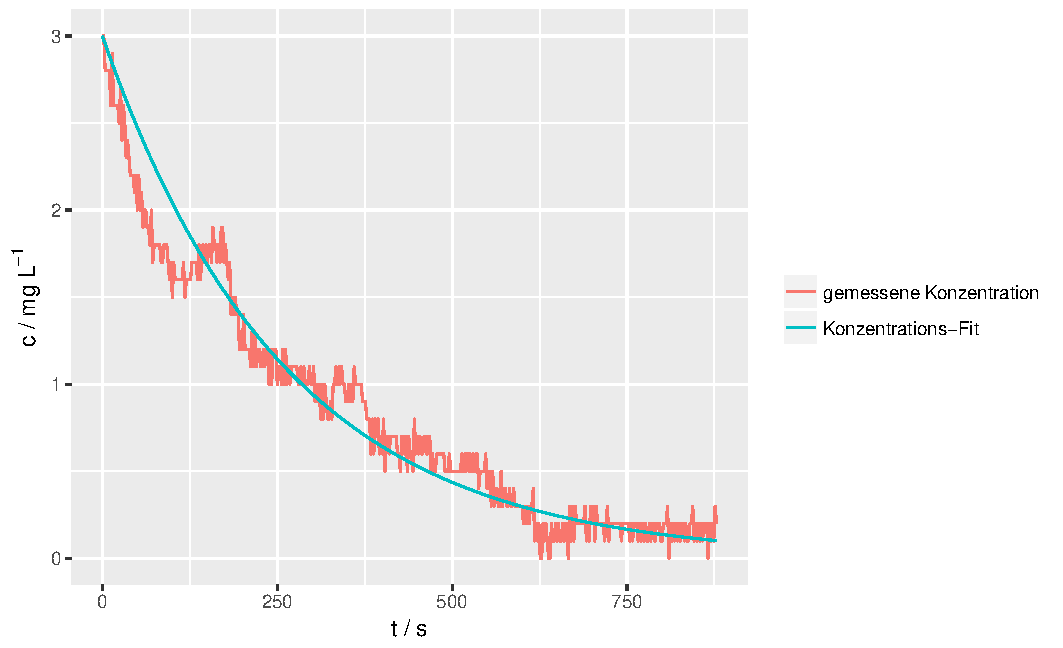
\includegraphics[width=1\textwidth]{Graphics/austreiben_versuch-3.pdf} 
\caption[Austreiben Versuch 3]{tatsächliche und gefittete Konzentration beim Austreiben - Versuch 3}
\label{fig:c_aus_versuch3}
\end{figure}
\noindent

\begin{figure}[H]
\centering
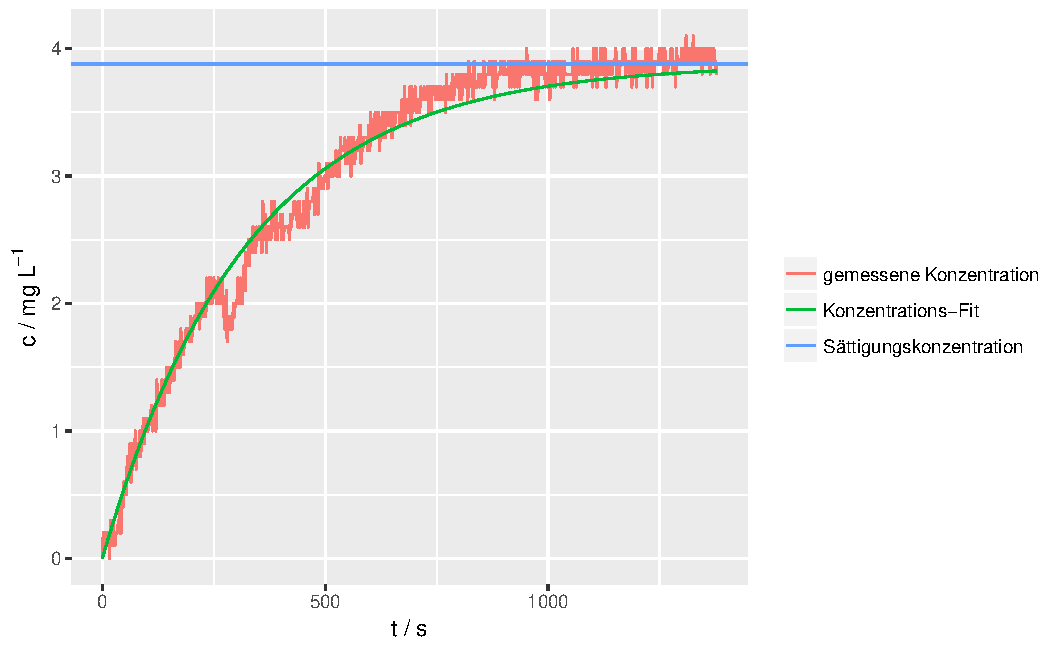
\includegraphics[width=1\textwidth]{Graphics/aufsaettigen_versuch-2.pdf} 
\caption[Aufsättigen Versuch 2]{tatsächliche und gefittete Konzentration beim Aufsättigen mit angenommener Gleichgewichtskonzentration - Versuch 2}
\label{fig:c_auf_versuch2_saett}
\end{figure}
\noindent

\begin{figure}[H]
\centering
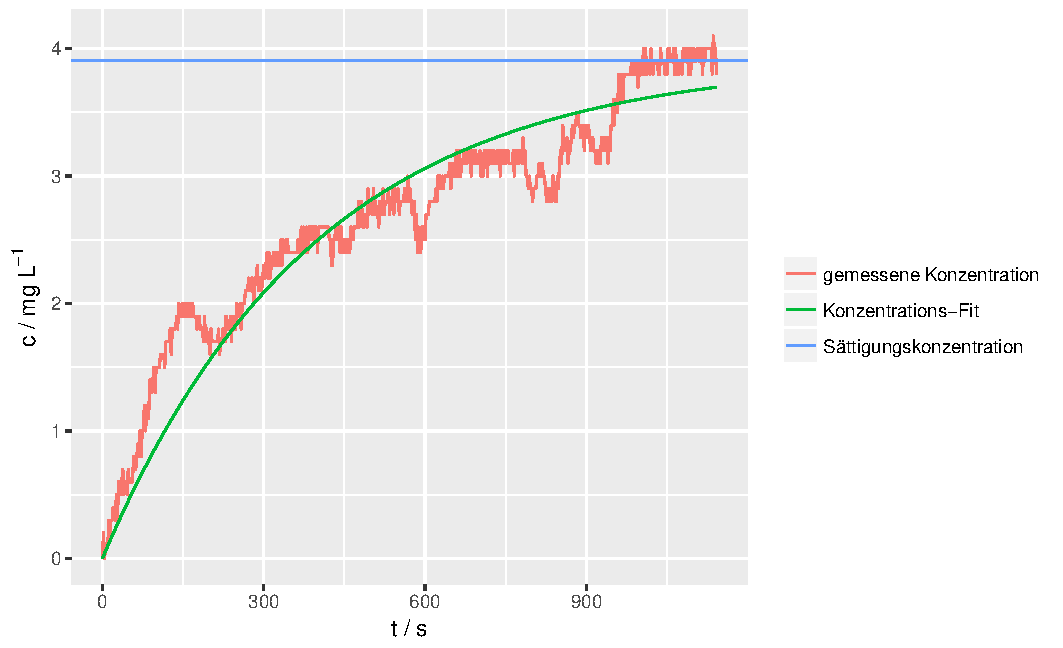
\includegraphics[width=1\textwidth]{Graphics/aufsaettigen_versuch-3.pdf} 
\caption[Aufsättigen Versuch 3]{tatsächliche und gefittete Konzentration beim Aufsättigen mit angenommener Gleichgewichtskonzentration - Versuch 3}
\label{fig:c_auf_versuch3_saett}
\end{figure}
\noindent

\begin{figure}[H]
\begin{center}
	\subfigure[Bild 1]{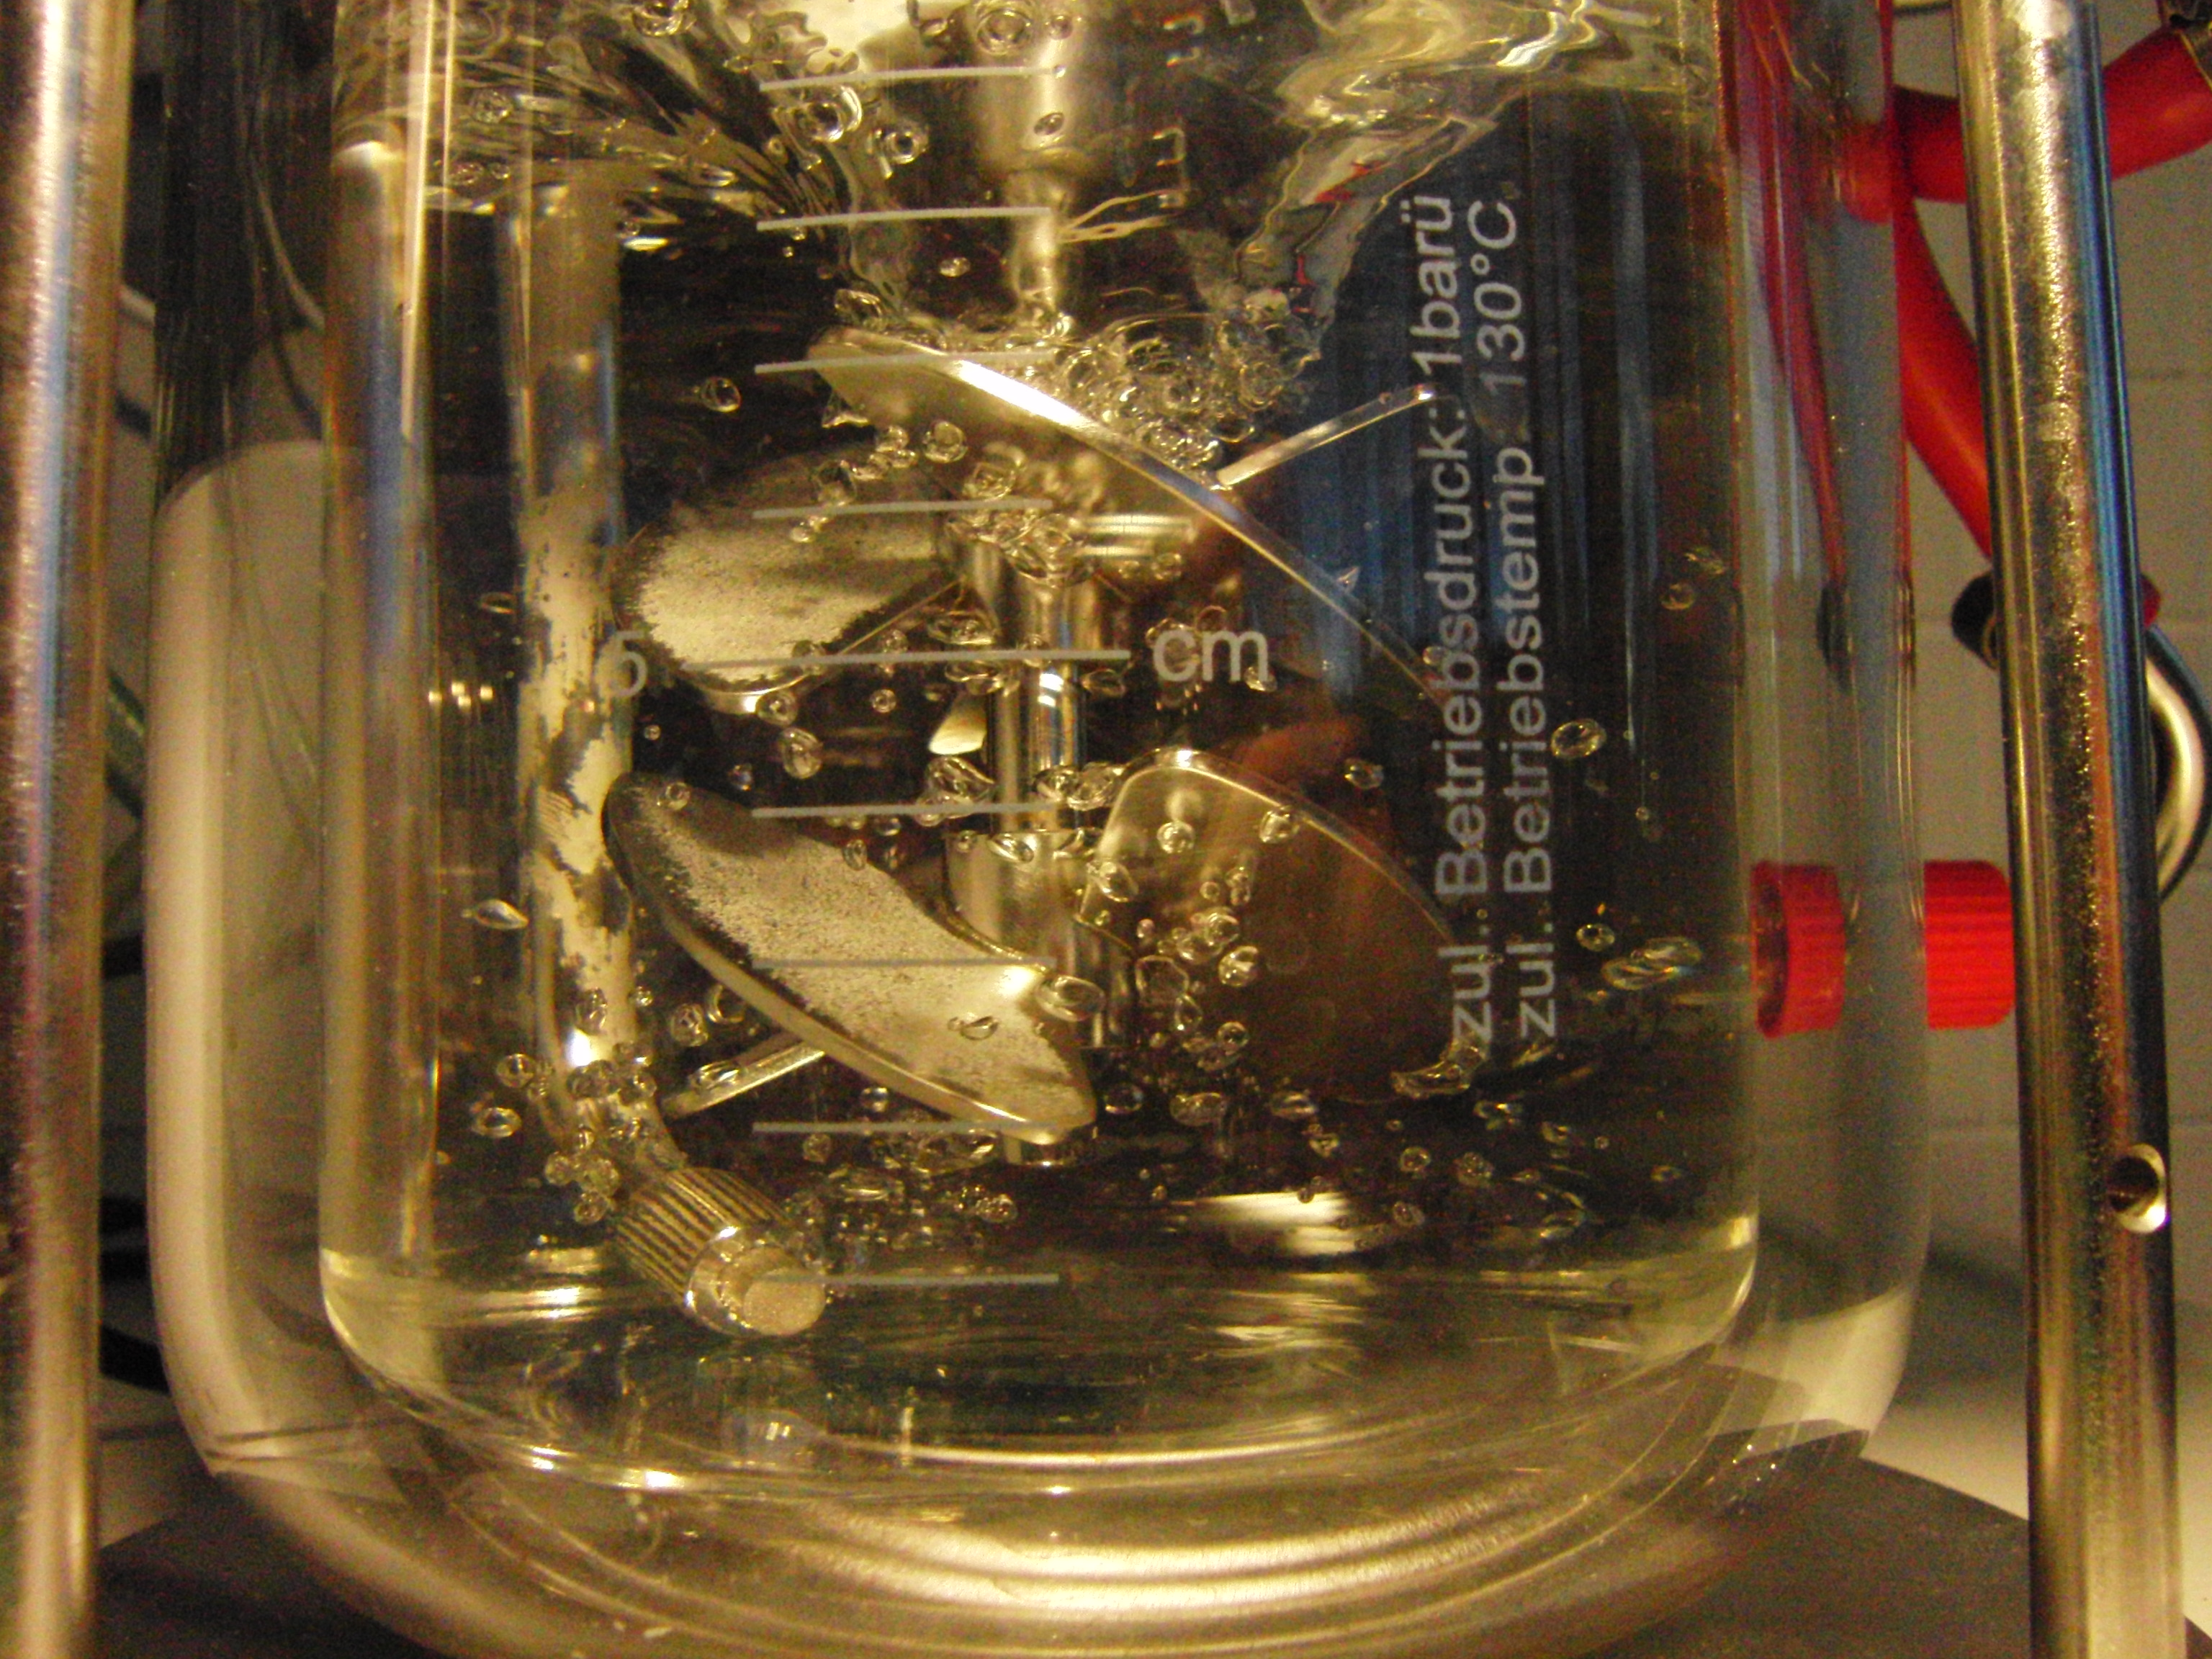
\includegraphics[height=4cm]{Blasenmessung/Versuch_2_1.JPG}}\label{blasengroesse1}
	\hspace{1cm}
	\subfigure[Bild 2]{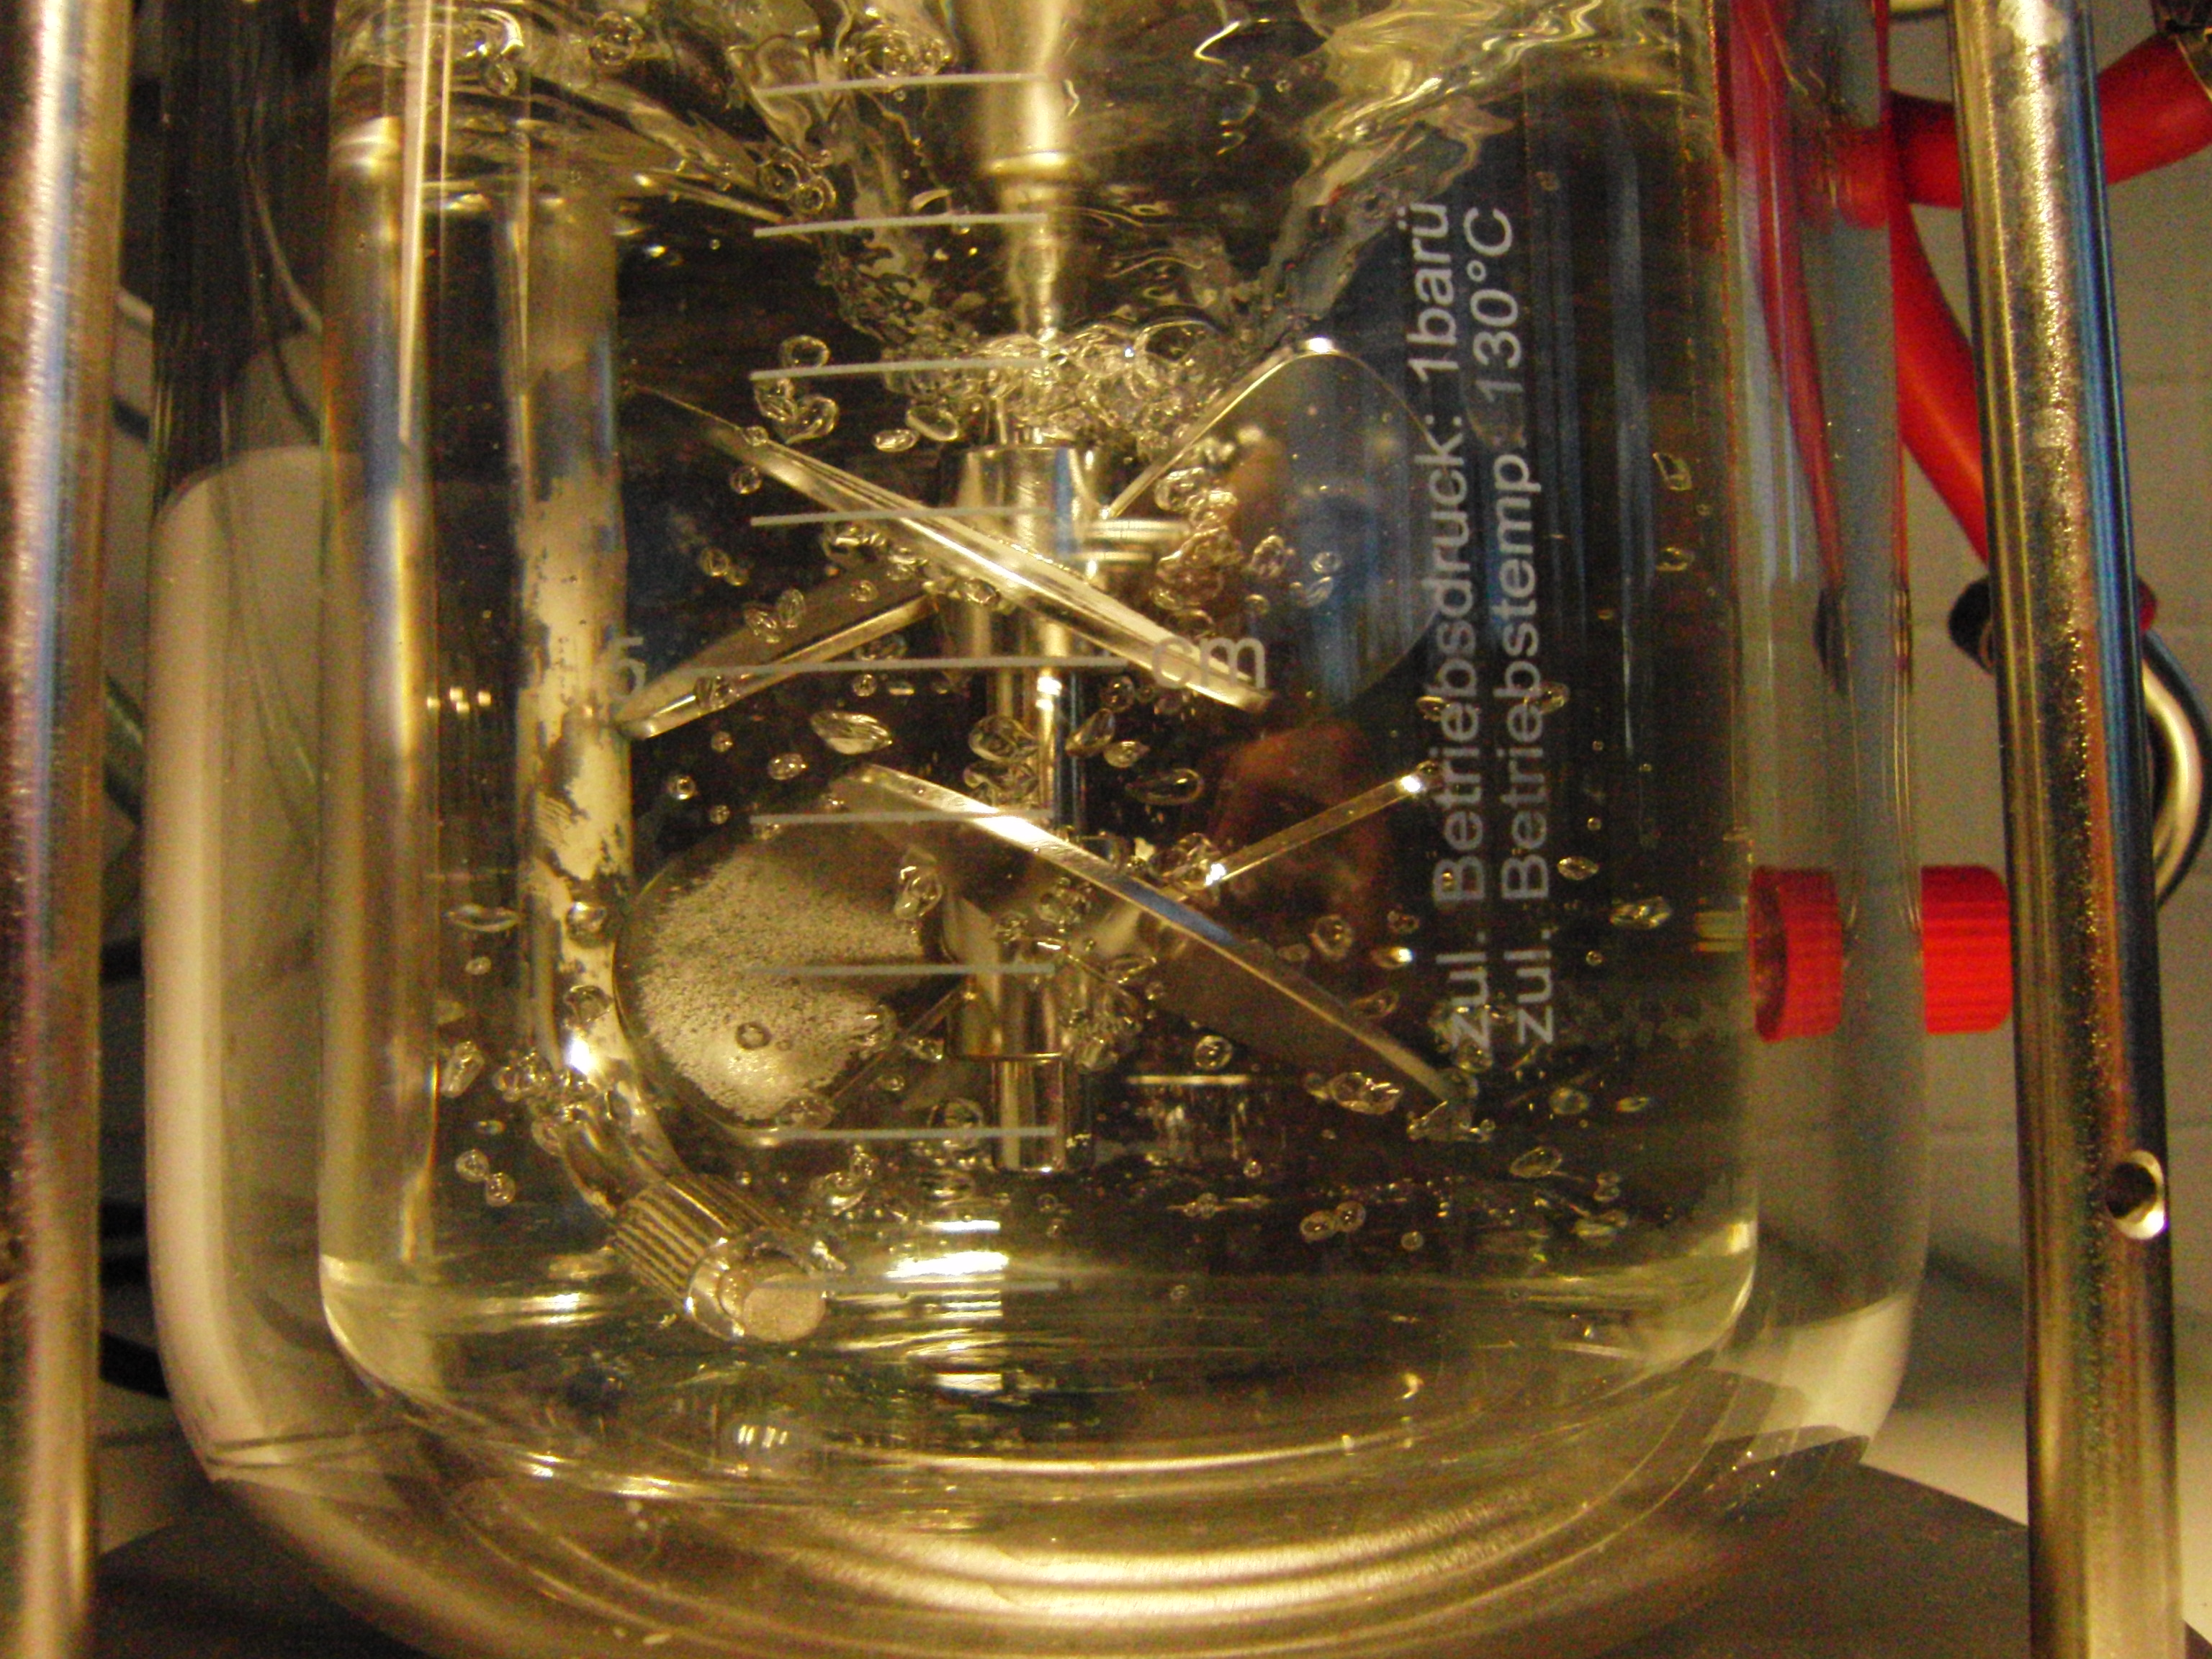
\includegraphics[height=4cm]{Blasenmessung/Versuch_2_2.JPG}}\label{blasengroesse2}
	\hspace{1cm}
	\subfigure[Bild 3]{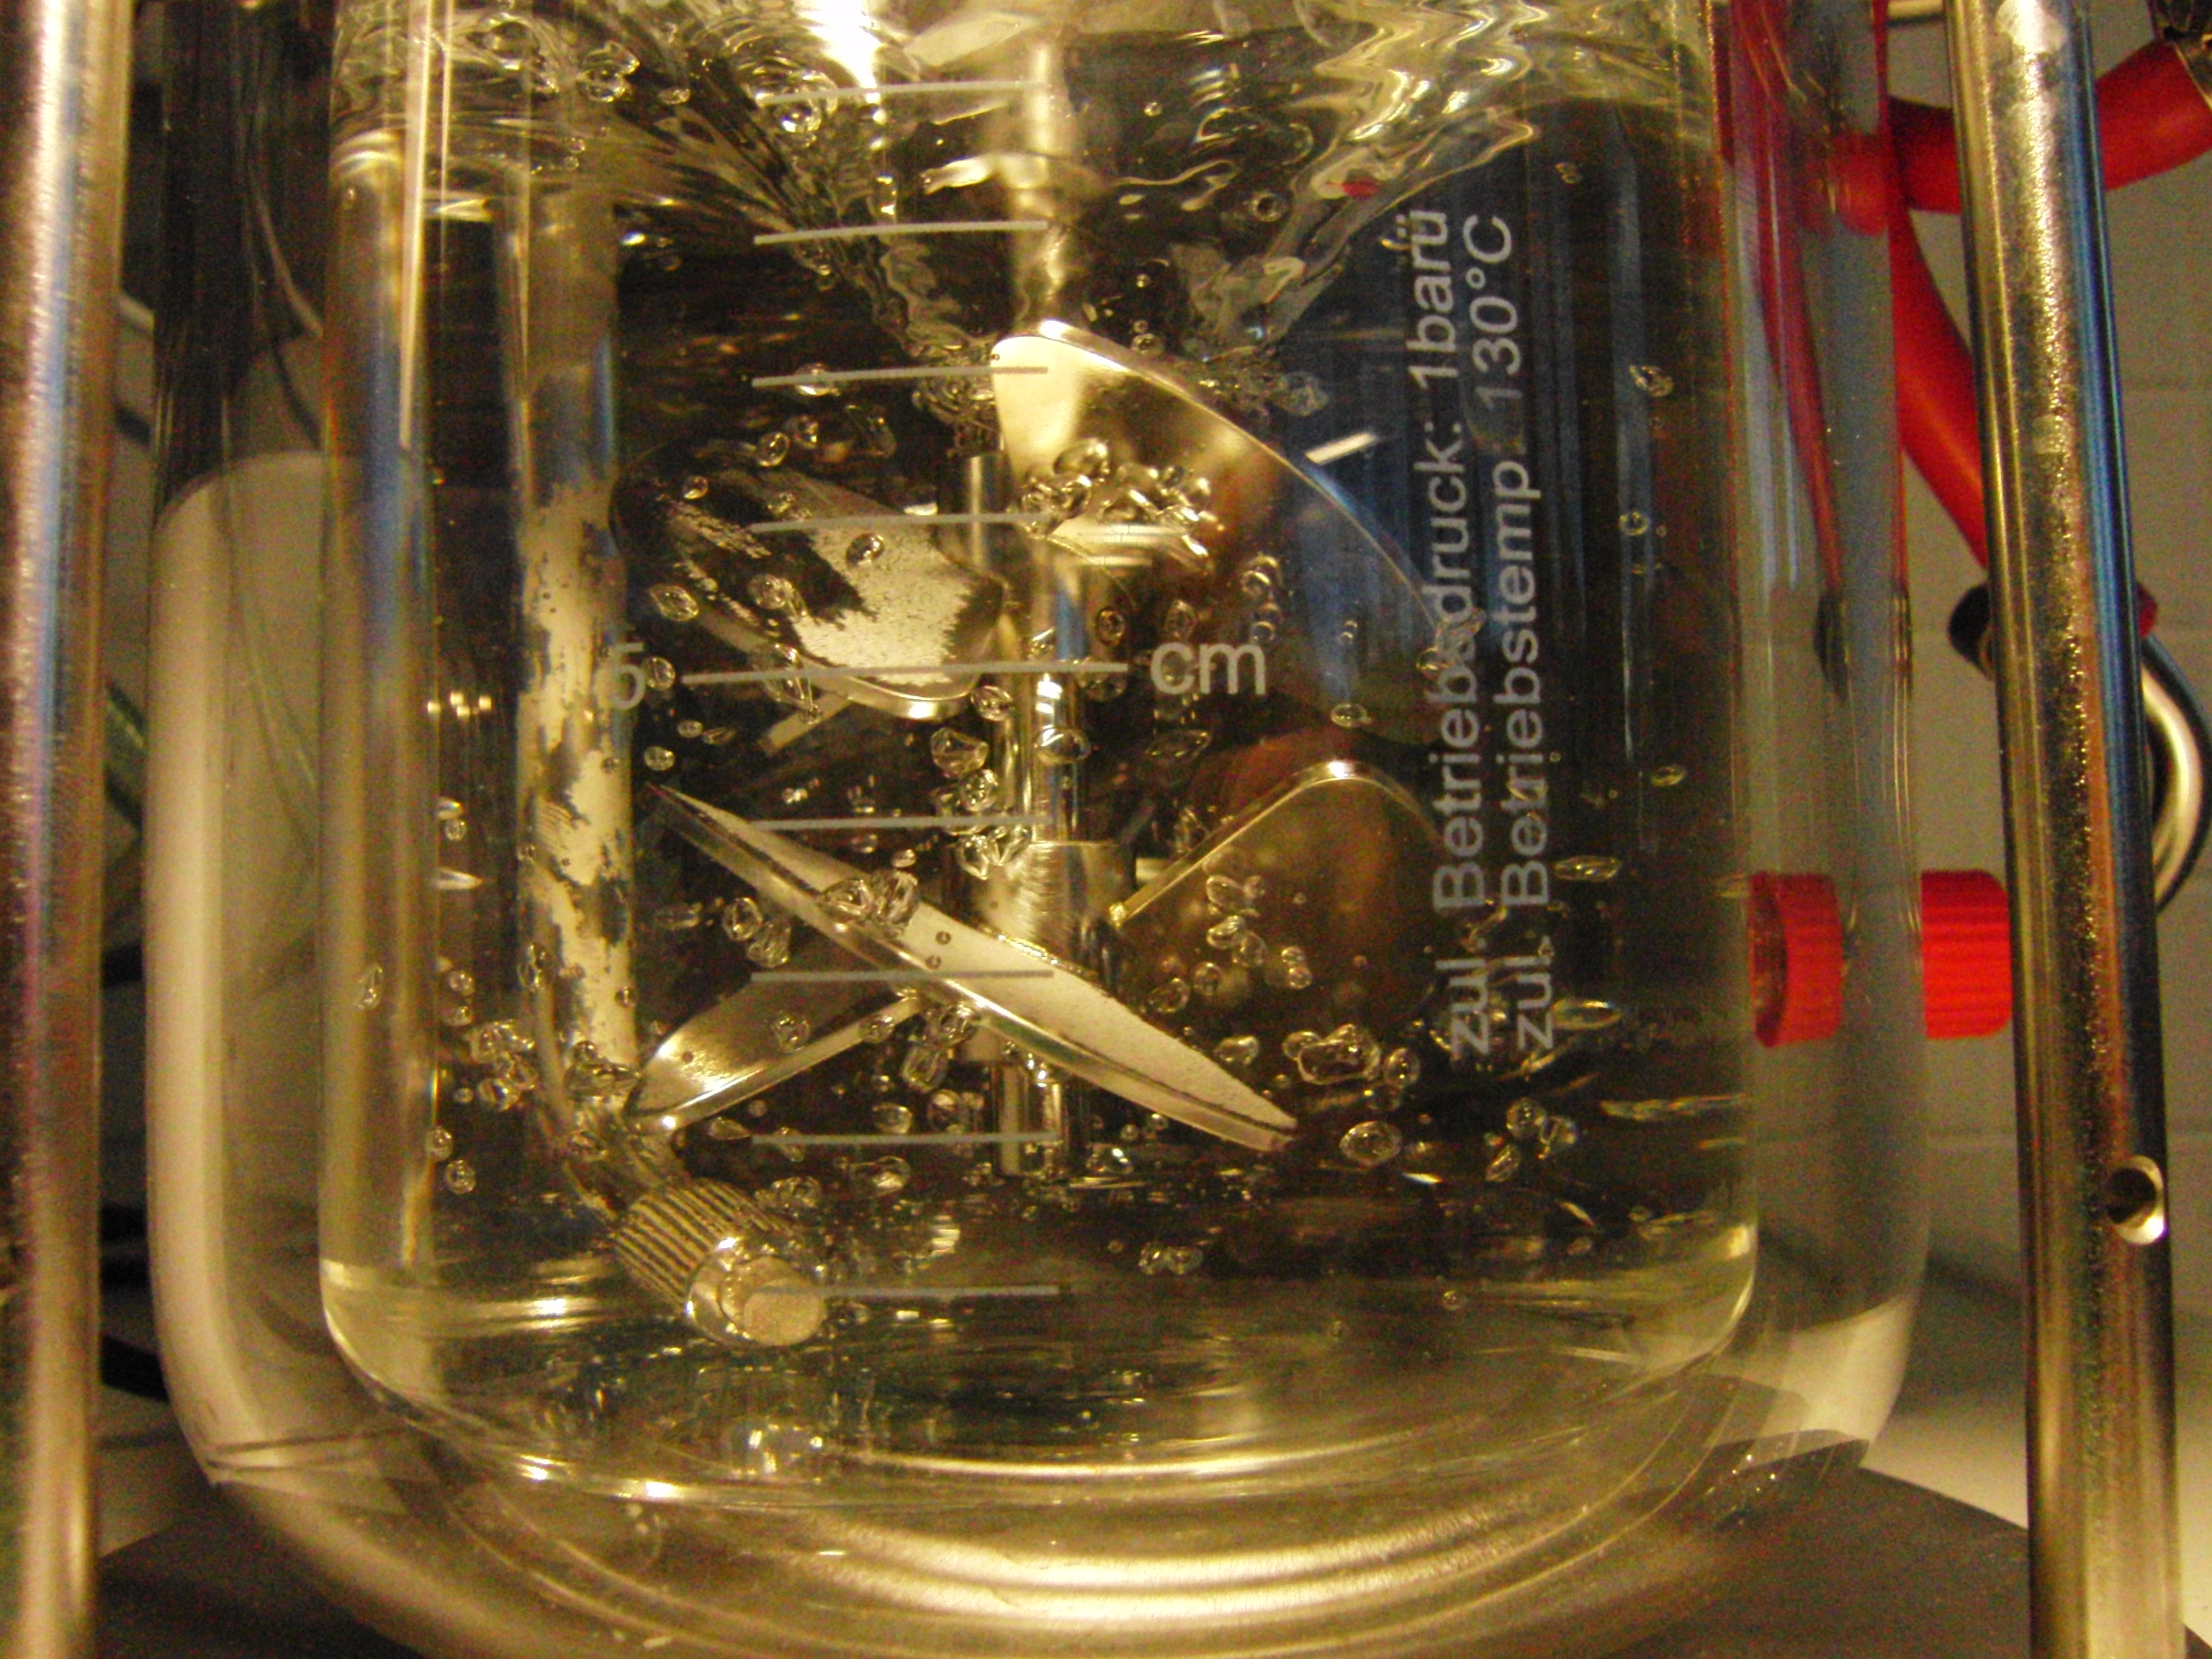
\includegraphics[height=4cm]{Blasenmessung/Versuch_2_3.JPG}}\label{blasengroesse3}
	\hspace{1cm}
	\subfigure[Bild 4]{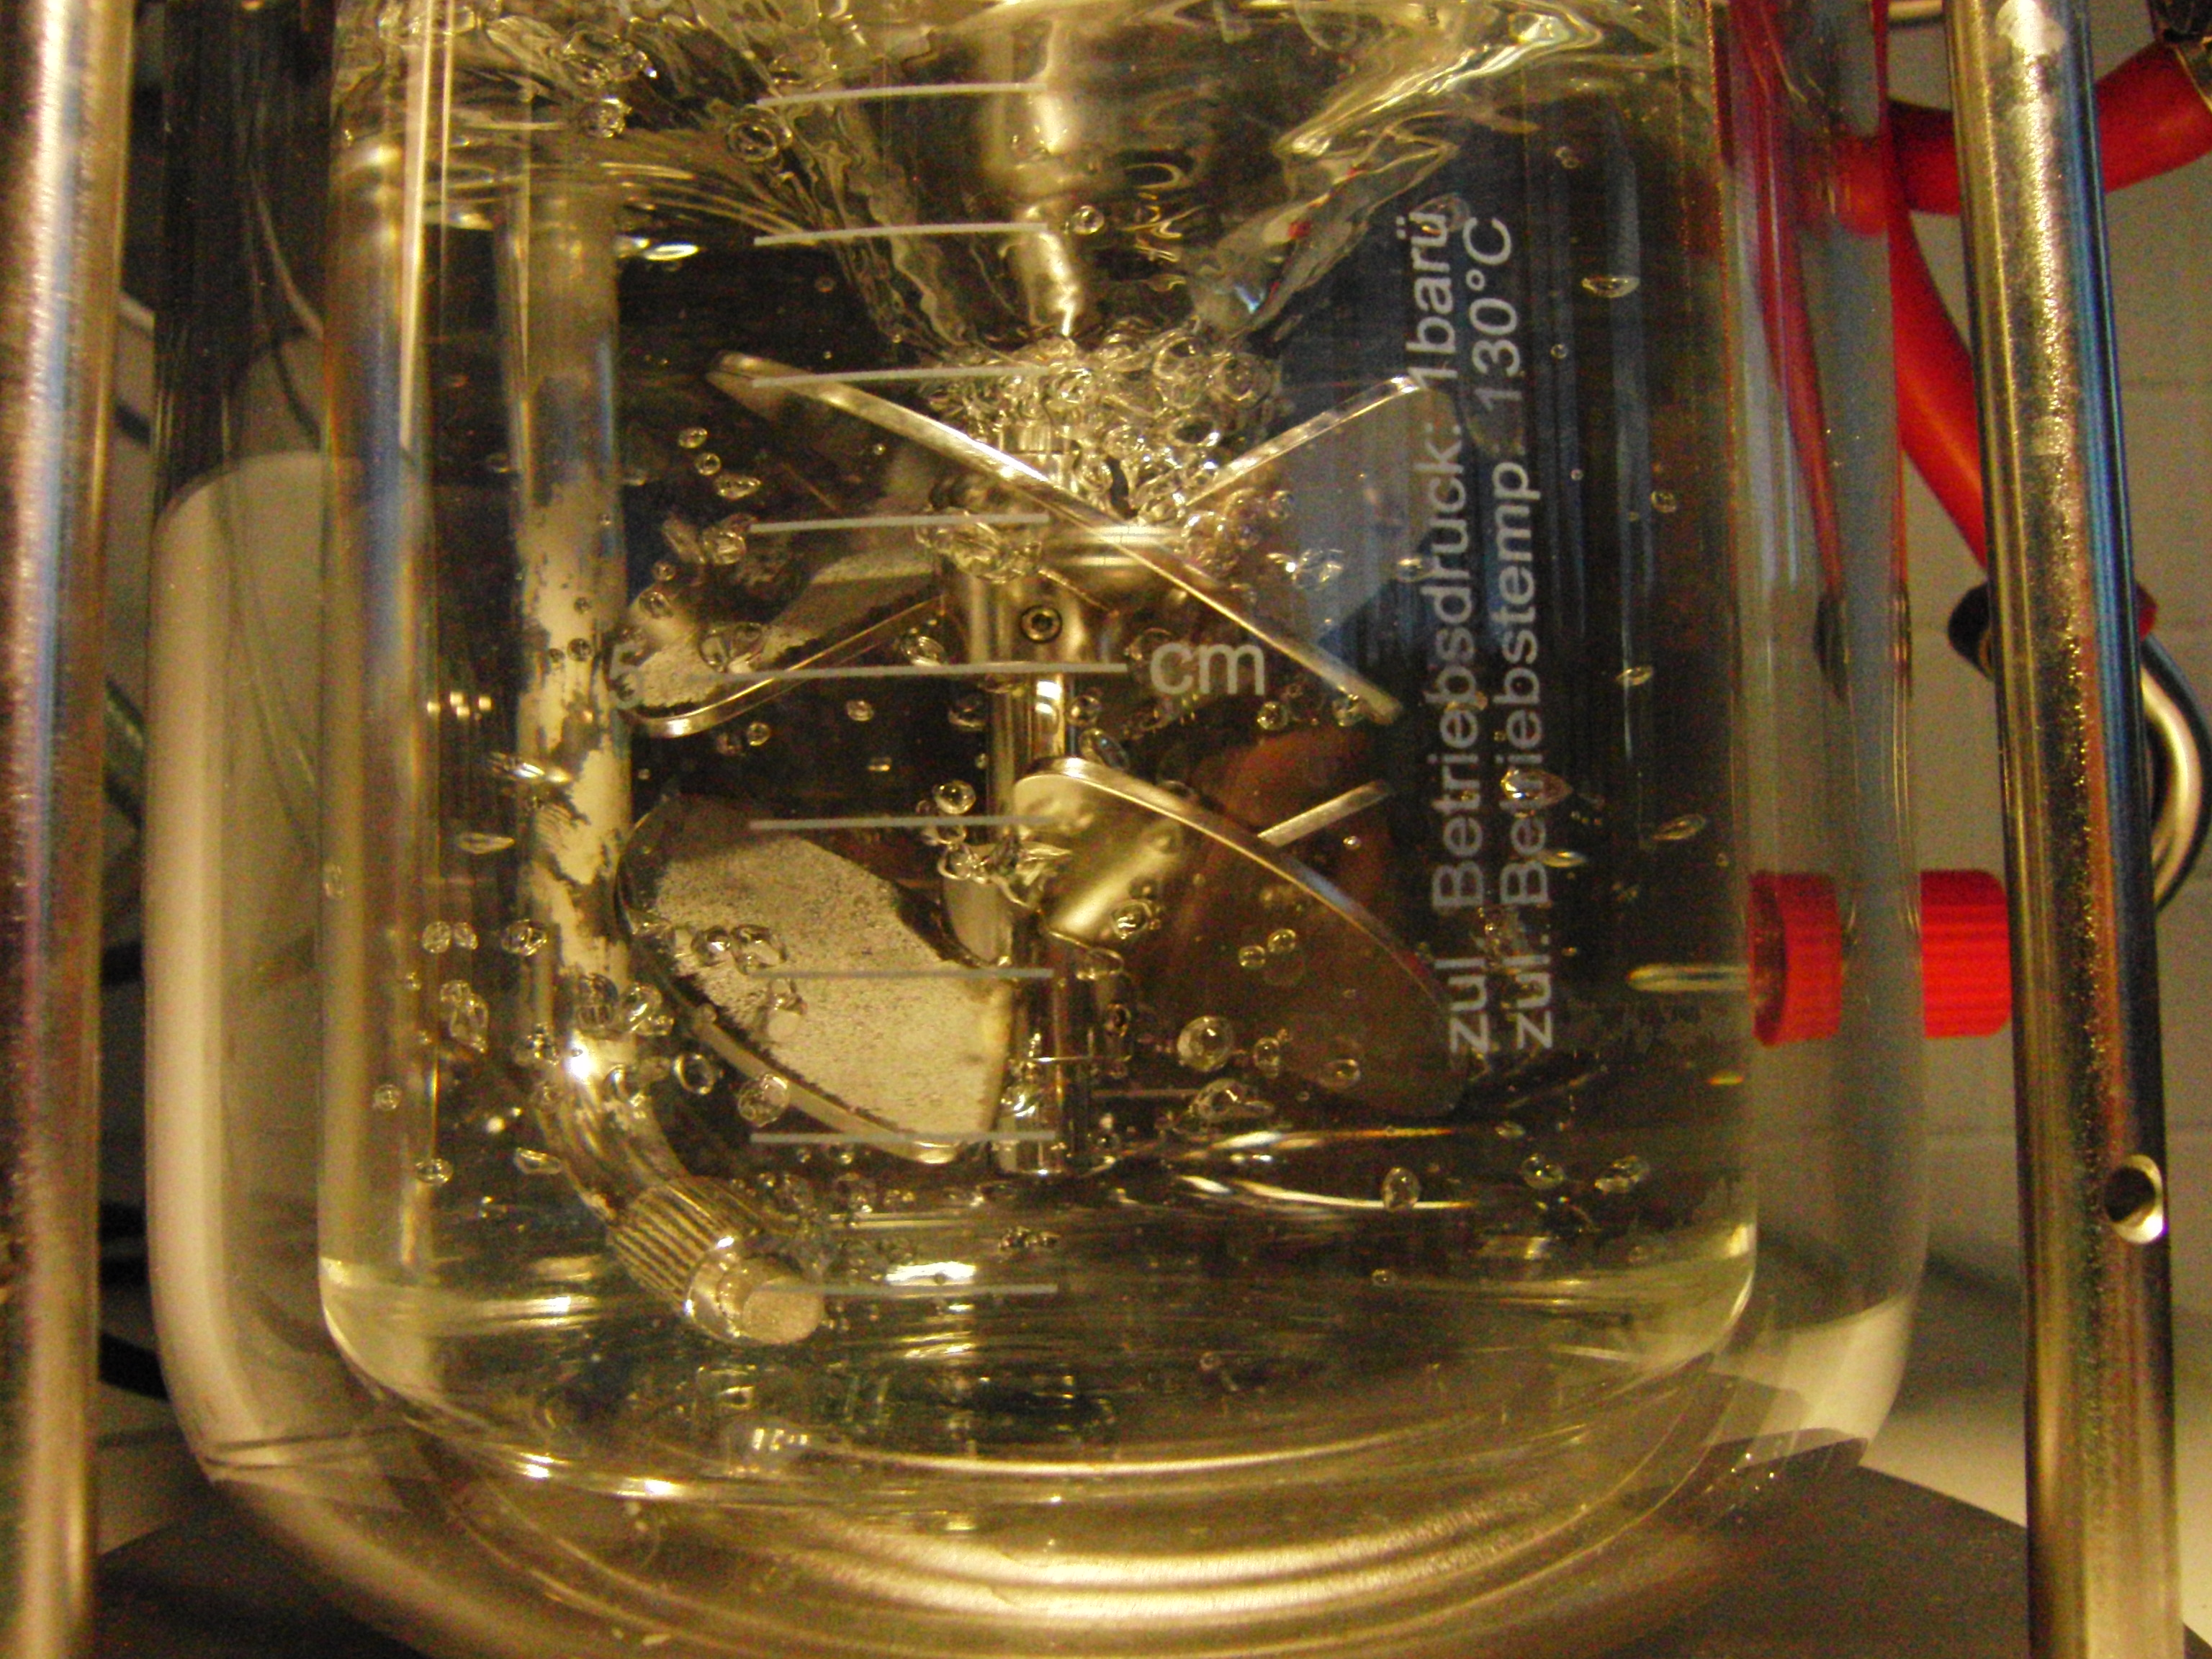
\includegraphics[height=4cm]{Blasenmessung/Versuch_2_4.JPG}}\label{blasengroesse4}
	\hspace{1cm}
	\subfigure[Bild 5]{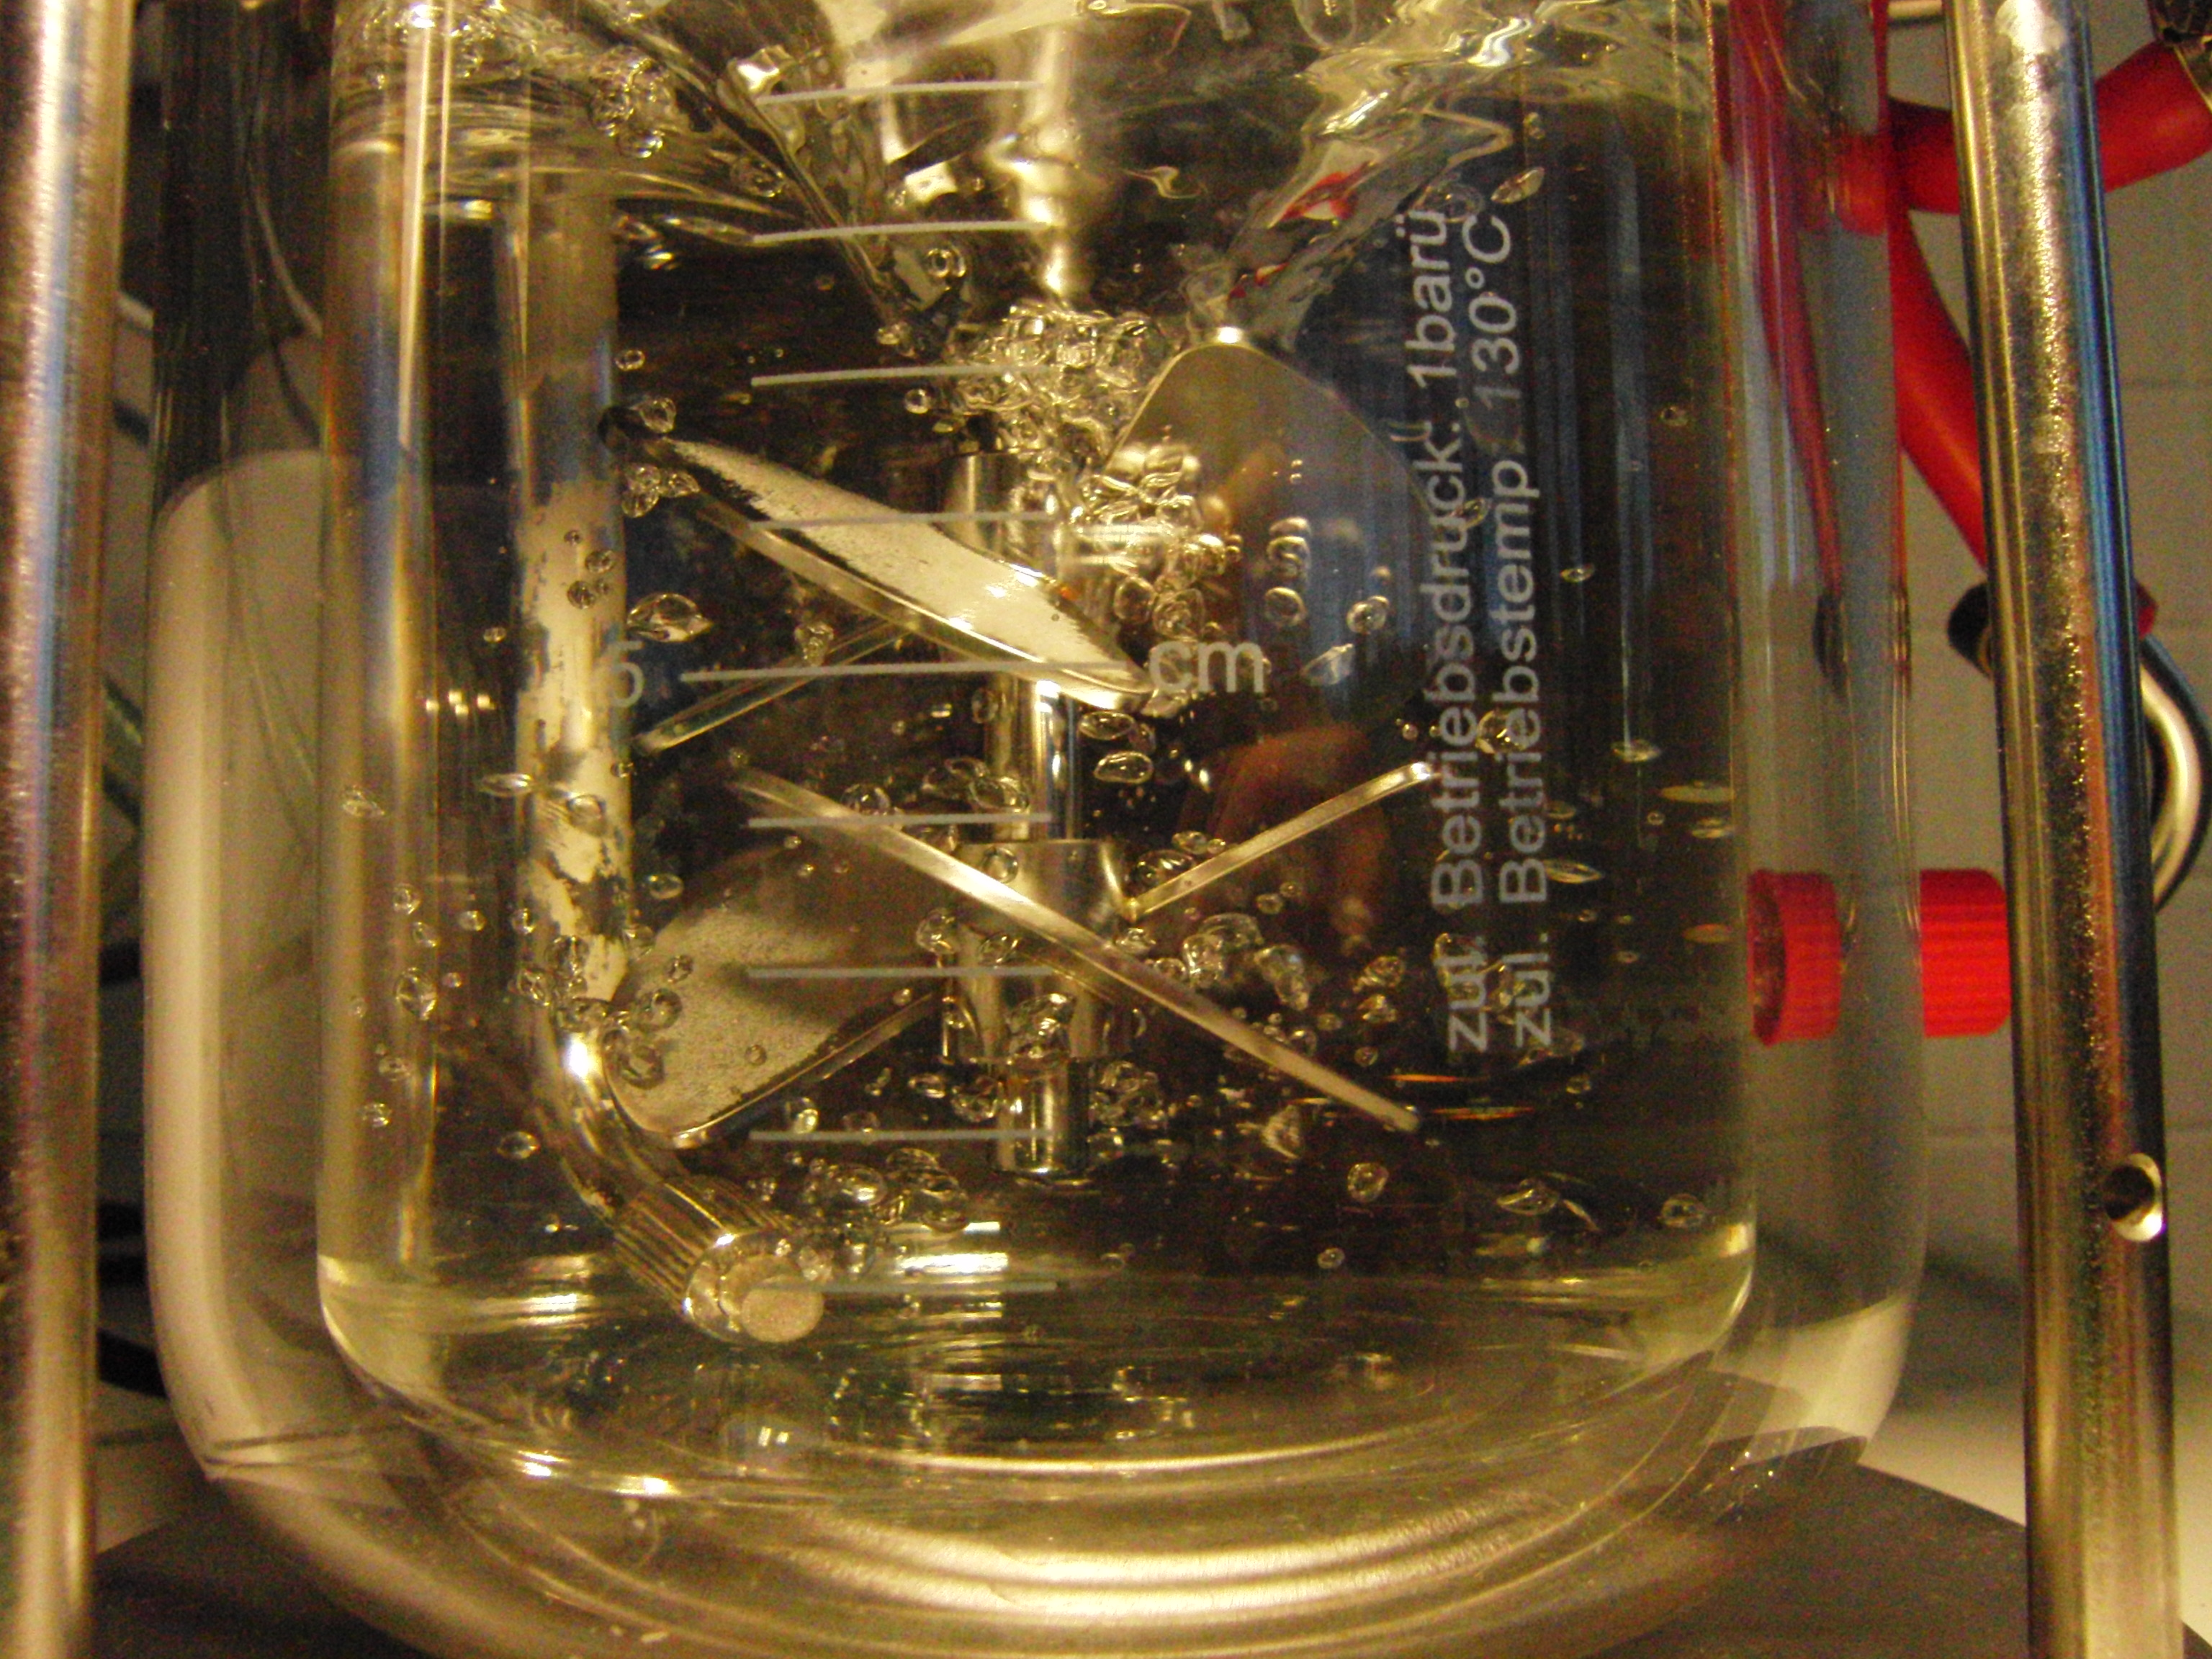
\includegraphics[height=4cm]{Blasenmessung/Versuch_2_5.JPG}}\label{blasengroesse5}
	\hspace{1cm}
	\subfigure[Bild 6]{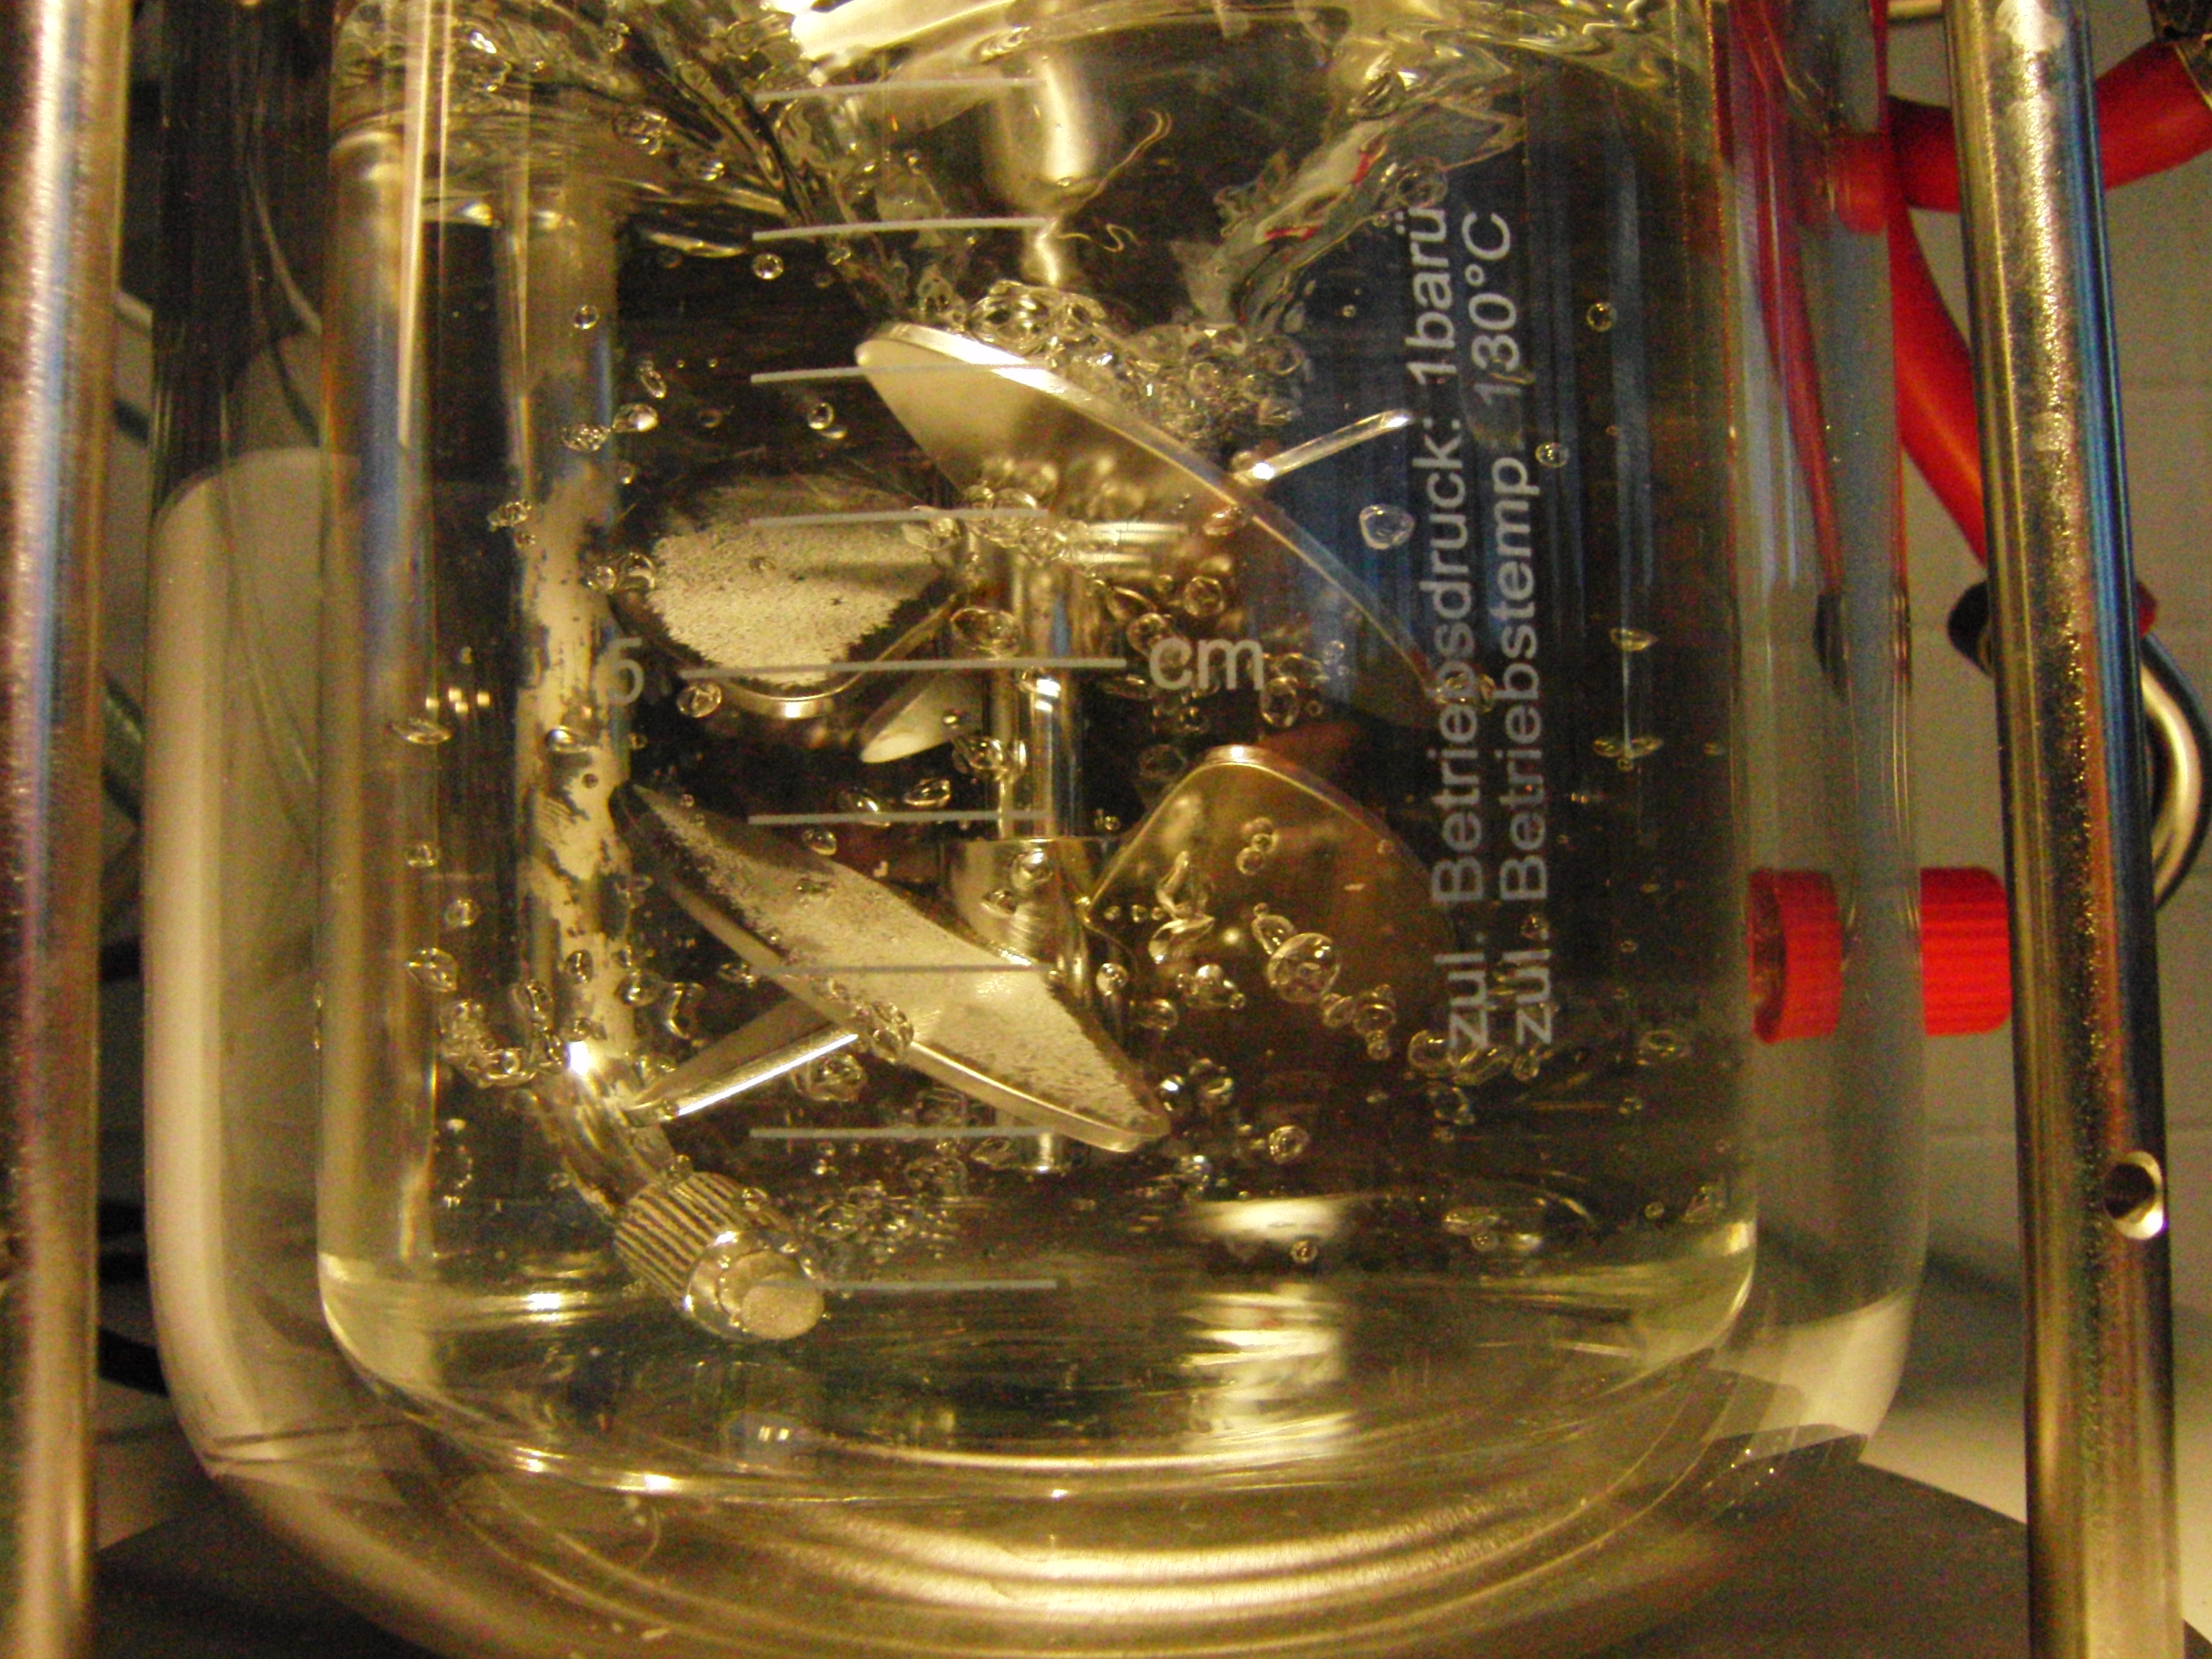
\includegraphics[height=4cm]{Blasenmessung/Versuch_2_6.JPG}}\label{blasengroesse6}
	\hspace{1cm}
	\subfigure[Bild 7]{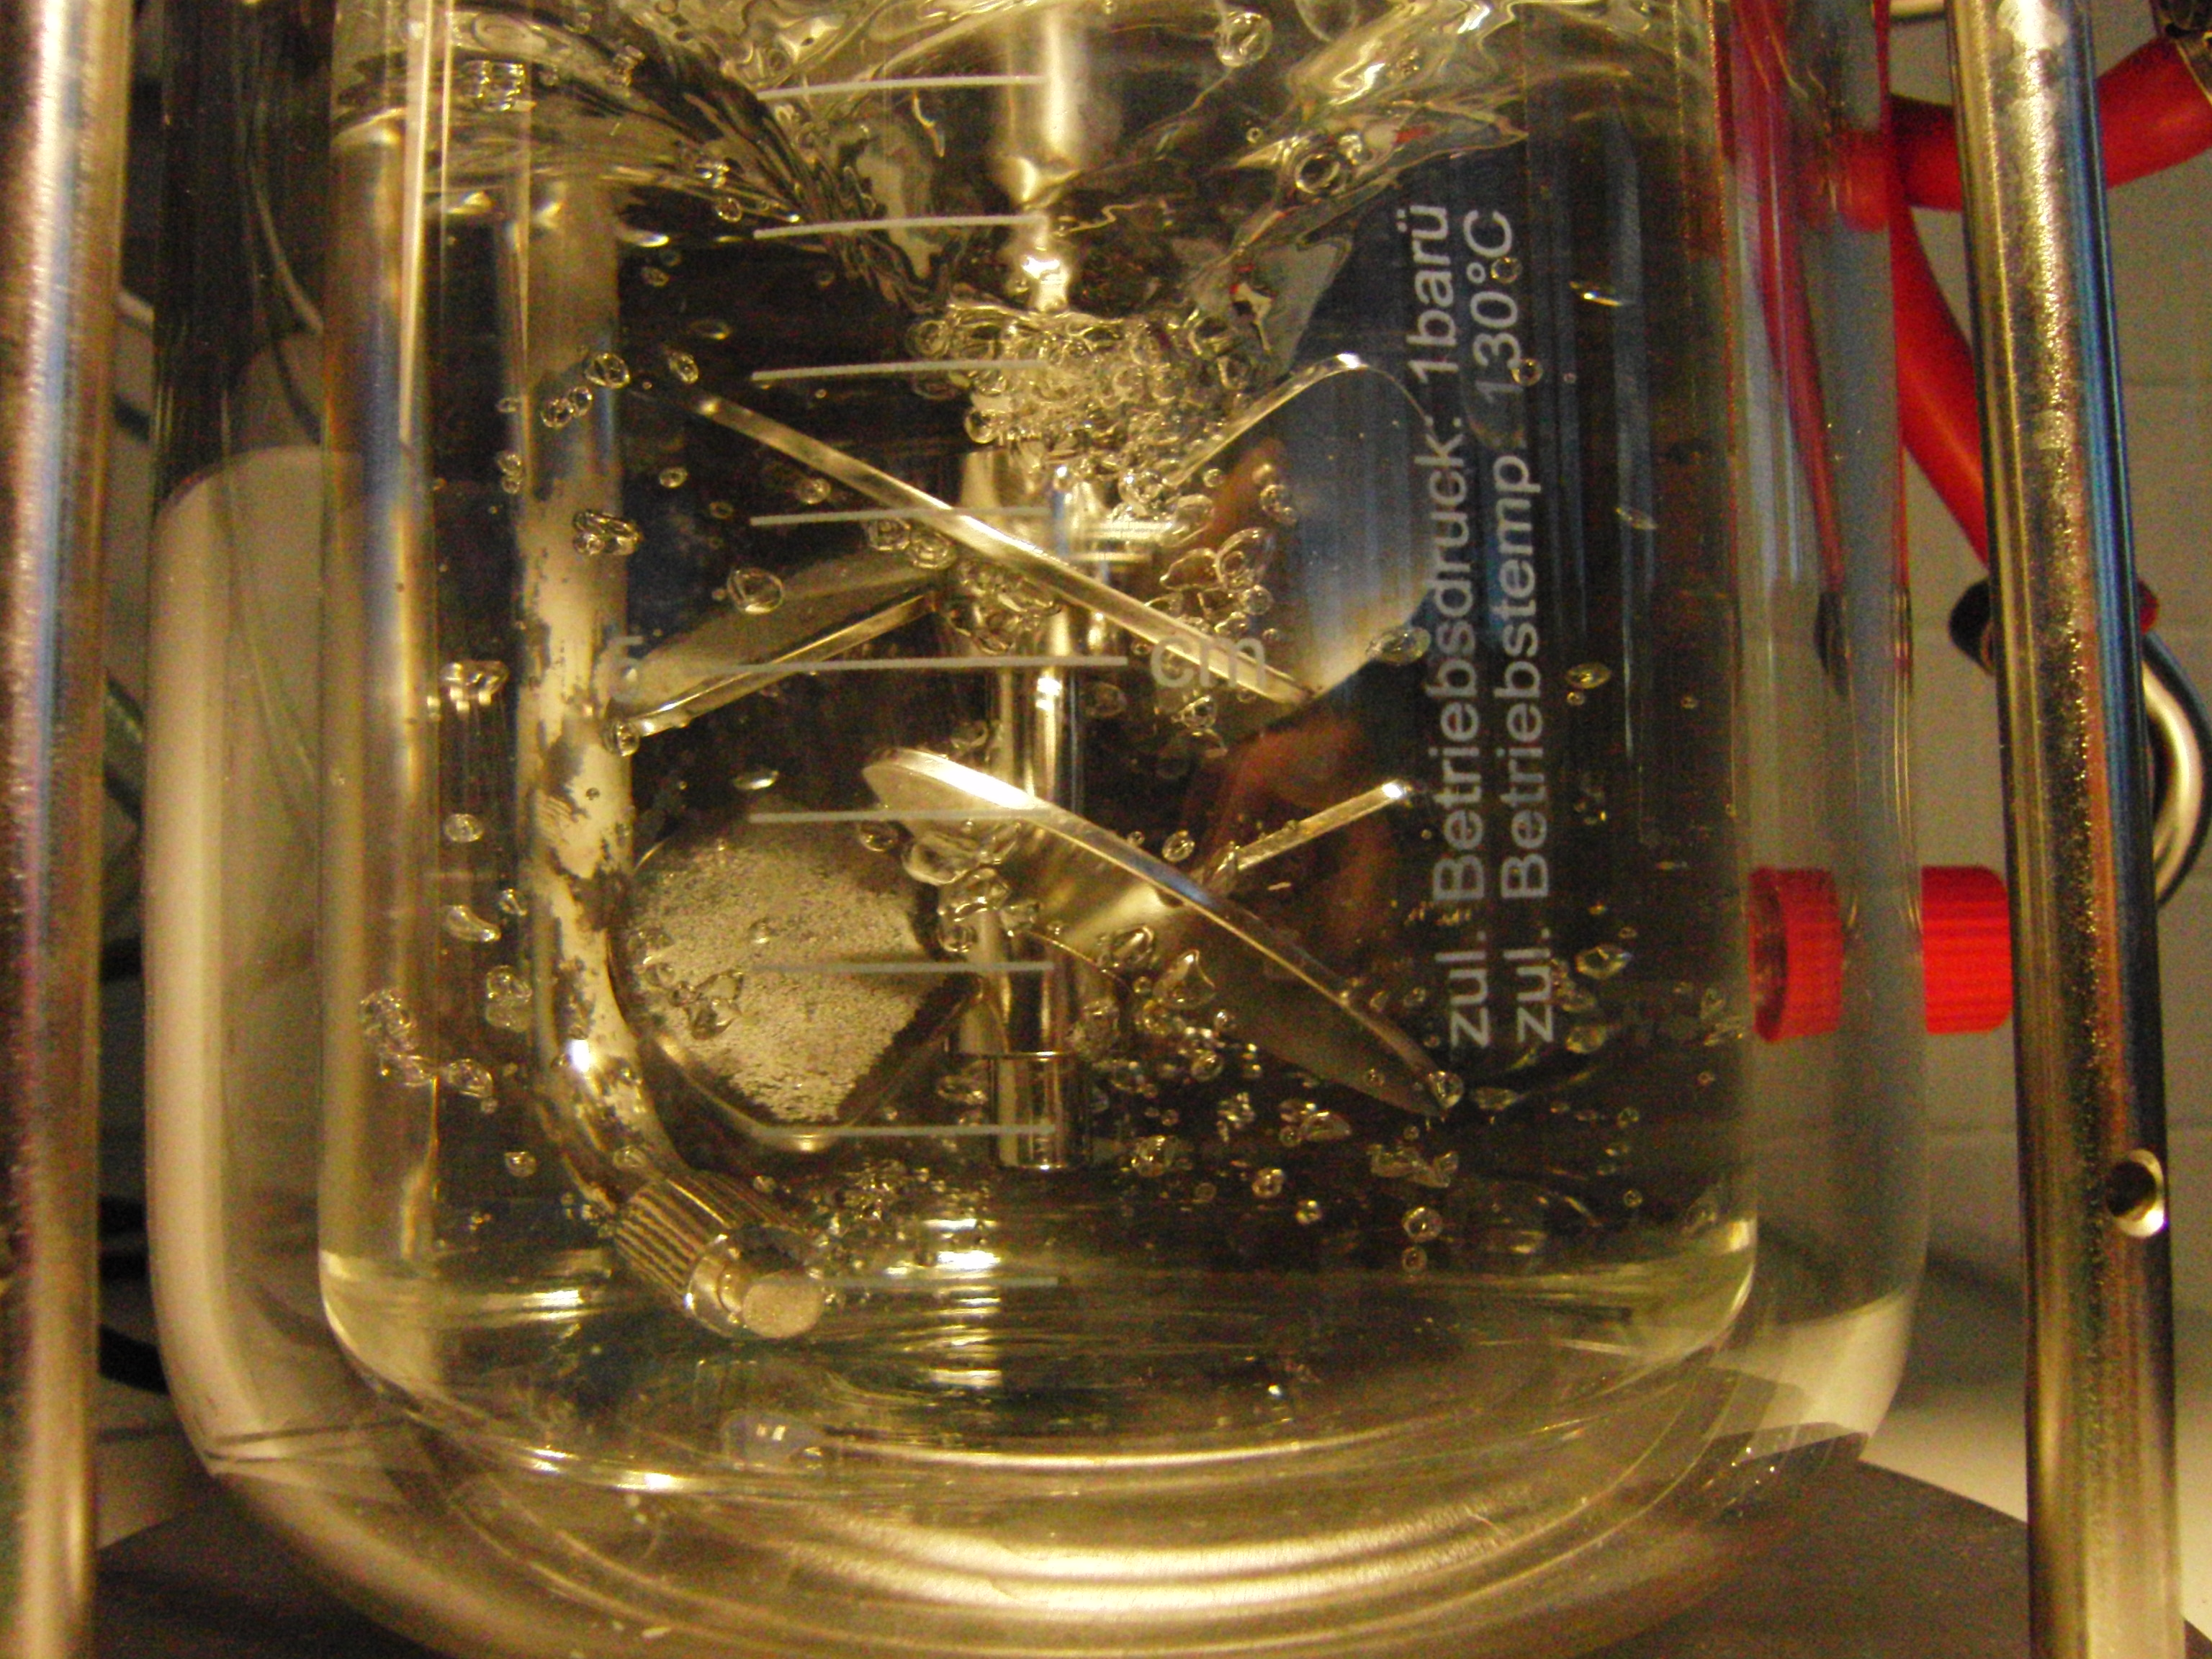
\includegraphics[height=4cm]{Blasenmessung/Versuch_2_7.JPG}}\label{blasengroesse6}
	\hspace{1cm}
	\subfigure[Bild 8]{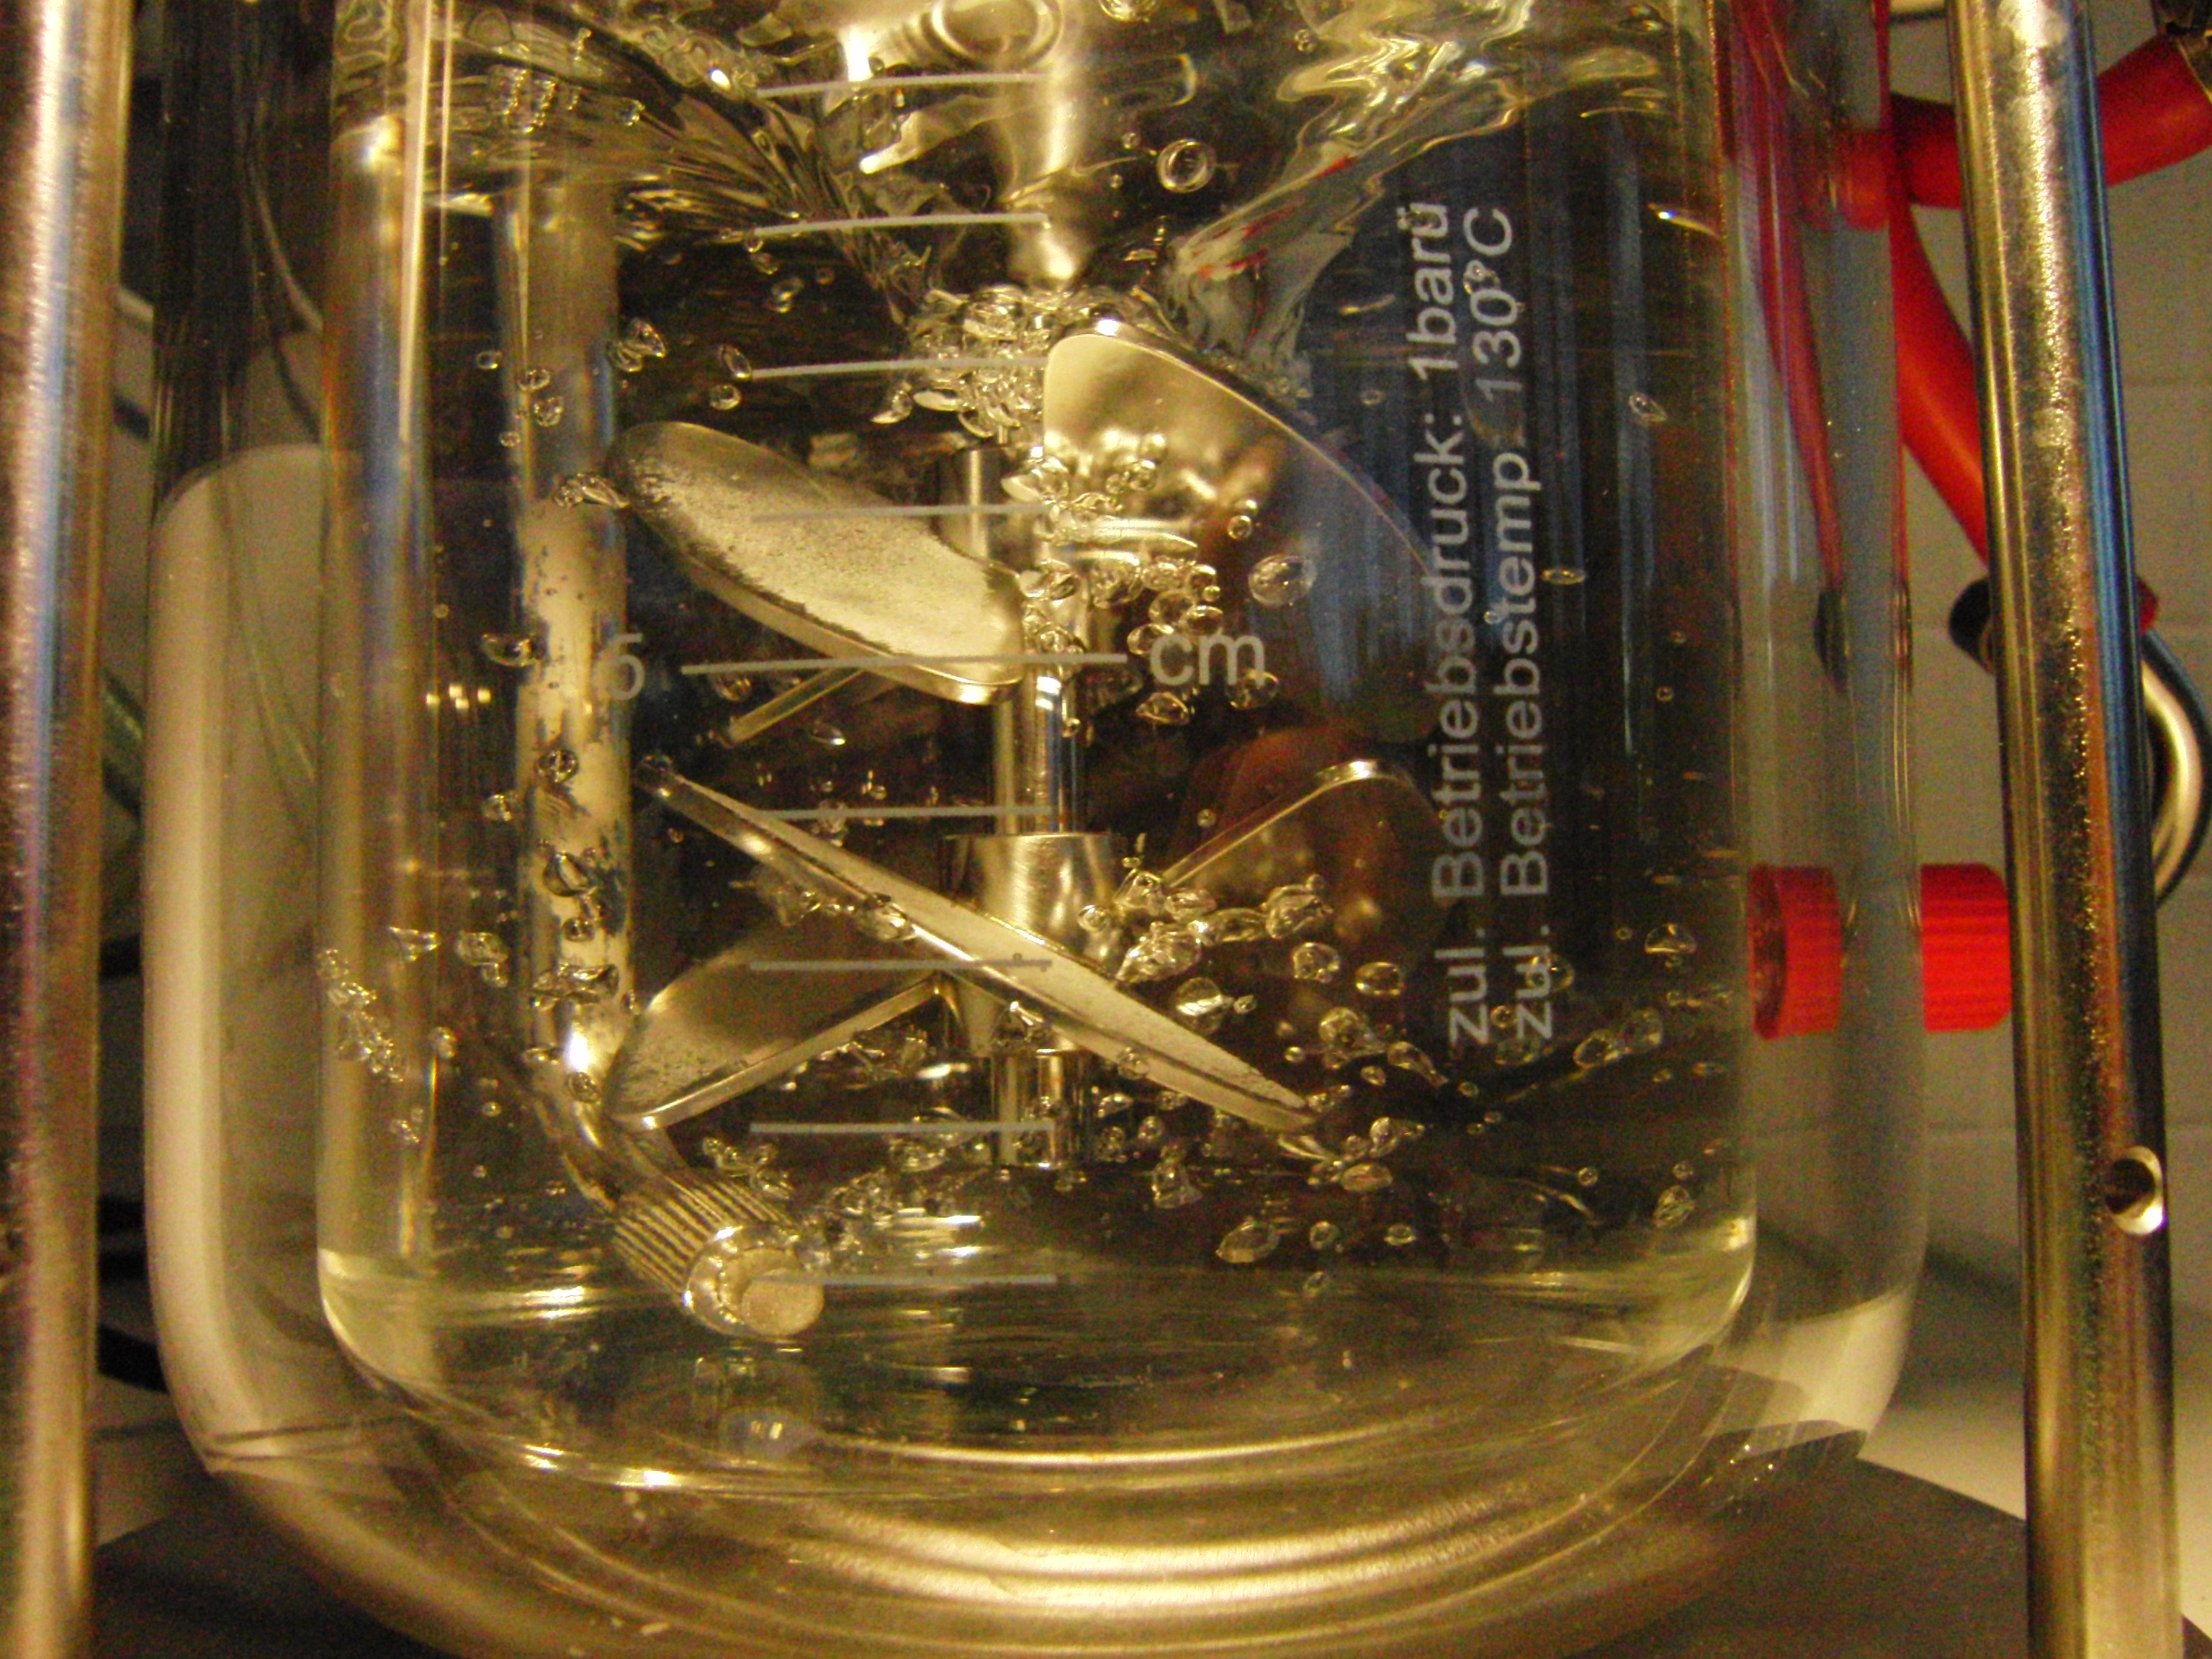
\includegraphics[height=4cm]{Blasenmessung/Versuch_2_8.JPG}}\label{blasengroesse6}
	\caption{Analyse der Blasengröße für Versuch Nr. 2}
	\label{blasengroesseversuch2}
\end{center}	
\end{figure}
\noindent

\begin{figure}[H]
\begin{center}
	\subfigure[Bild 1]{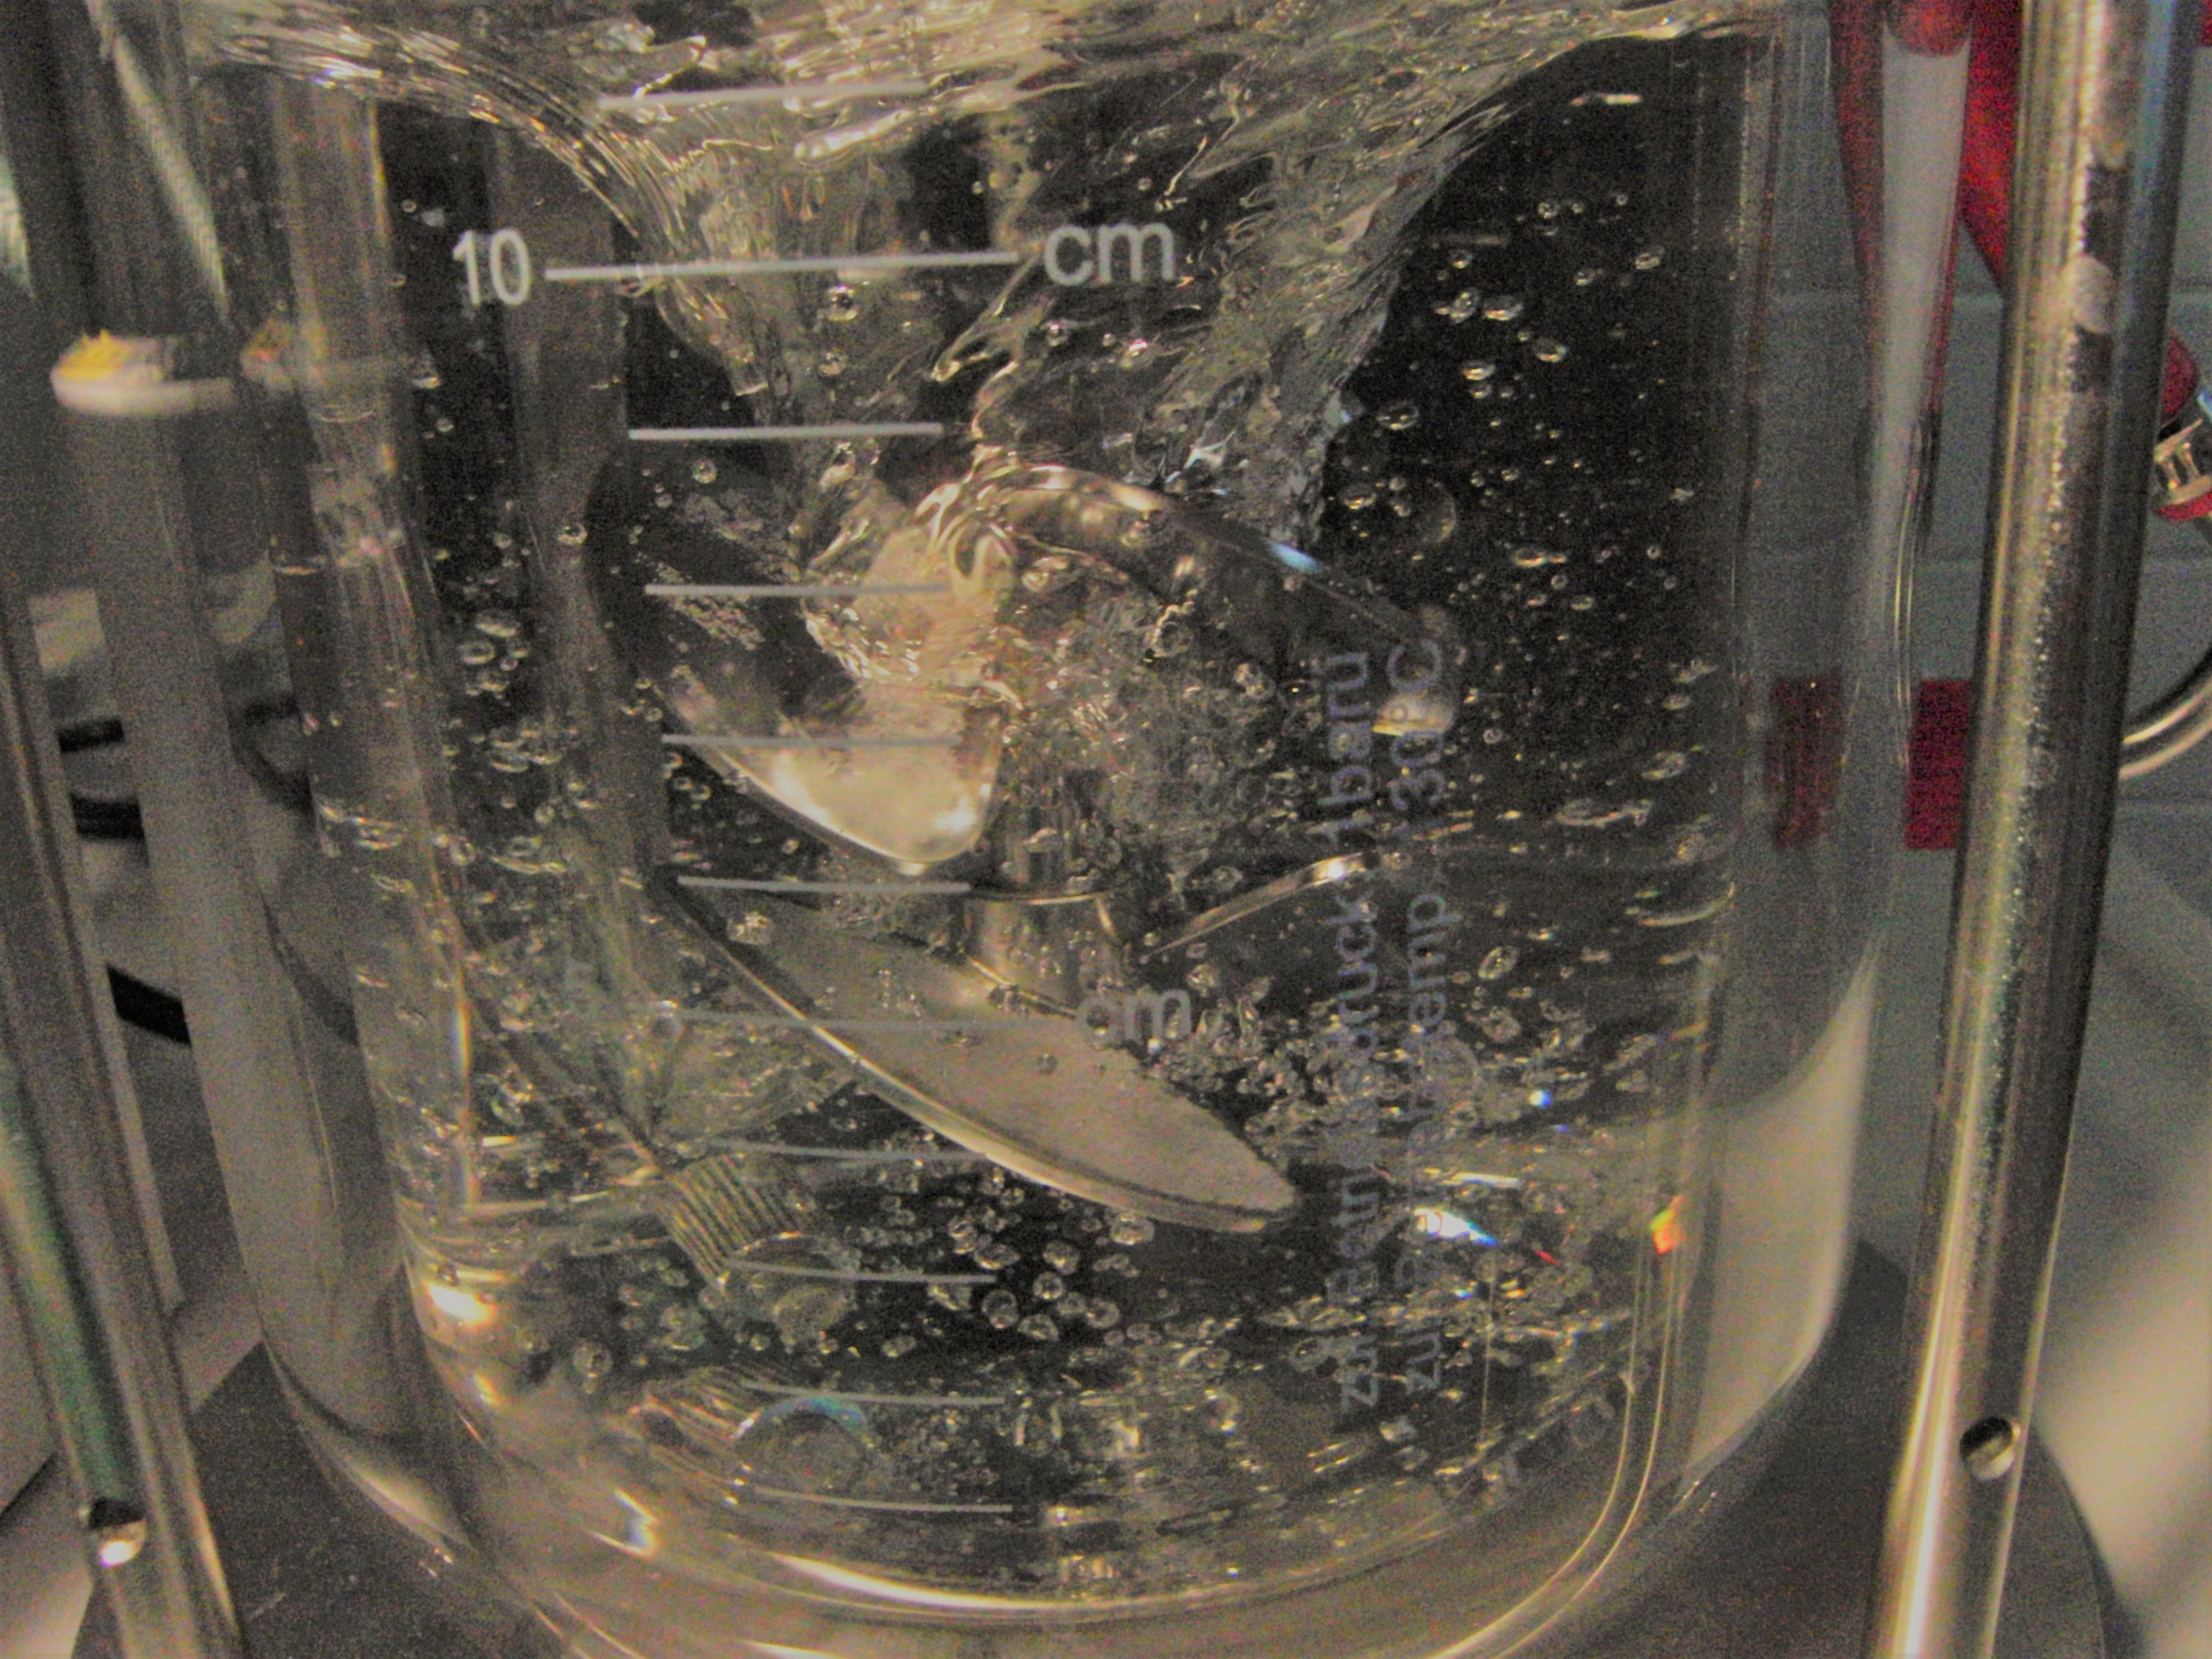
\includegraphics[height=4cm]{Blasenmessung/Versuch_3_1.JPG}}\label{blasengroesse31}
	\hspace{1cm}
	\subfigure[Bild 2]{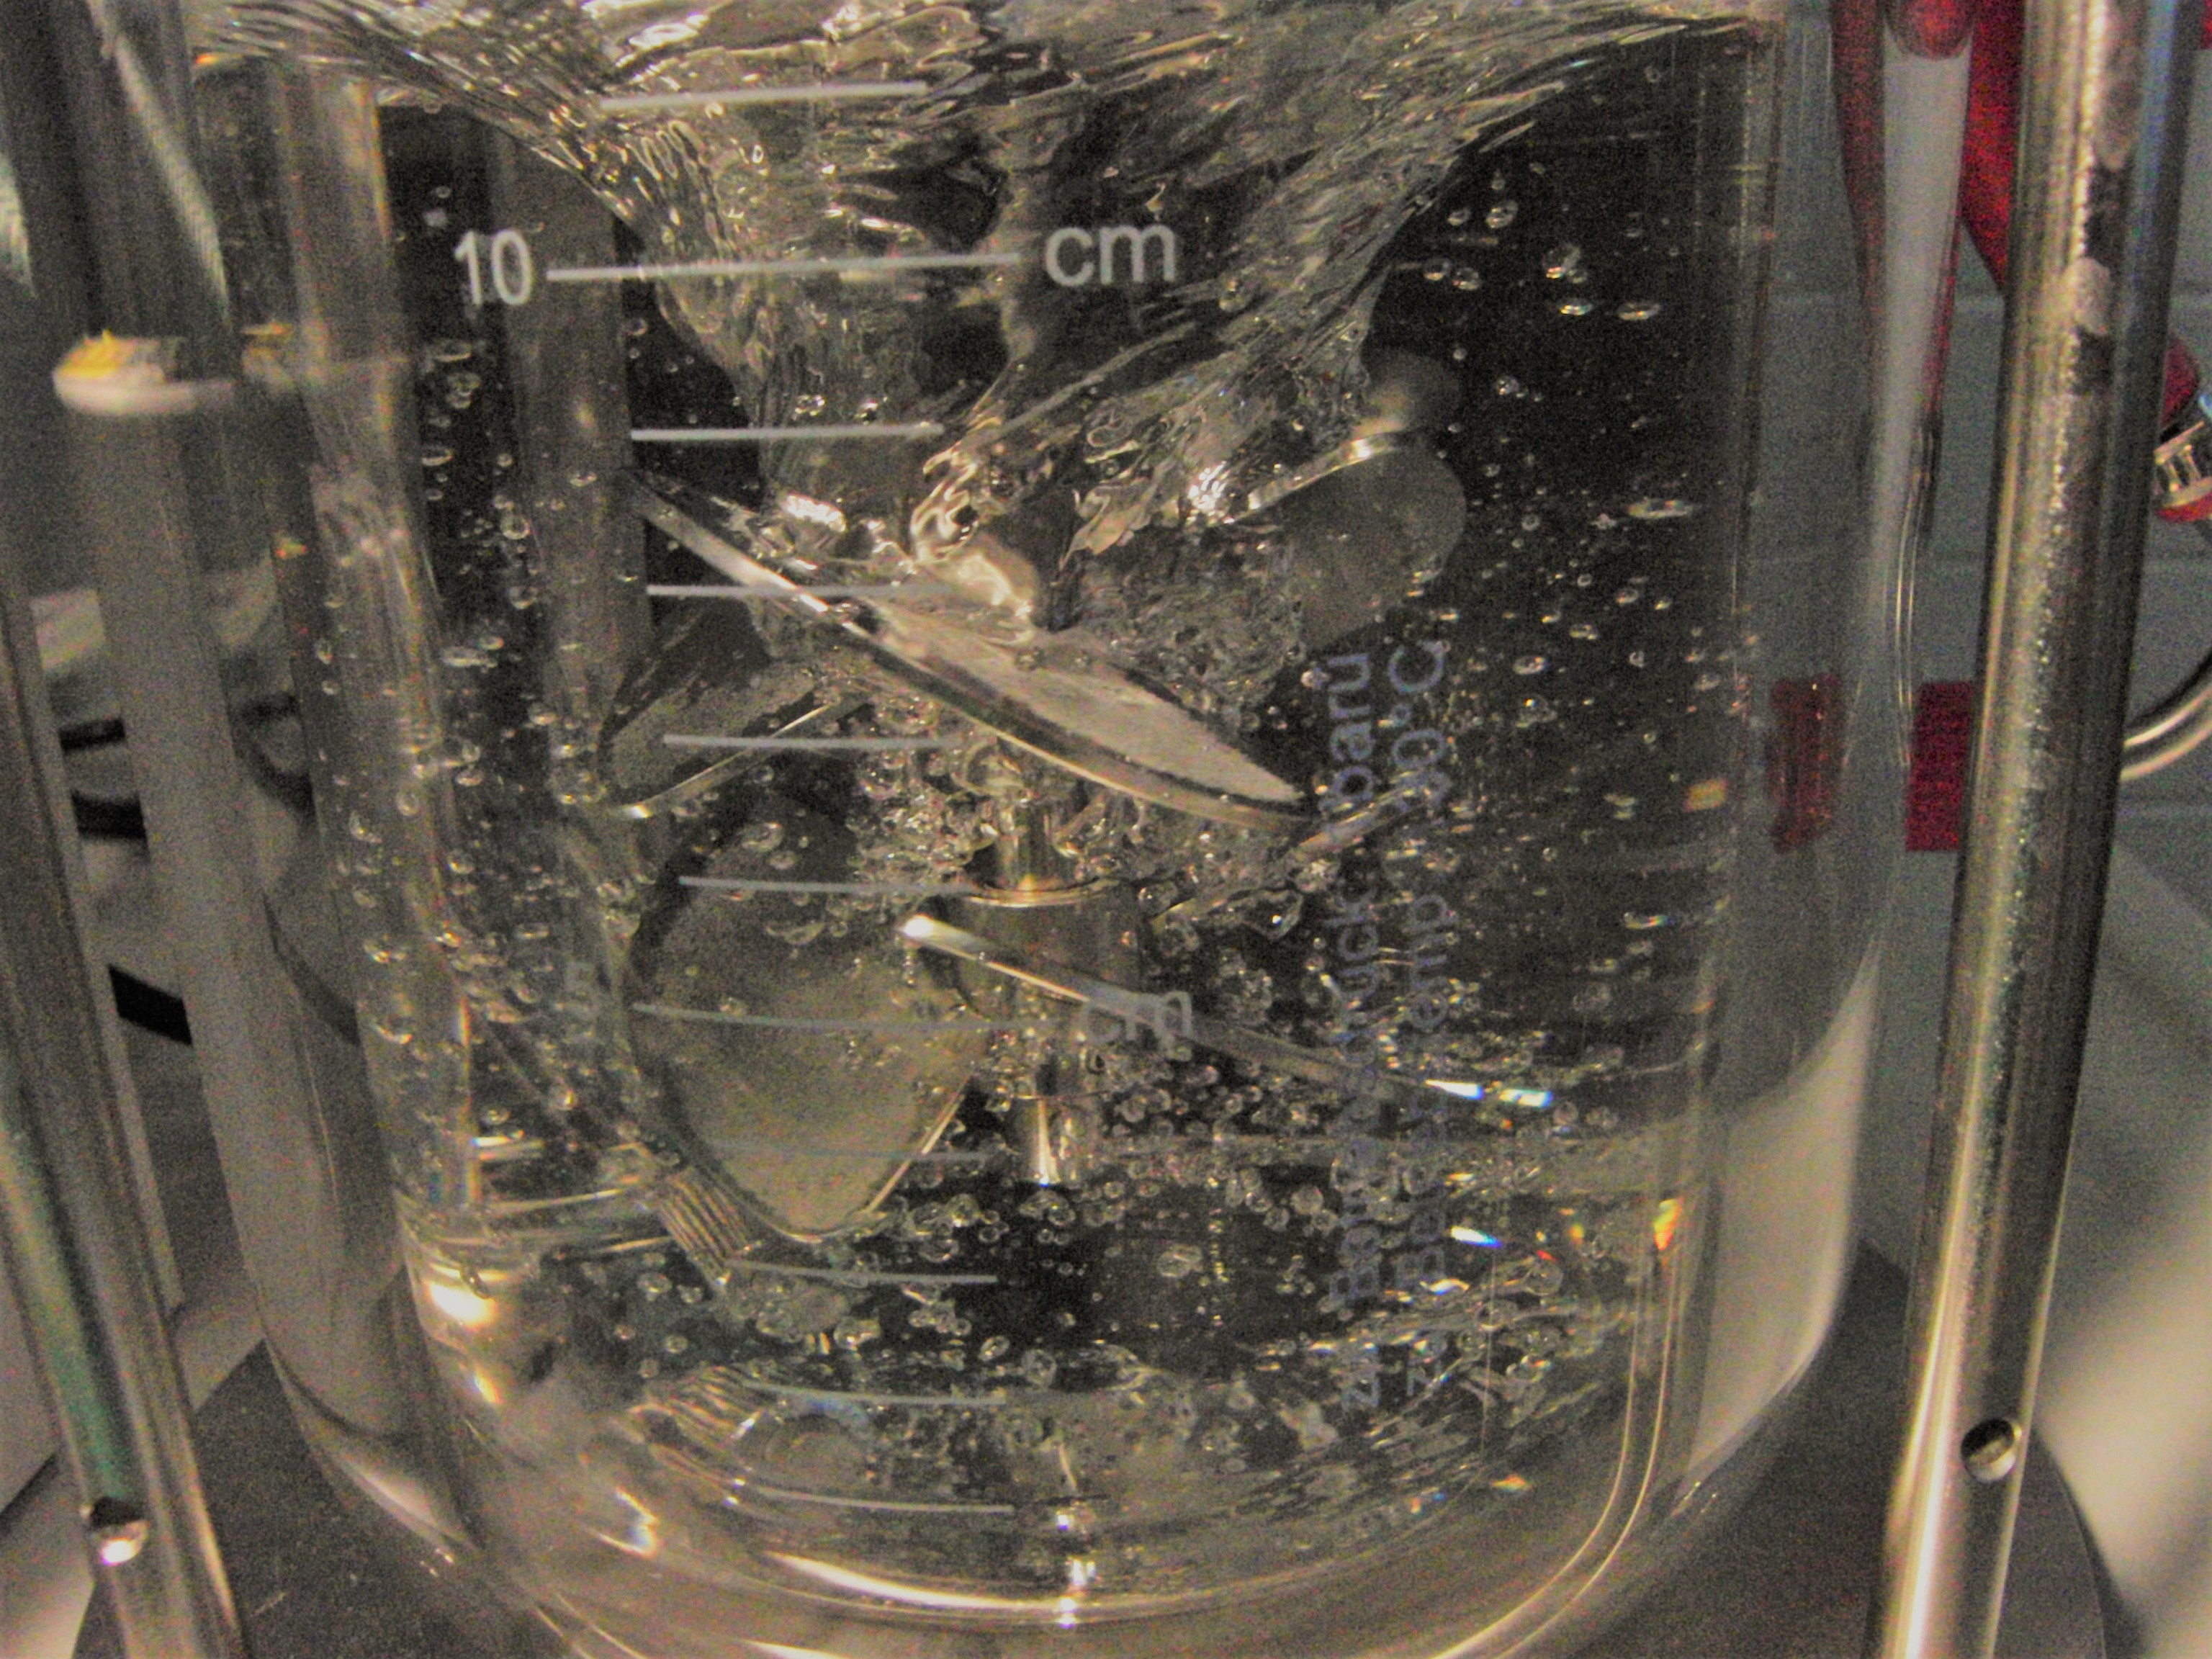
\includegraphics[height=4cm]{Blasenmessung/Versuch_3_2.JPG}}\label{blasengroesse32}
	\hspace{1cm}
	\subfigure[Bild 3]{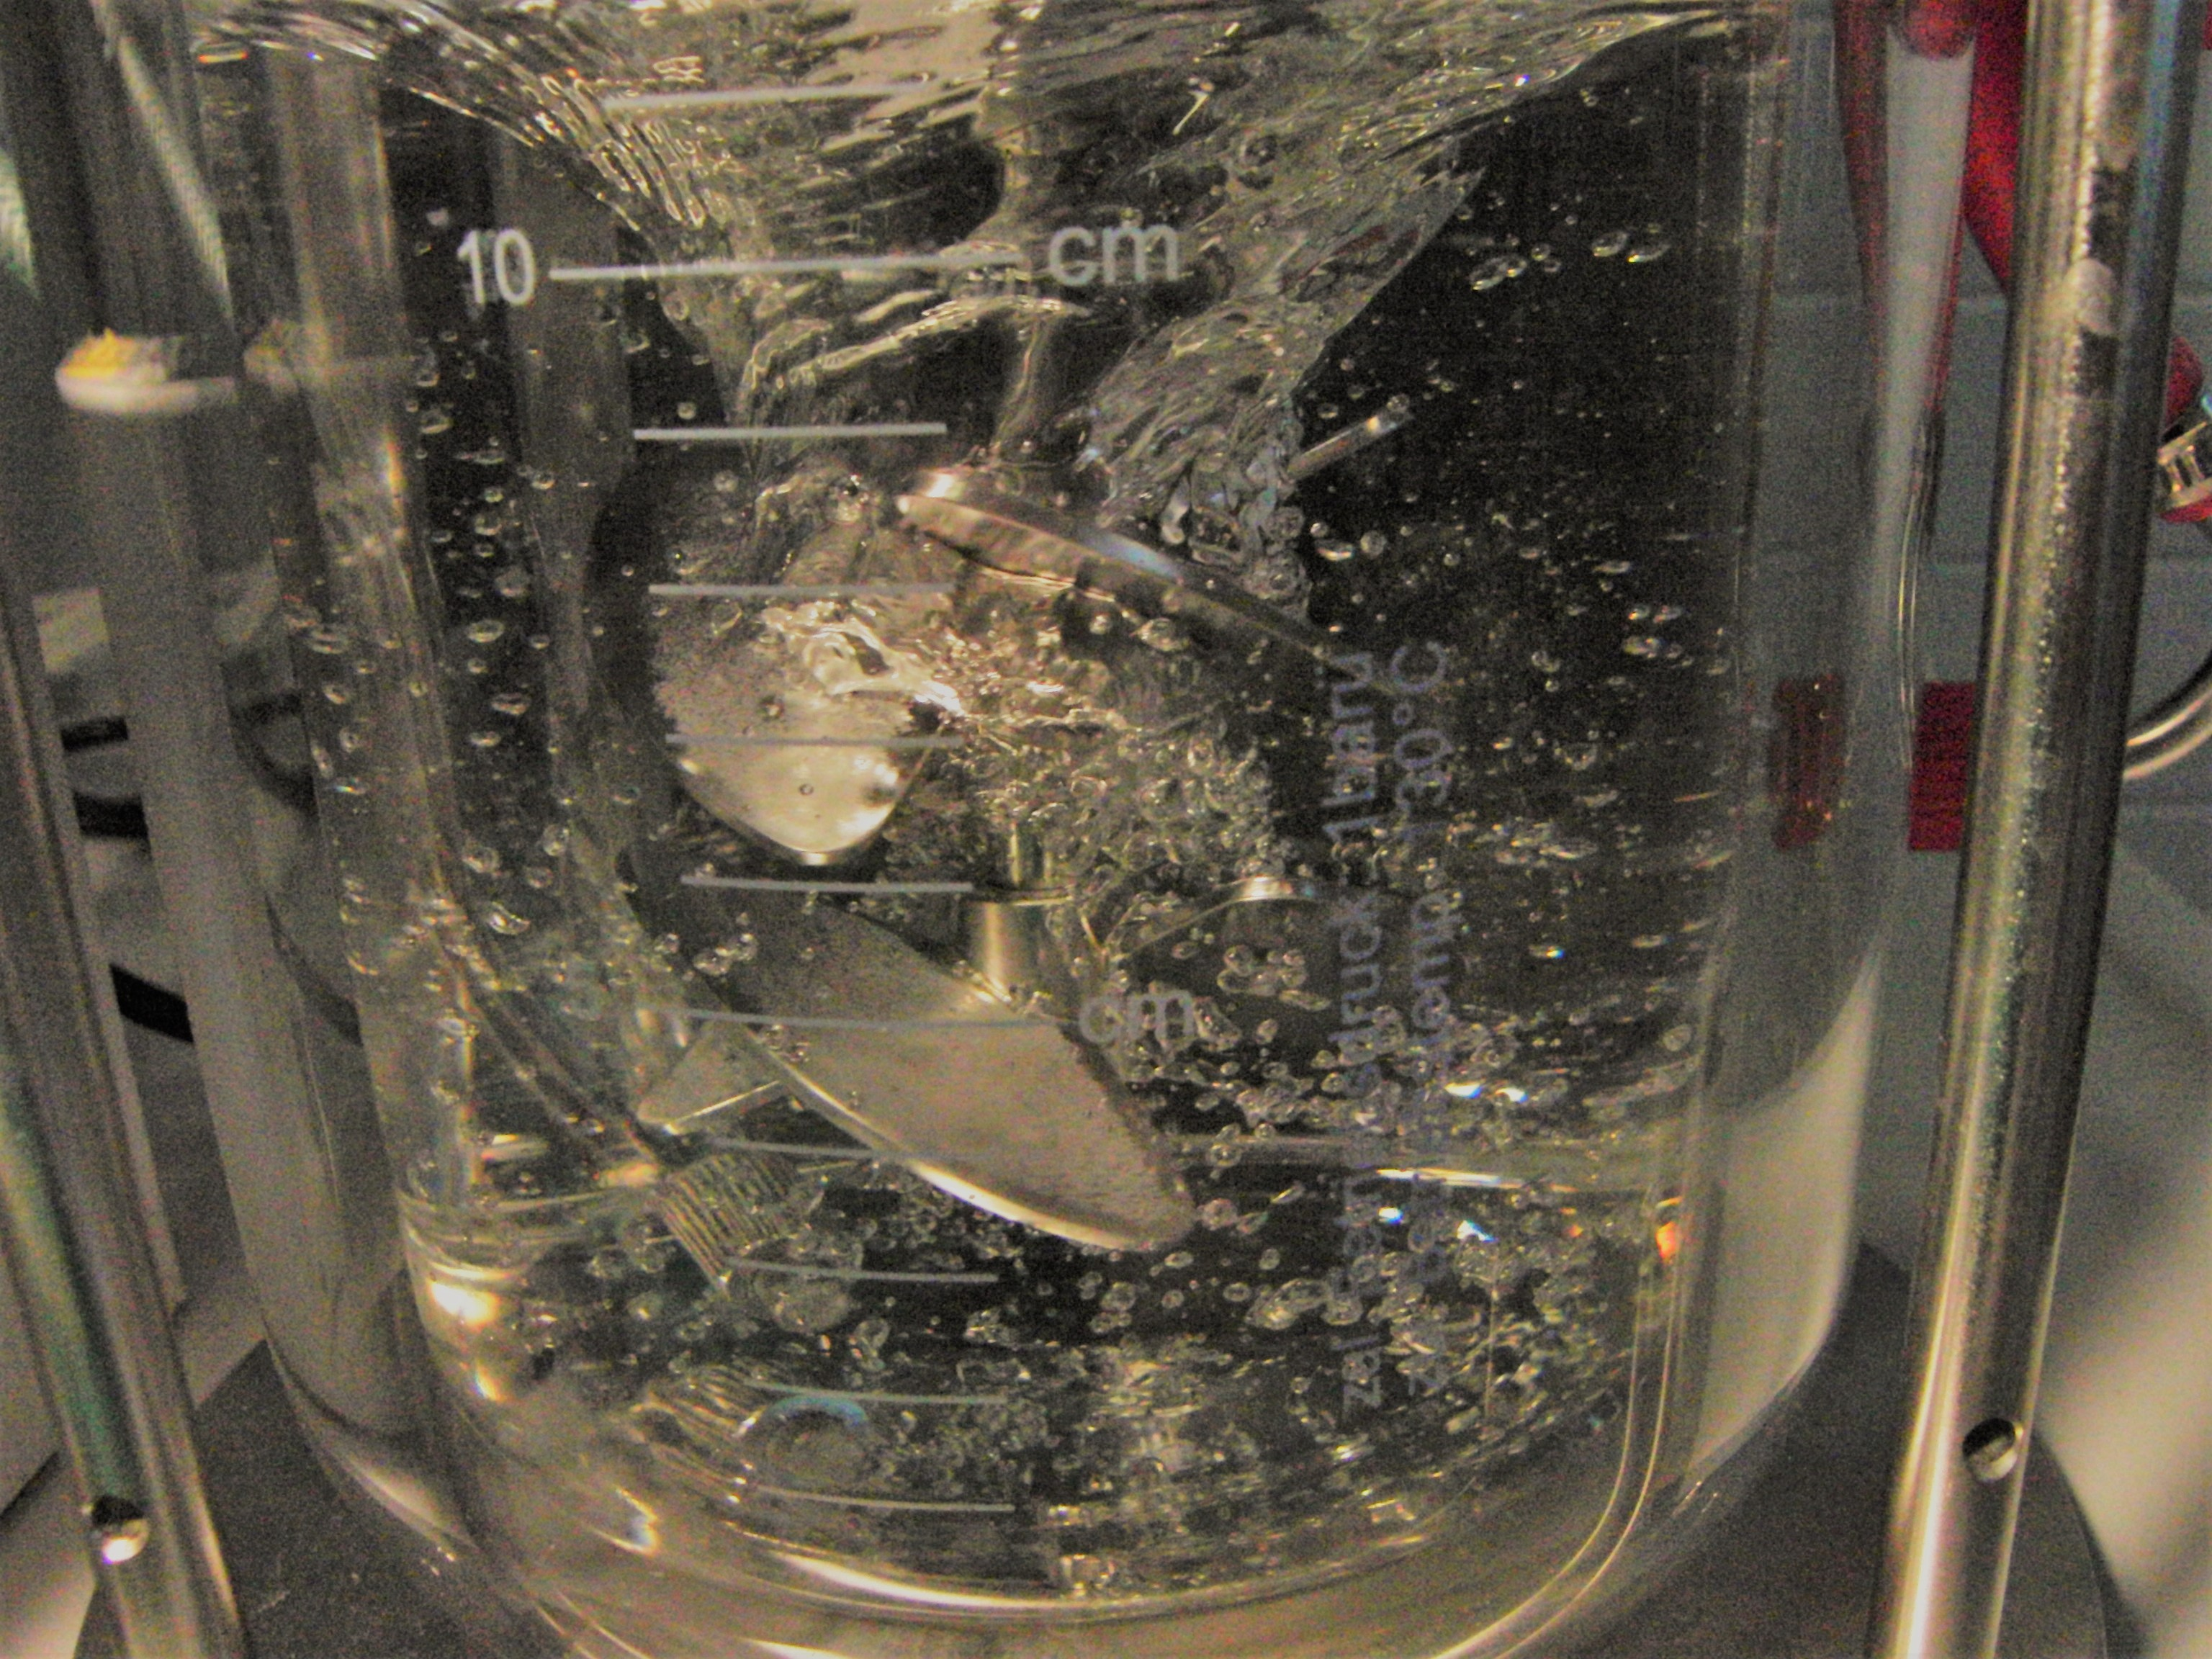
\includegraphics[height=4cm]{Blasenmessung/Versuch_3_3.JPG}}\label{blasengroesse33}
	\hspace{1cm}
	\subfigure[Bild 4]{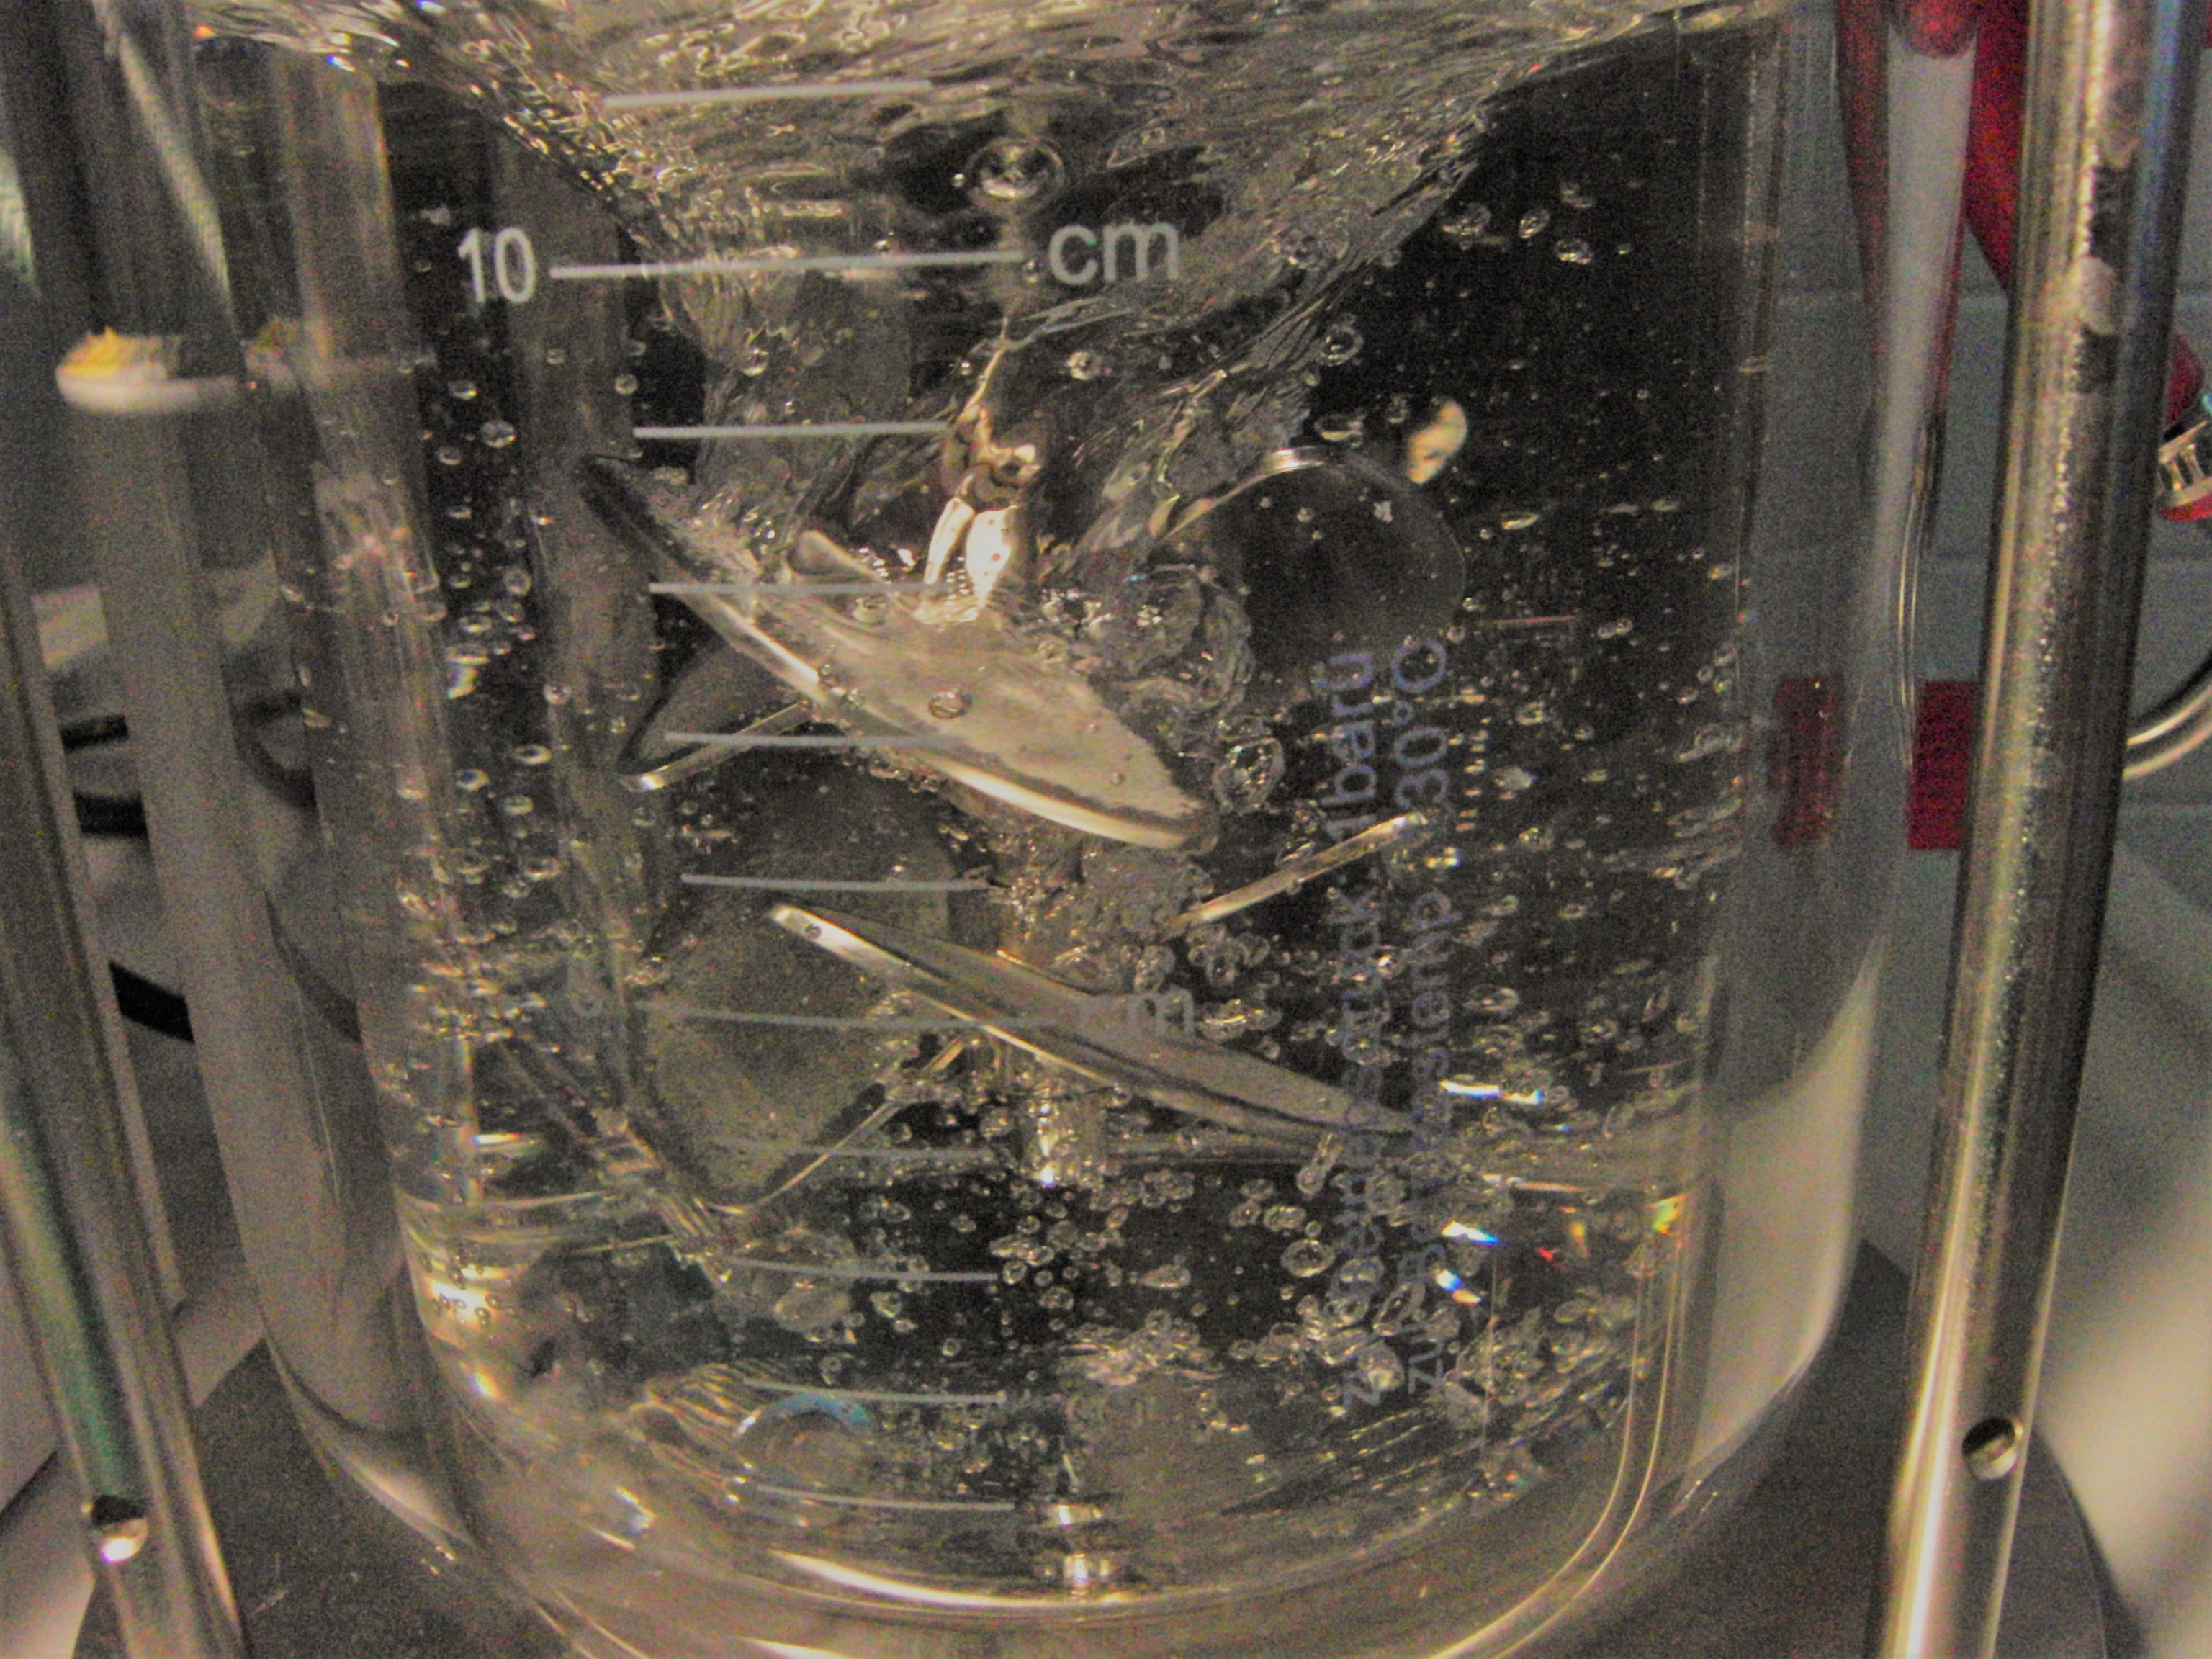
\includegraphics[height=4cm]{Blasenmessung/Versuch_3_4.JPG}}\label{blasengroesse34}
	\hspace{1cm}
	\subfigure[Bild 5]{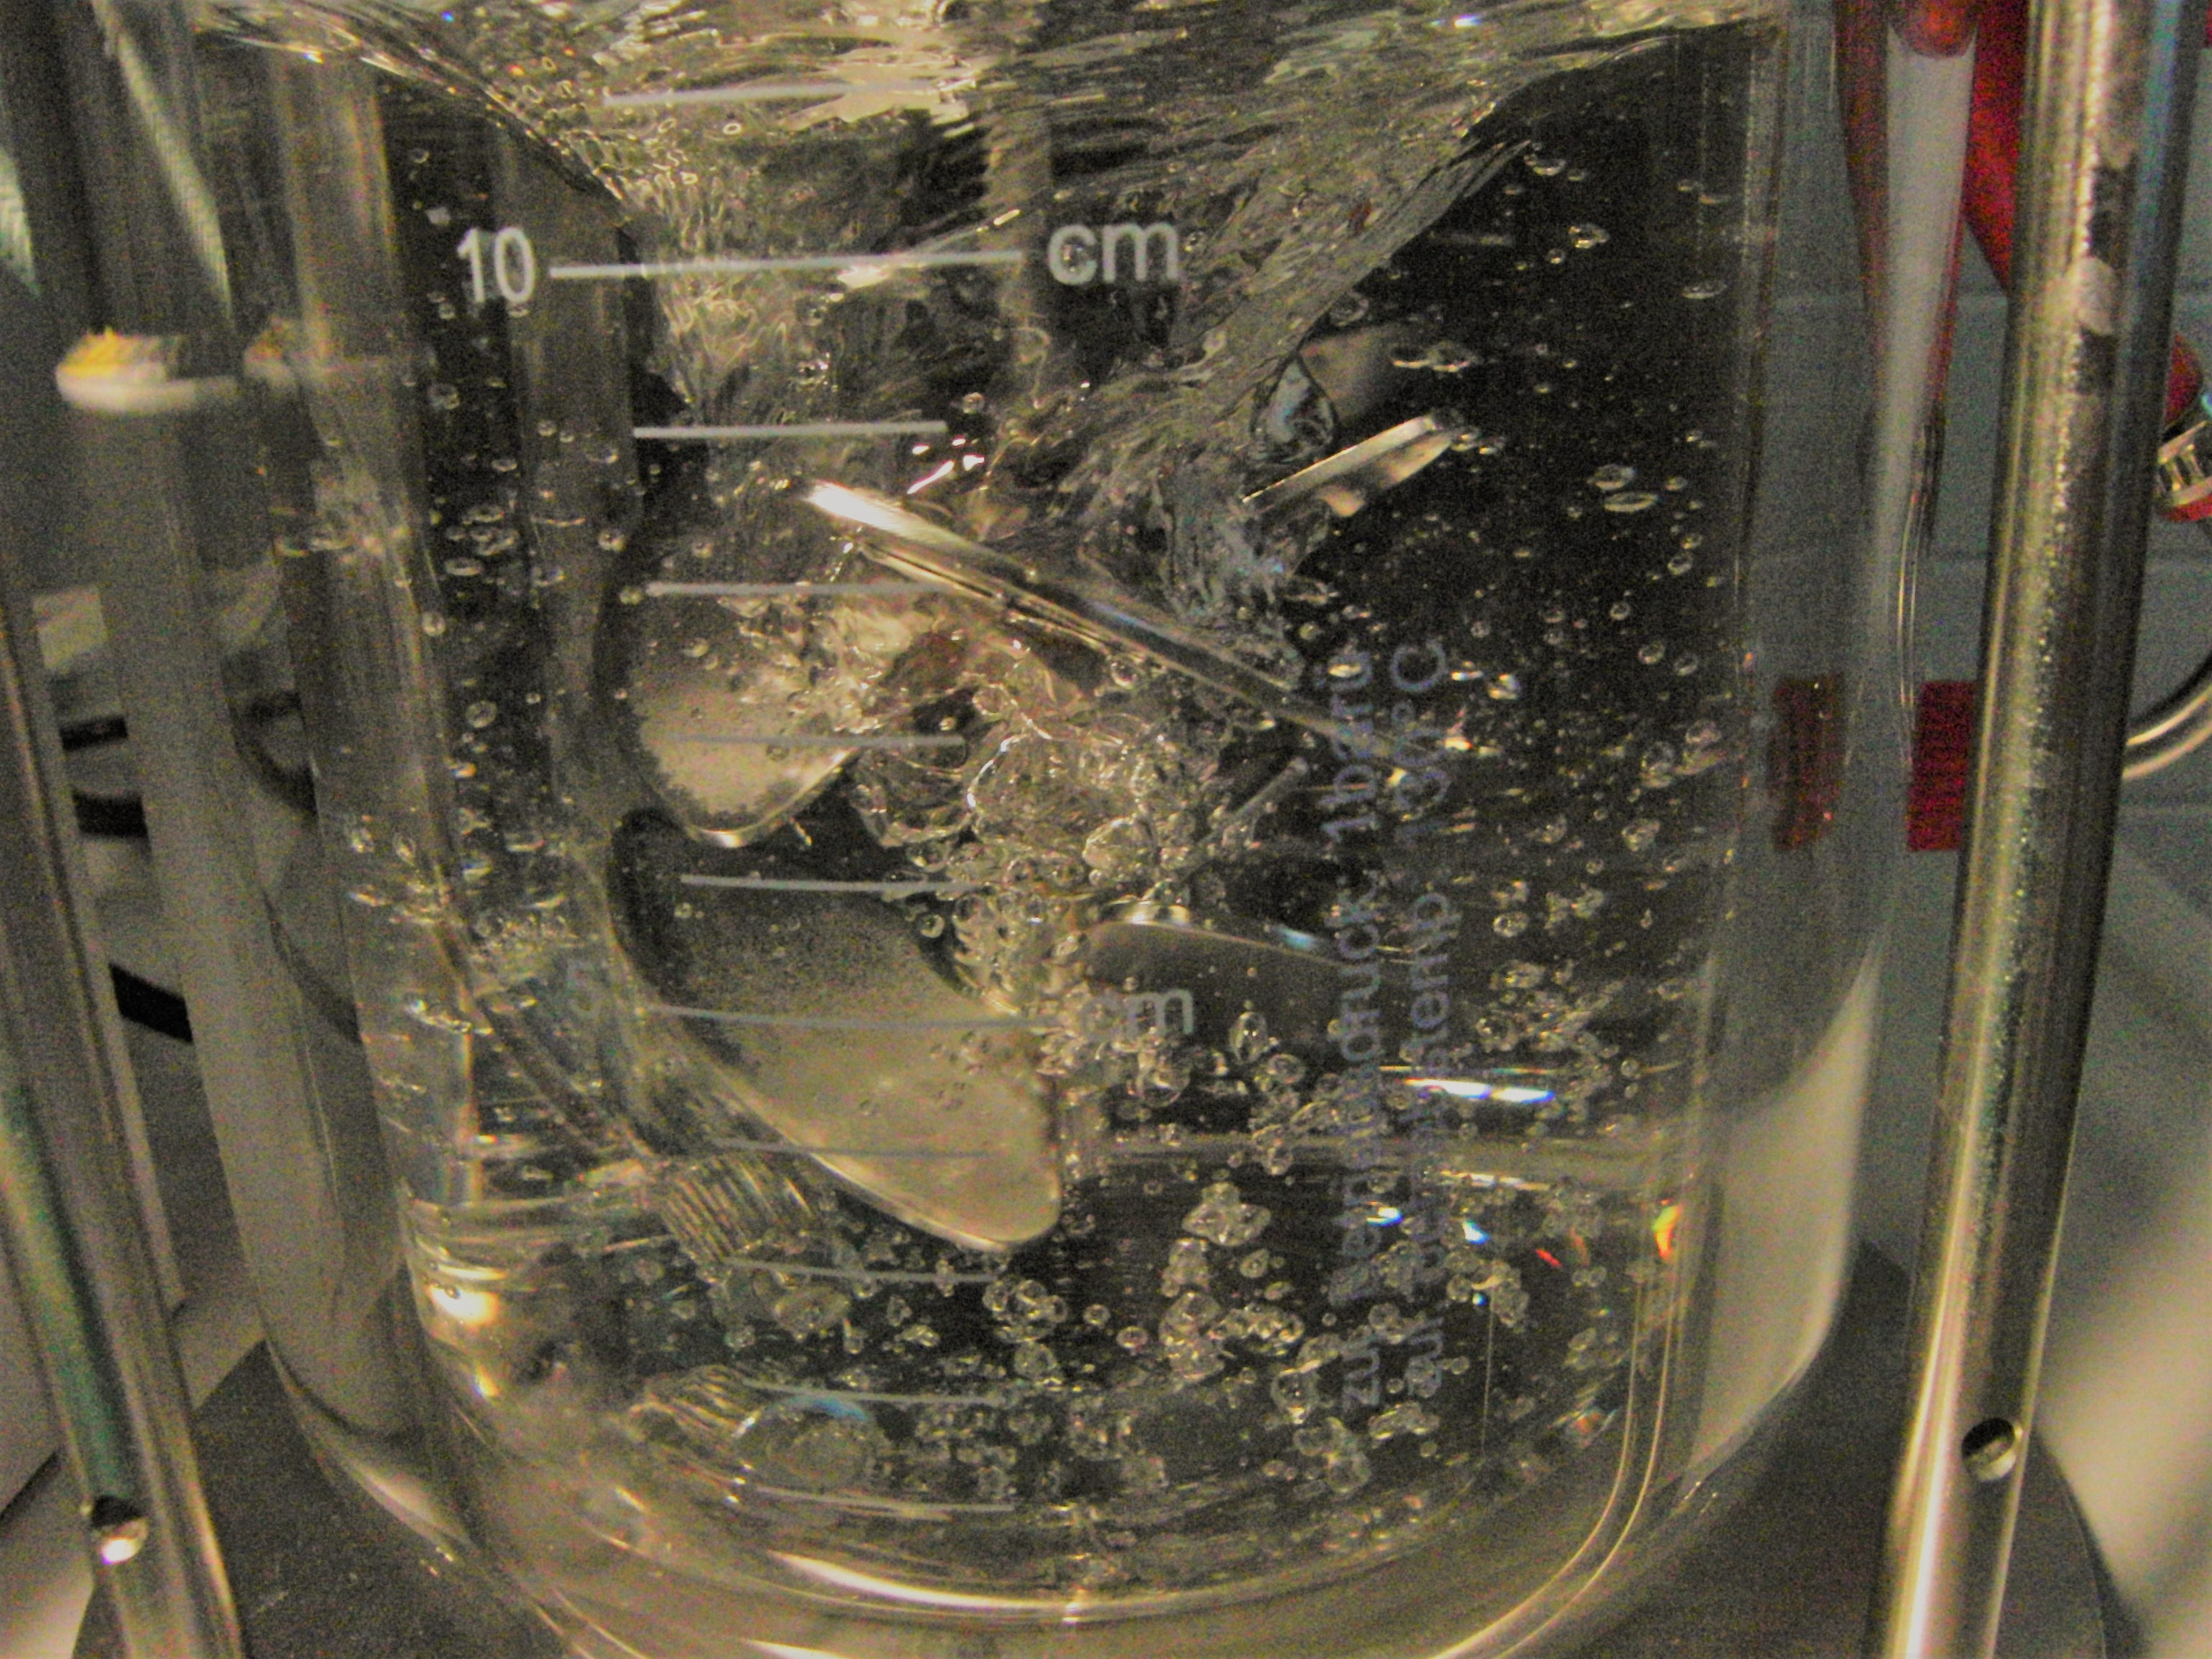
\includegraphics[height=4cm]{Blasenmessung/Versuch_3_5.JPG}}\label{blasengroesse35}
	\hspace{1cm}
	\subfigure[Bild 6]{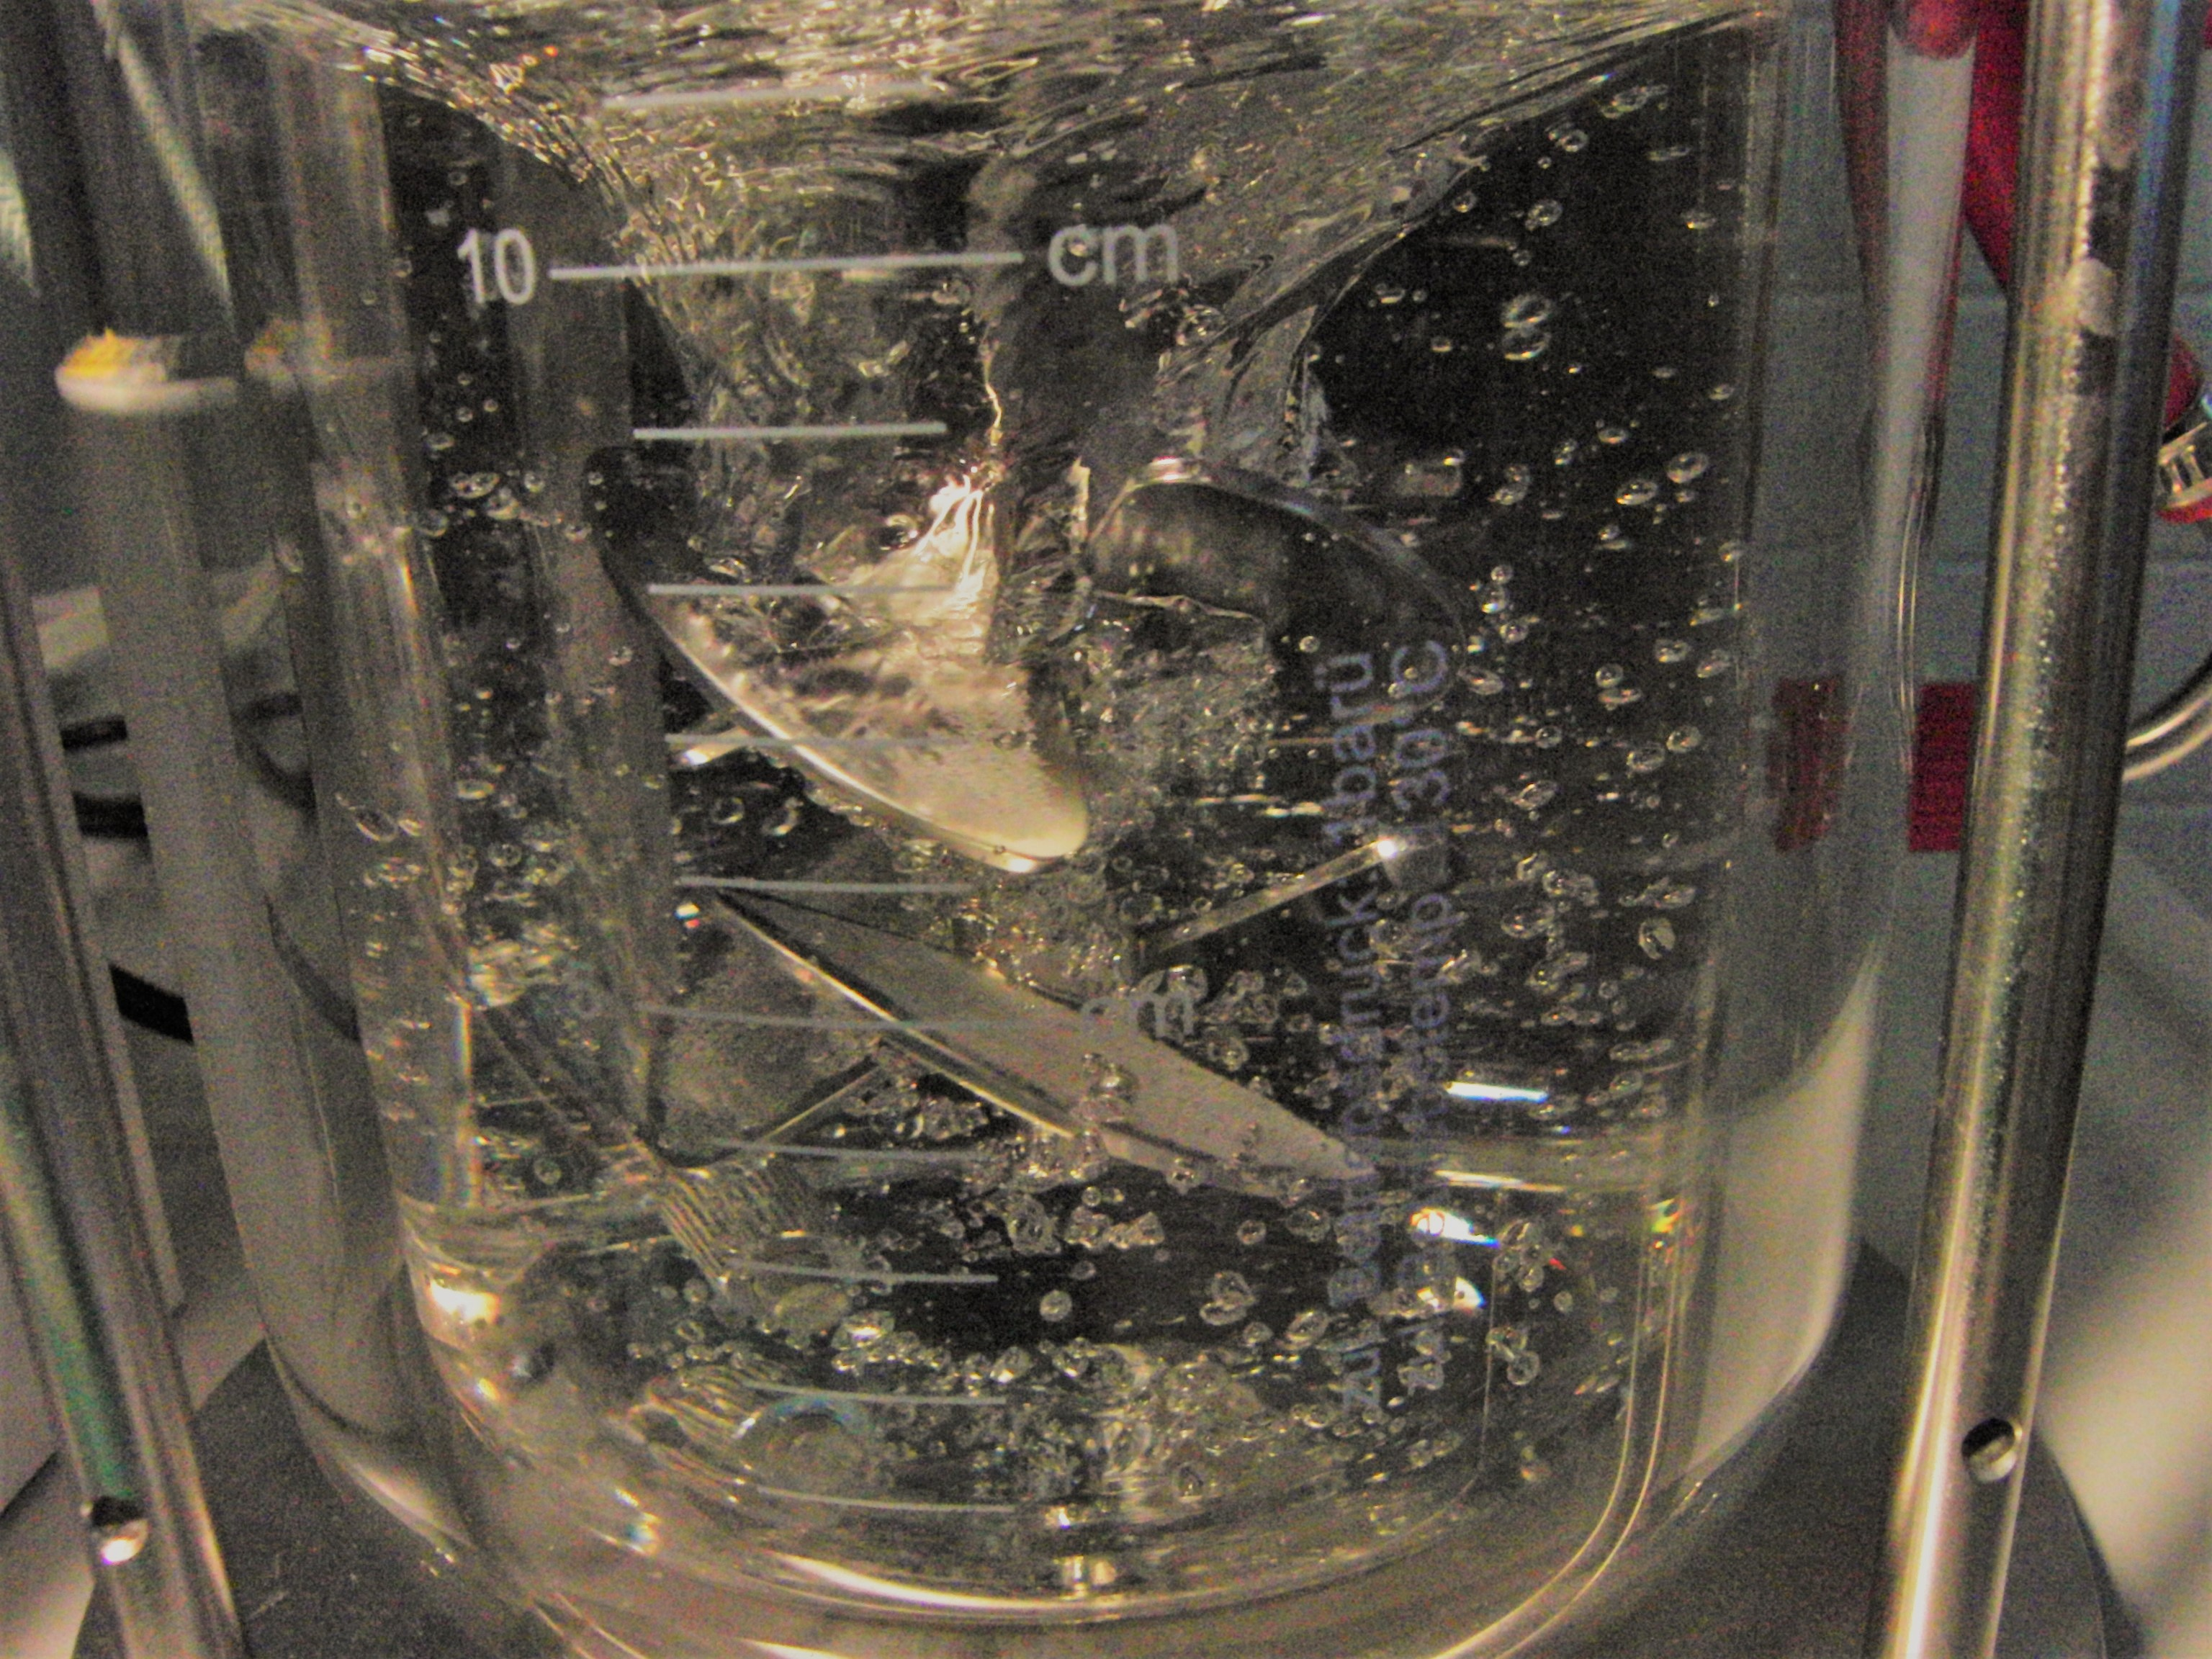
\includegraphics[height=4cm]{Blasenmessung/Versuch_3_6.JPG}}\label{blasengroesse36}
	\caption{Analyse der Blasengröße für Versuch Nr. 3}
	\label{blasengroesseversuch3}
\end{center}	
\end{figure}
\noindent

\begin{table}[H]
  \centering
  \caption{Abgeschätzte Blasenanzahl}
    \begin{tabular}{cccc}
    \toprule
    Bildnummer & Blasenanzahl Reaktor & Mittelwert & Standardabweichung \\
    \midrule
    \multicolumn{4}{c}{Versuch 1}\\
    \midrule
    1&776&\multirow{6}{*}{872}&\multirow{6}{*}{$\pm 58,9$}\\
    2&852&&\\
    3&844&&\\
    4&856&&\\
    5&932&&\\
    6&972&&\\
    \midrule
    \multicolumn{4}{c}{Versuch 2}\\
    \midrule
    1&276&\multirow{8}{*}{268}&\multirow{8}{*}{$\pm 32,7$}\\
    2&296&&\\
    3&252&&\\
    4&208&&\\
    5&316&&\\
    6&224&&\\
    7&284&&\\
    8&288&&\\
    \midrule
    \multicolumn{4}{c}{Versuch 3}\\
    \midrule
    1&656&\multirow{6}{*}{670}&\multirow{6}{*}{$\pm 34,5$}\\
    2&664&&\\
    3&684&&\\
    4&644&&\\
    5&744&&\\
    6&628&&\\   
    \bottomrule
    \end{tabular}
  \label{tab:Blasenanzahl}
\end{table}

\begin{table}[H]
	\centering
	\caption{Abgeschätzter Blasendurchmesser}
	\begin{tabular}{cccc}
		\toprule
		Bildnummer & Blasendurchmesser Reaktor in mm& Mittelwert & Standardabweichung \\
		\midrule
		\multicolumn{4}{c}{Versuch 1}\\
		\midrule
		1&1,8&\multirow{6}{*}{2,0}&\multirow{6}{*}{$\pm 0,18$}\\
		2&1,8&&\\
		3&1,9&&\\
		4&1,8&&\\
		5&2,2&&\\
		6&2,3&&\\
		\midrule
		\multicolumn{4}{c}{Versuch 2}\\
		\midrule
		1&3,6&\multirow{8}{*}{3,7}&\multirow{8}{*}{$\pm 0,33$}\\
		2&4,5&&\\
		3&3,5&&\\
		4&3,5&&\\
		5&3,5&&\\
		6&3,6&&\\
		7&4,0&&\\
		8&3,5&&\\
		\midrule
		\multicolumn{4}{c}{Versuch 3}\\
		\midrule
		1&1,2&\multirow{6}{*}{1,3}&\multirow{6}{*}{$\pm 0,08$}\\
		2&1,3&&\\
		3&1,2&&\\
		4&1,4&&\\
		5&1,3&&\\
		6&1,4&&\\   
		\bottomrule
	\end{tabular}
	\label{tab:Blasendurchmesser}
\end{table}

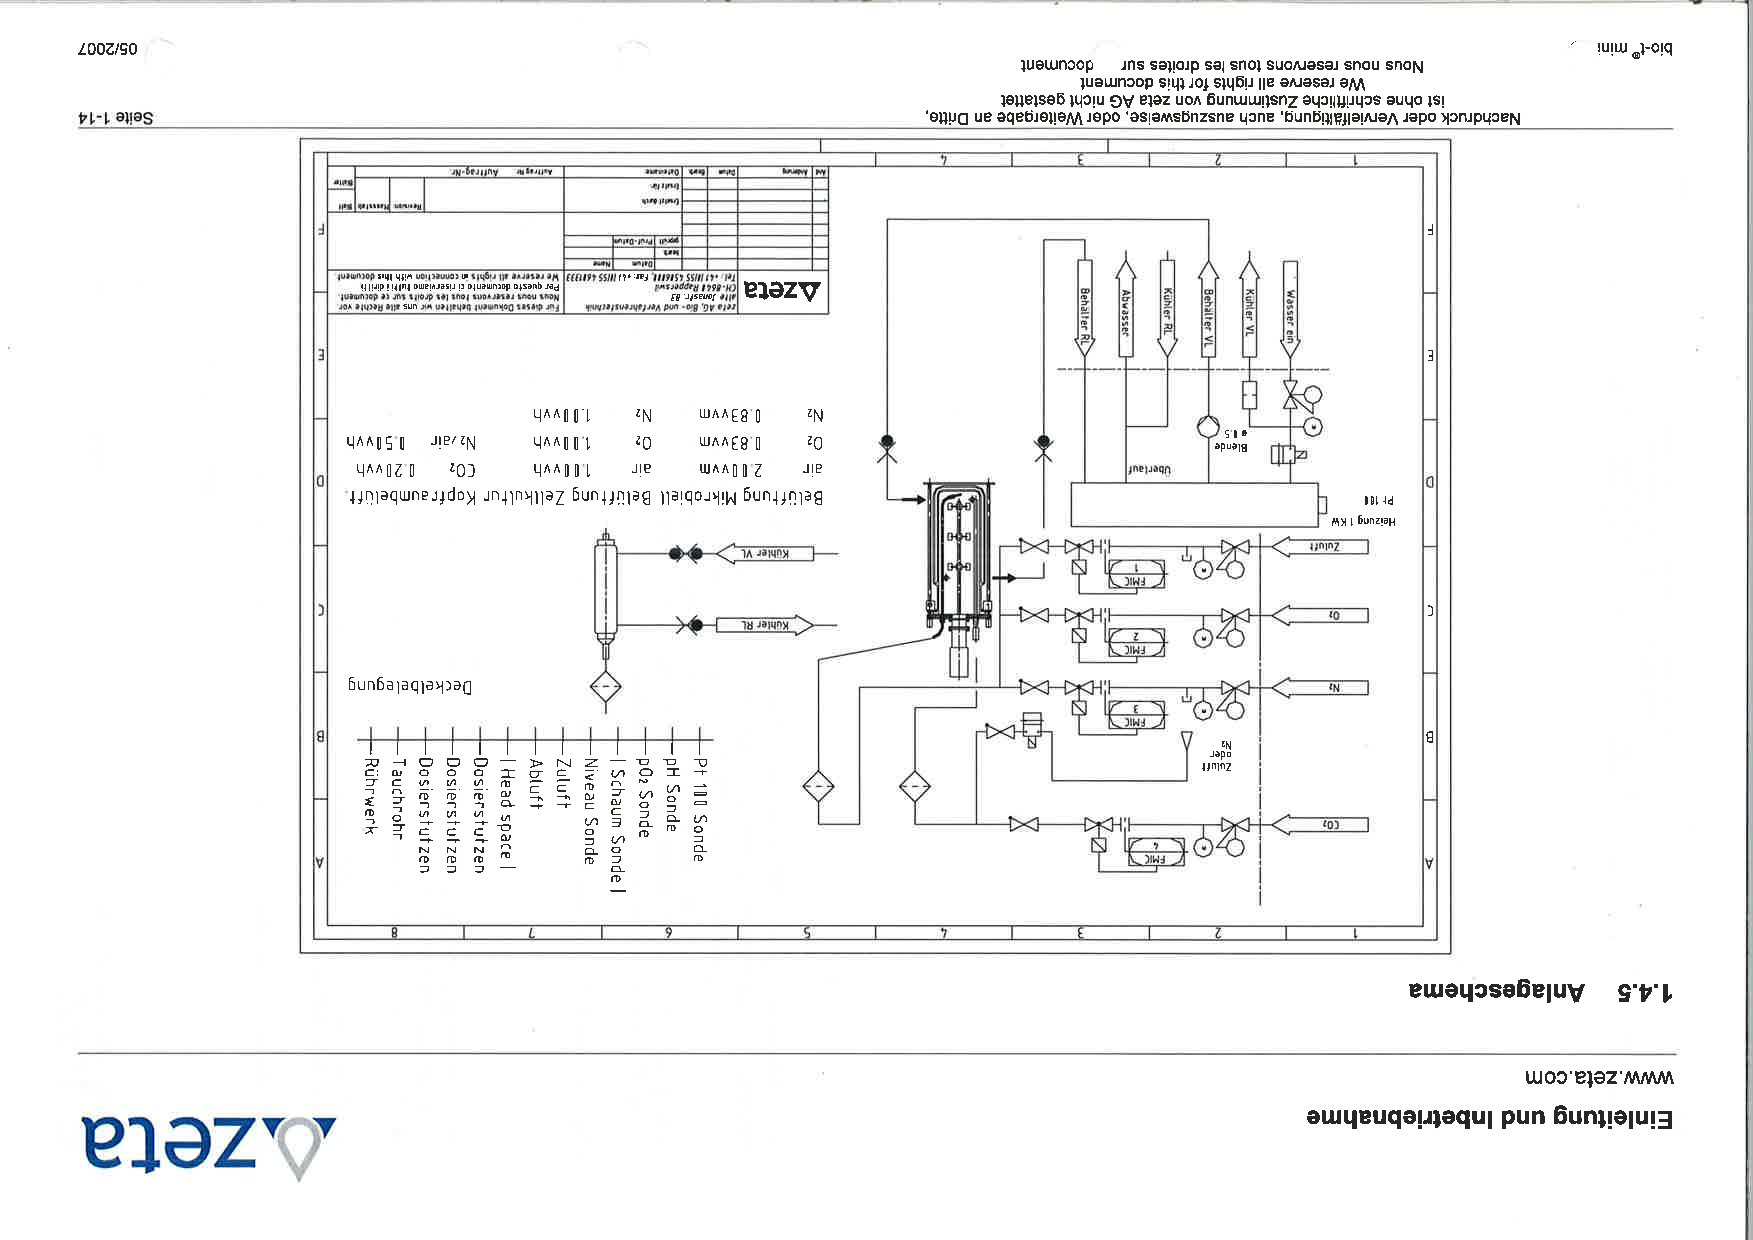
\includepdf[angle=90,pages=1]{anlageschema} \newpage
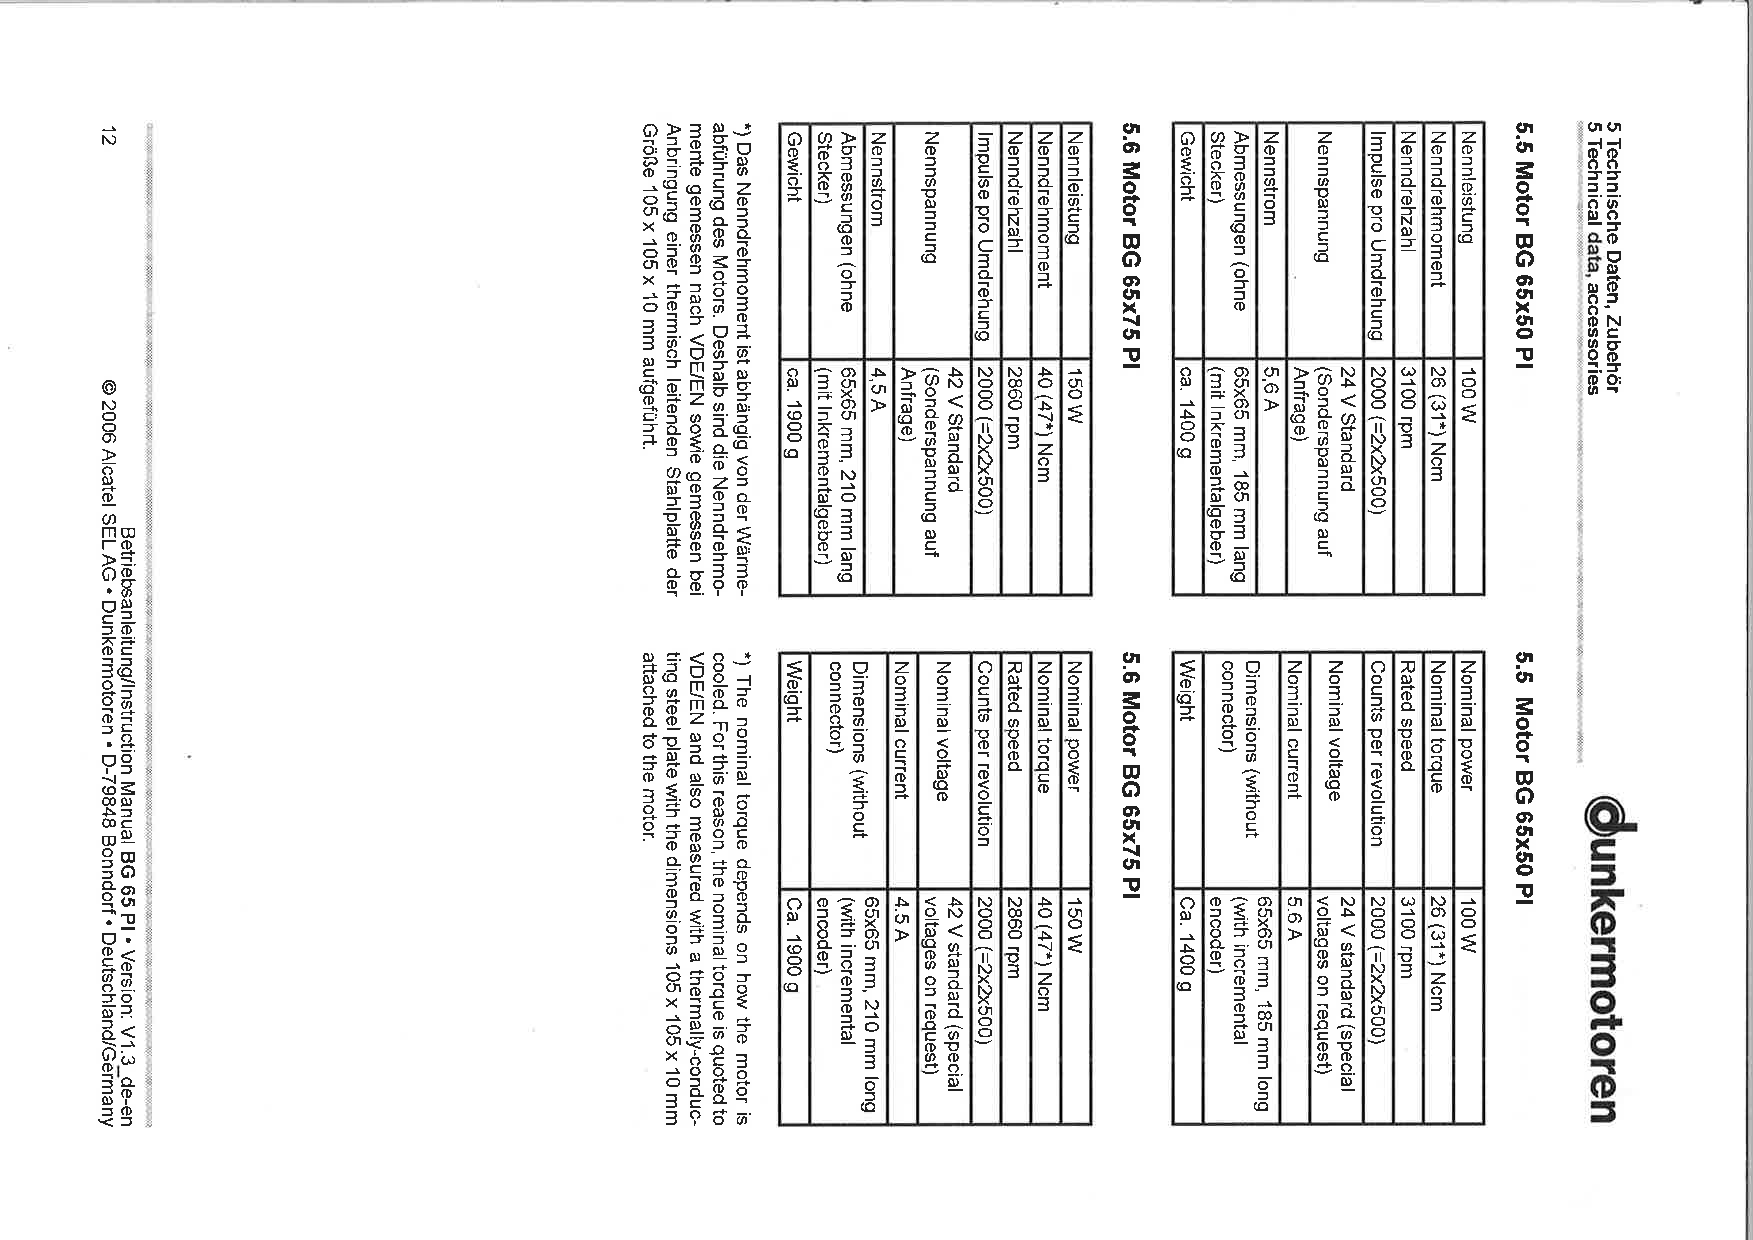
\includepdf[angle=90,pages=1]{motor} \newpage
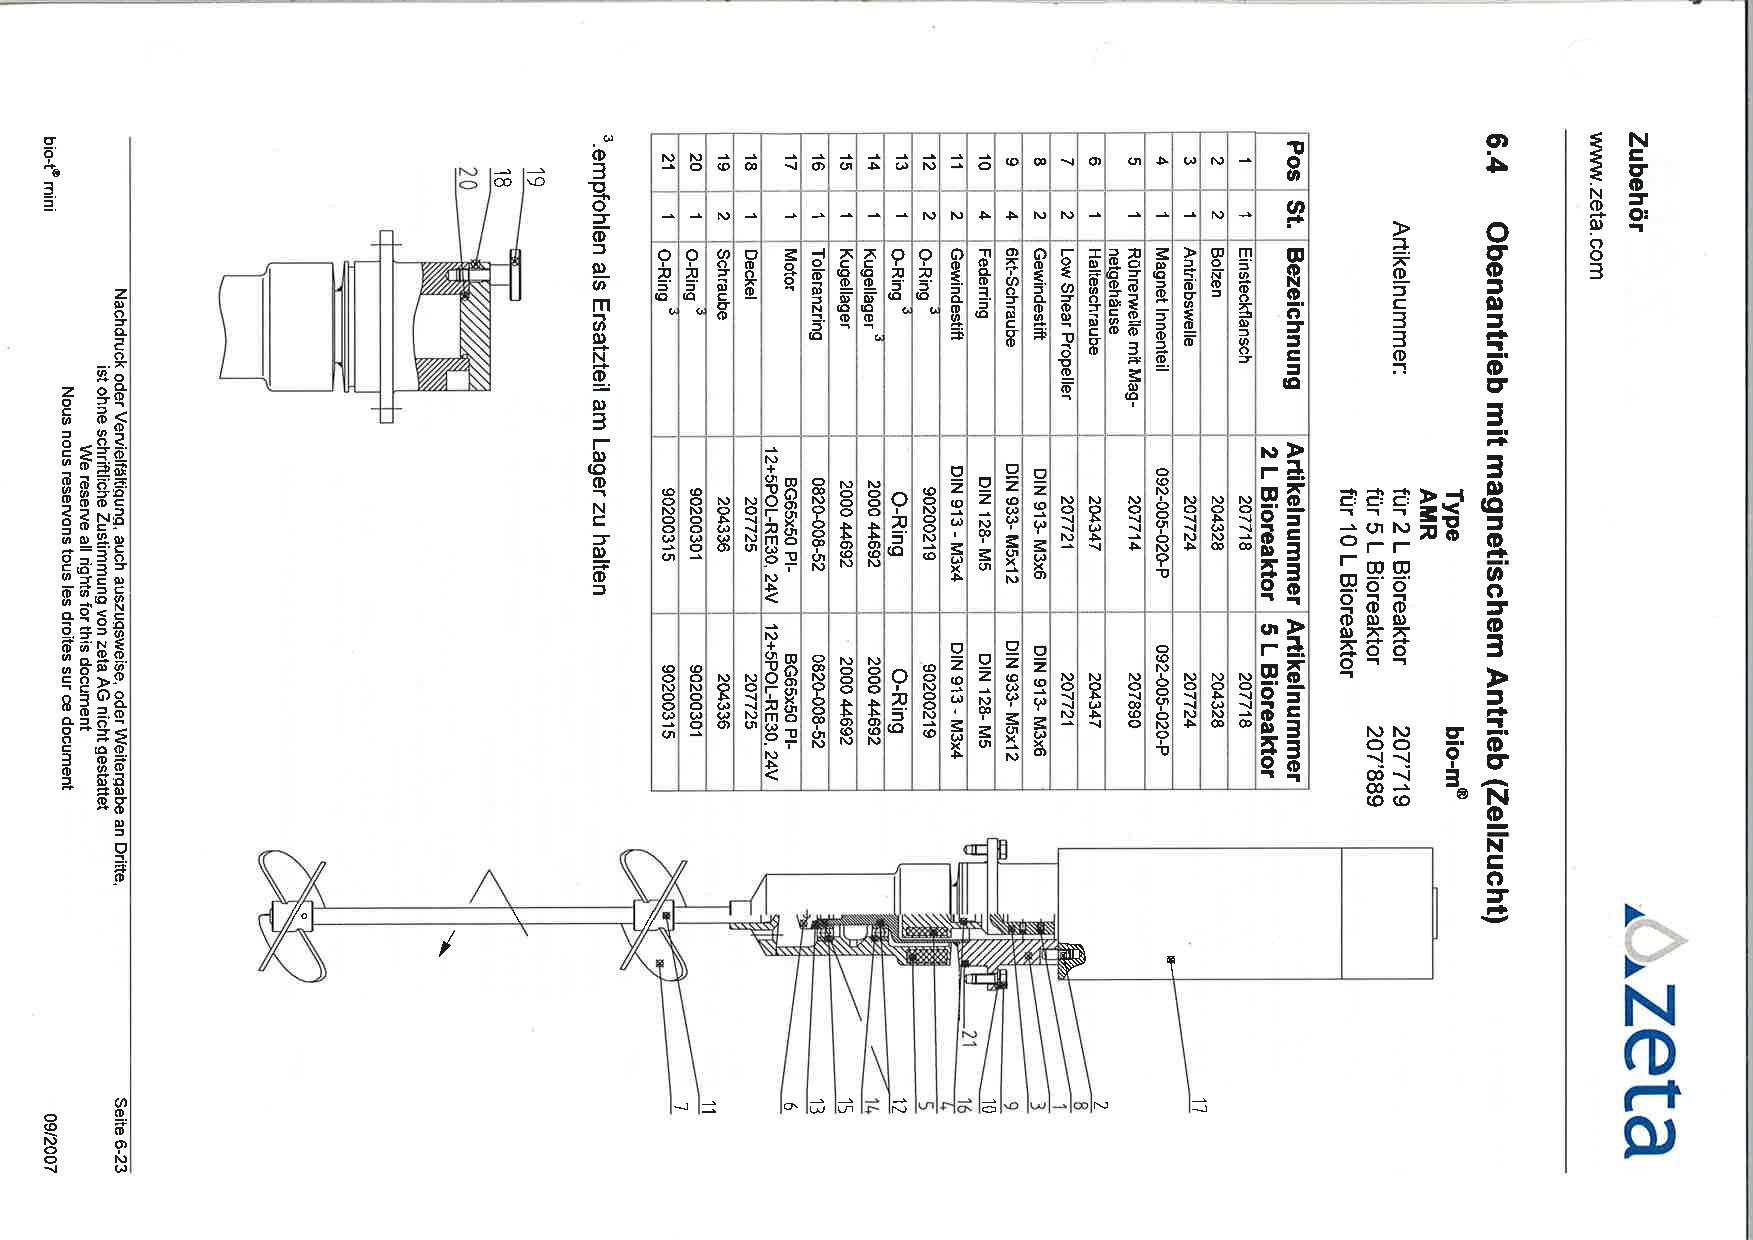
\includepdf[angle=90,pages=1]{obnantrieb-bauteiliste} \newpage
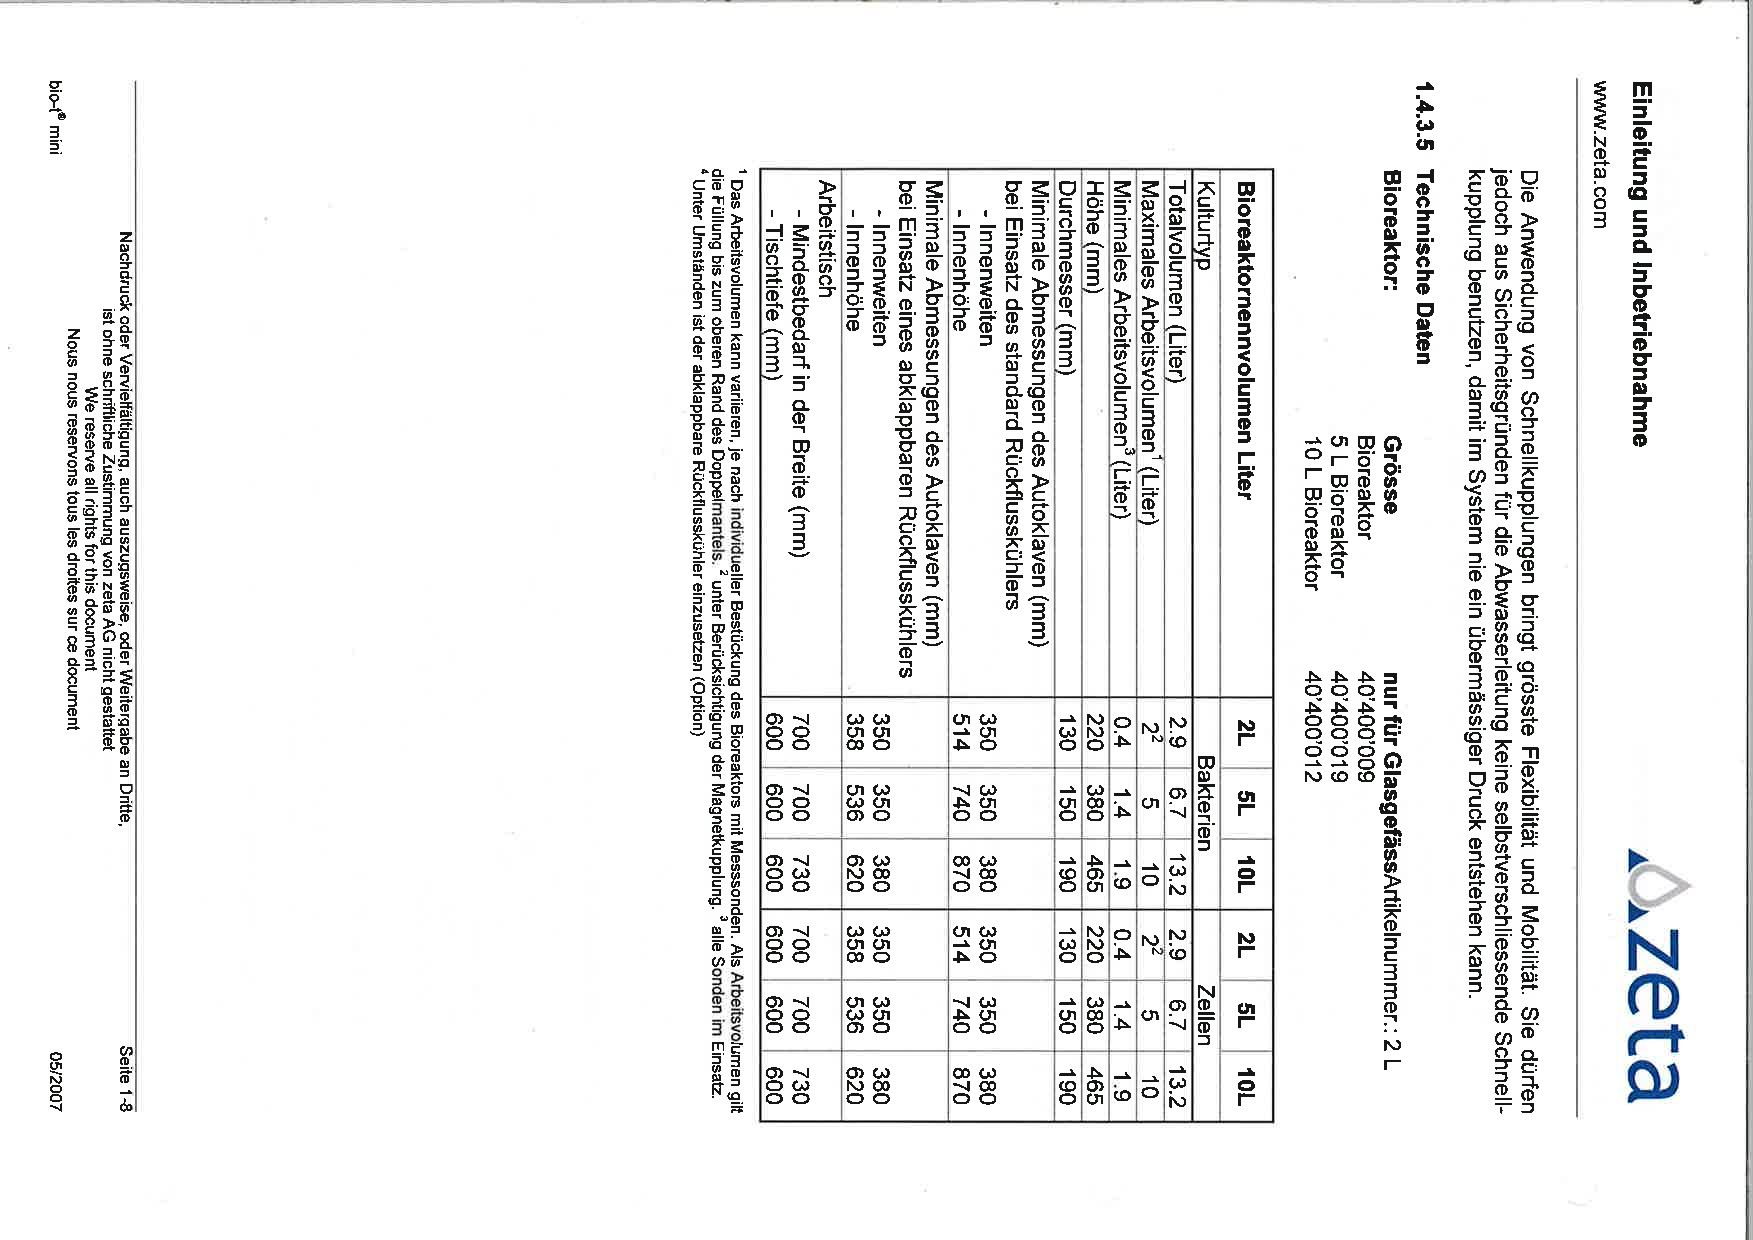
\includepdf[angle=90,pages=1]{spez_reak1} \newpage
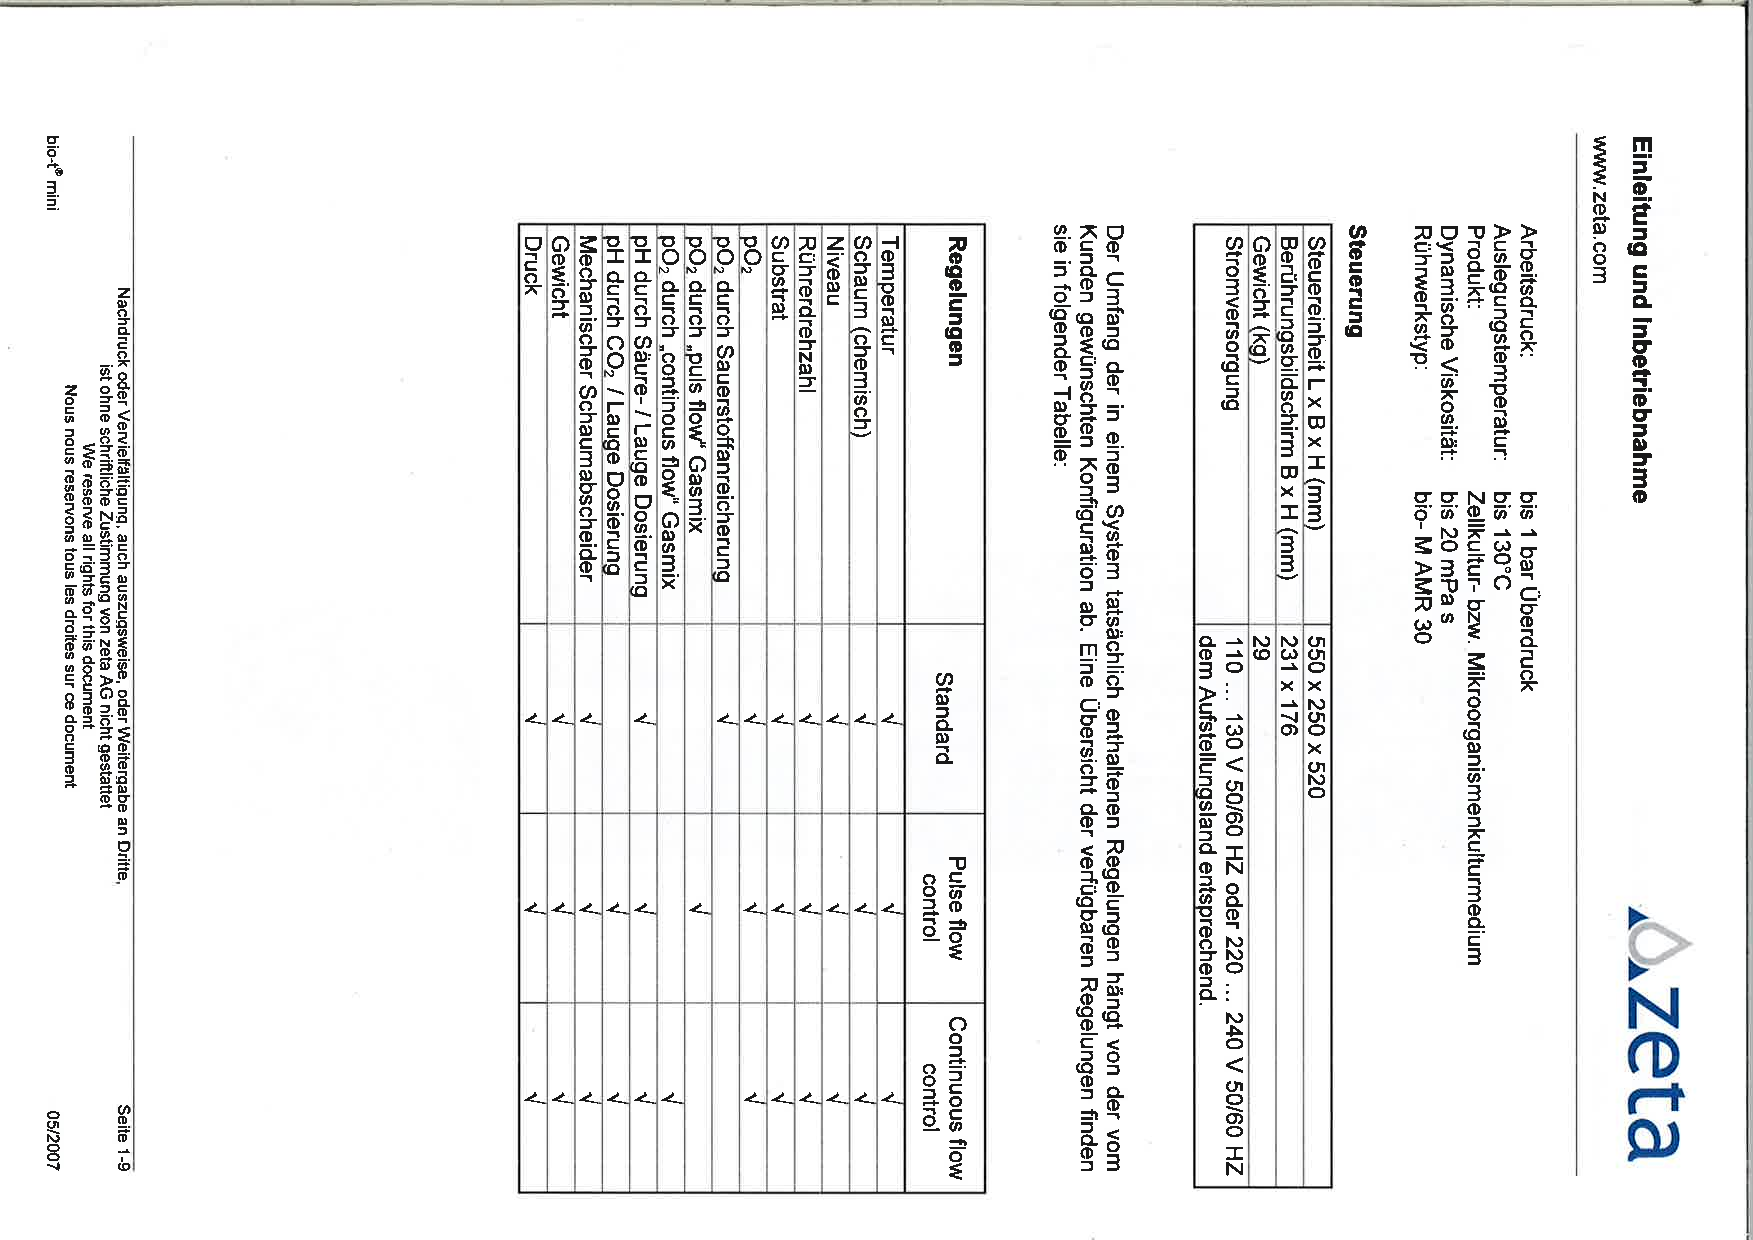
\includepdf[angle=90,pages=1]{spez_reak2} \newpage
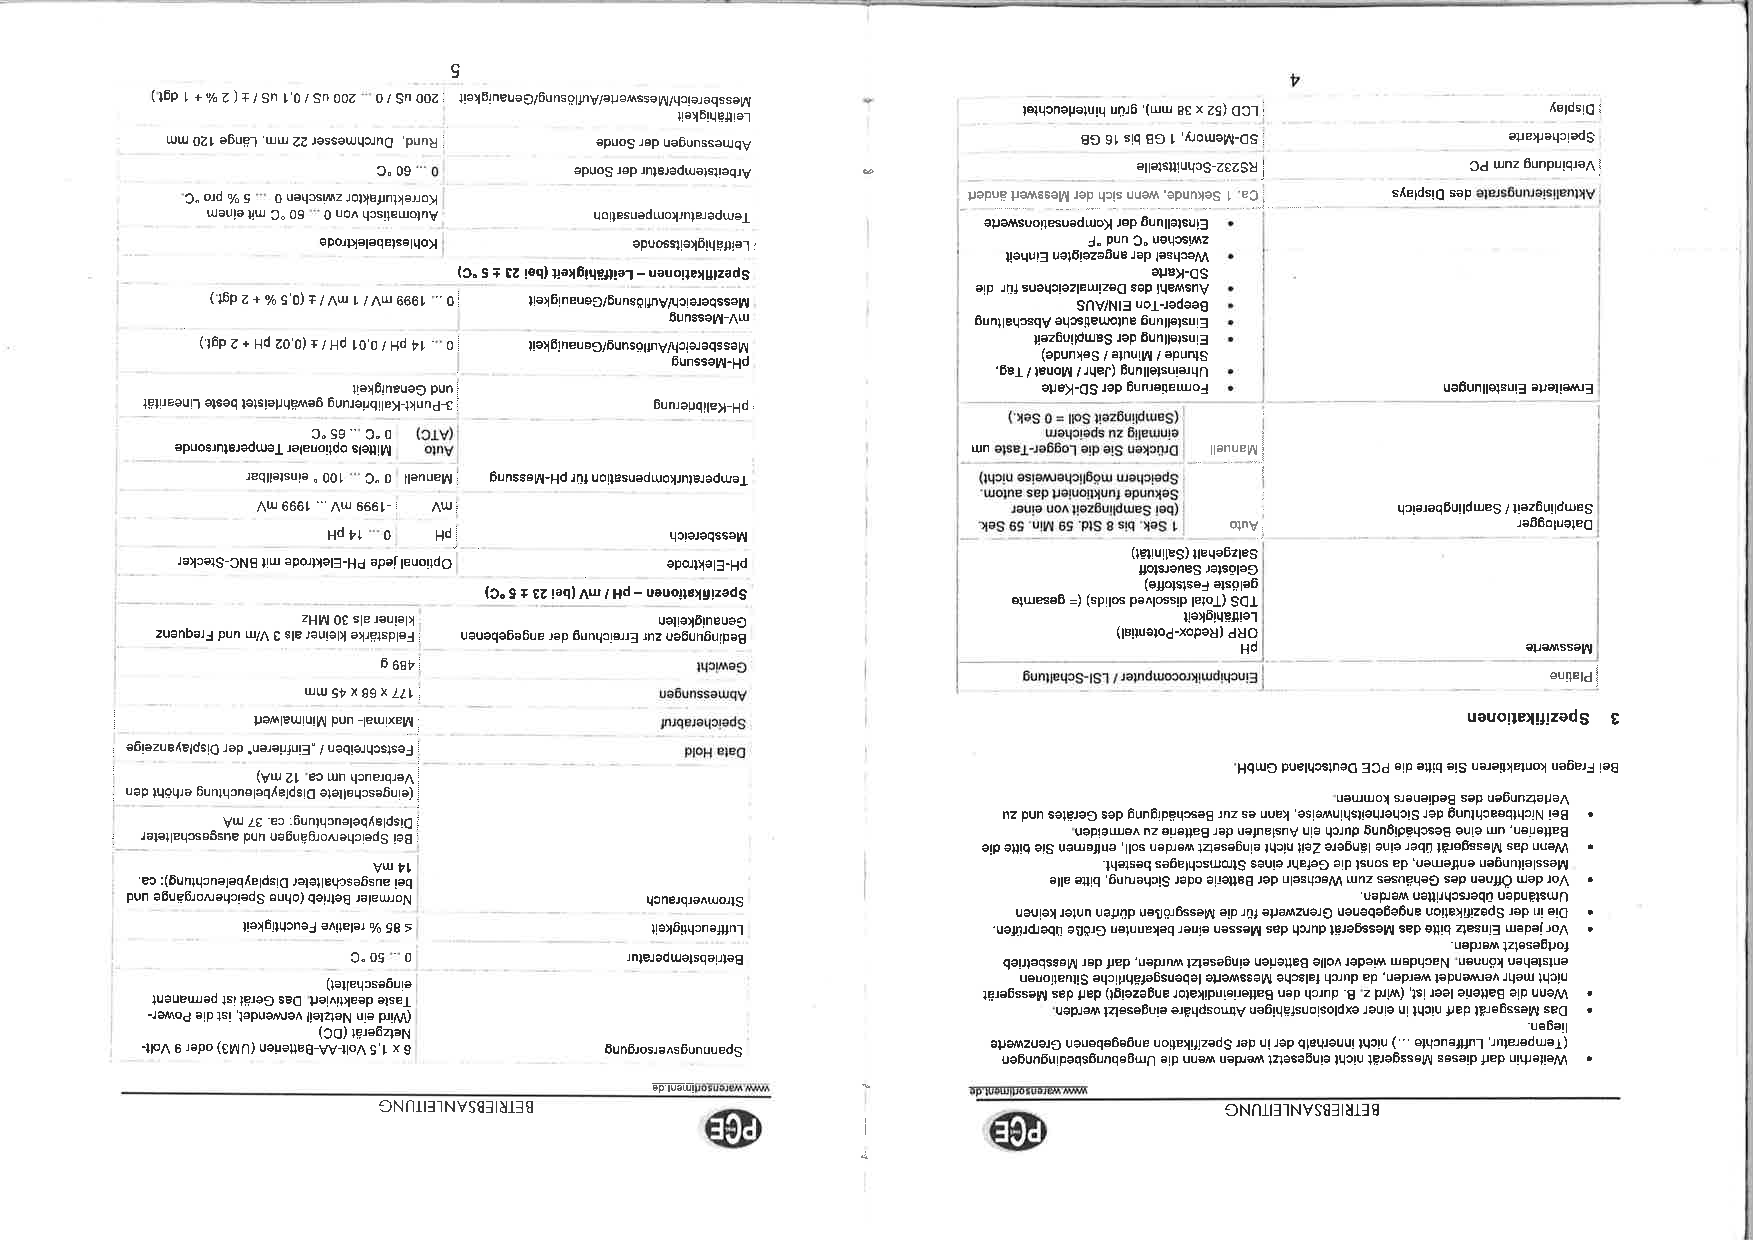
\includepdf[angle=180,pages=1]{spez-sauerstoffmesser} \newpage
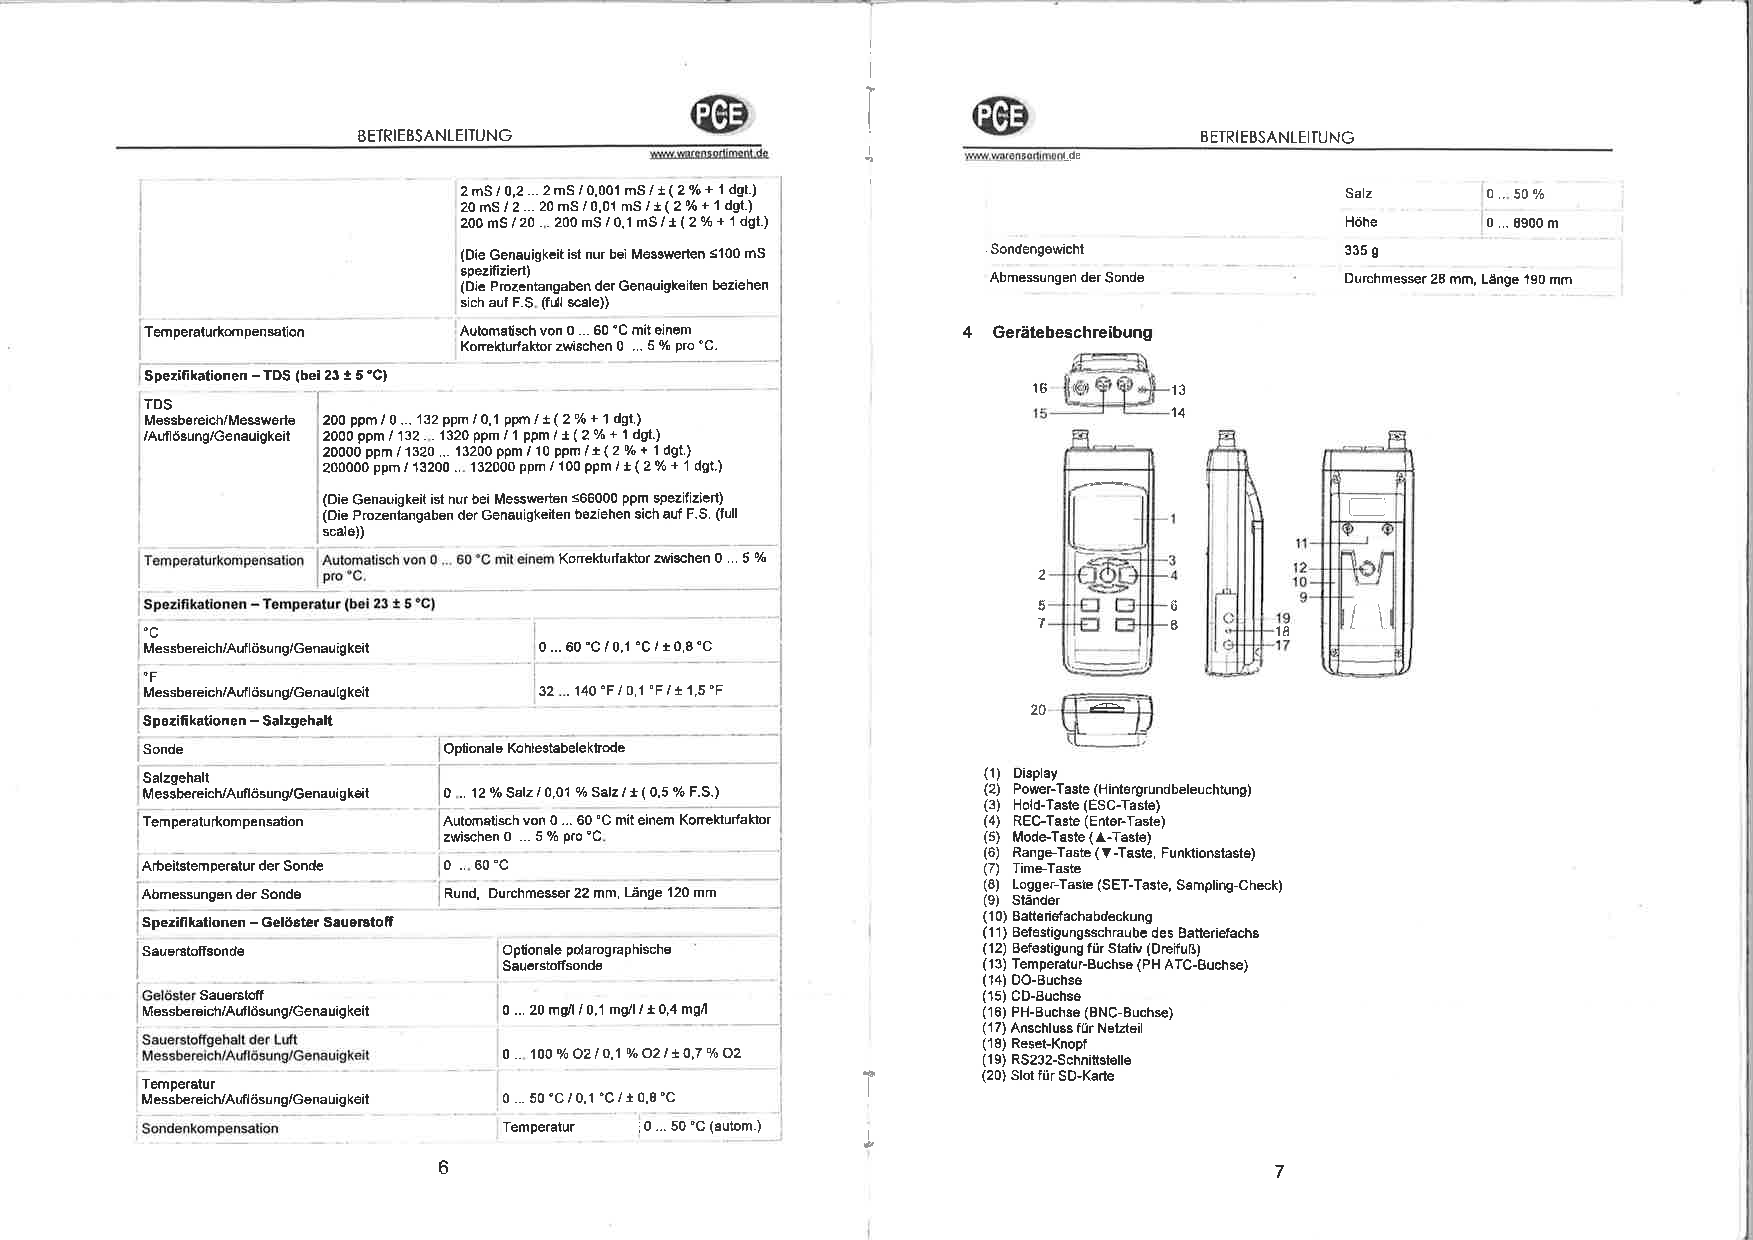
\includepdf[pages=1]{spez-sauerstofmesser2}

%\appendix
%\chapter*{Anhang}
%\addcontentsline{toc}{chapter}{Anhang}


\end{document}
